\RequirePackage{rotating}
\documentclass{article}

% Bibliography
\usepackage{natbib}
\bibpunct{(}{)}{;}{a}{}{;}

% Use 'It was found that A is B (Name 1234)' style
\setcitestyle{authoryear,open={},close={}}

% Affiliations
\usepackage{authblk}

\title{
  Quantifying the \new{impact} of an inference model 
  in Bayesian phylogenetics
}

\author[1,*]{Rich\`el J.C. Bilderbeek}
\author[1]{Giovanni Laudanno}
\author[1]{Rampal S. Etienne}
\affil[1]{Groningen Institute for Evolutionary Life Sciences, University of 
Groningen, Groningen, The Netherlands}
\affil[*]{corresponding author: r.j.c.bilderbeek@rug.nl}

% Use double spacing
\usepackage{setspace}
\doublespacing
\usepackage{listings}
\usepackage{hyperref}
\usepackage{todonotes}
\usepackage{verbatim}
\usepackage{pgf}
\usepackage{bm}
\usepackage{multirow}
\usepackage{amsfonts}
\usepackage{array}
\usepackage{array}
\usepackage{booktabs}
\newcolumntype{C}[1]{>{\centering\arraybackslash}p{#1}}
\newcolumntype{L}[1]{>{\raggedright\arraybackslash}p{#1}}
\usepackage{longtable}
\usepackage{rotating}
\usepackage{mathtools}
\usepackage{float}
\usepackage{tkz-graph}
\usetikzlibrary{arrows,automata}
\usetikzlibrary{calc}
\usetikzlibrary{arrows.meta}
\usepackage{rotating} % sidewaysfigure
\usepackage{doi}

% Style of listings
% From http://r.789695.n4.nabble.com/
%   How-to-nicely-display-R-code-with-the-LaTeX-package-listings-tp4648110.html
\usepackage{fancyvrb} 
\definecolor{codegreen}{rgb}{0,0.6,0}
\definecolor{codegray}{rgb}{0.5,0.5,0.5}
\definecolor{codepurple}{rgb}{0.58,0,0.82}
\definecolor{backcolor}{rgb}{0.95,0.95,0.92}
\lstdefinestyle{mystyle}{
  language=R,% set programming language
  basicstyle=\ttfamily\small,% basic font style
  commentstyle=\color{gray},% comment style
  % numbers=left,% display line numbers on the left side
  numberstyle=\scriptsize,% use small line numbers
  numbersep=10pt,% space between line numbers and code
  tabsize=2,% sizes of tabs
  showstringspaces=false,
  captionpos=b,% positioning of the caption below
  breaklines=true,% automatic line breaking
  escapeinside={(*}{*)},% escaping to LaTeX
  fancyvrb=true,% verbatim code is typset by listings
  extendedchars=false,% prohibit extended chars (chars of codes 128--255)
  alsoletter={.<-},% becomes a letter
  alsoother={$},% becomes other
  otherkeywords={!=, ~, $, \&, \%/\%, \%*\%, \%\%, <-, <<-, /},% other keywords
  deletekeywords={c}% remove keywords 
}
\lstset{style=mystyle}

% Adds numbered lines
\usepackage{lineno}
\linenumbers

% Rename 'Abstract' to 'Summary 
\usepackage[english]{babel}
\addto{\captionsenglish}{\renewcommand{\abstractname}{Summary}}

%comments
\newcommand{\giovanni}[1]{\textcolor{blue}{\textbf{[GL: #1]}}}
\newcommand{\richel}[1]{\textcolor{orange}{\textbf{[RB: #1]}}}
\newcommand{\rampal}[1]{\textcolor{green}{\textbf{[RSE: #1]}}}
\newcommand{\new}[1]{\textcolor{red}{#1}}
%\newcommand{\new}[1]{\textcolor{black}{#1}}

\begin{document}

\maketitle

\begin{abstract}

  \textbf{1. }
    Phylogenetic trees are currently routinely reconstructed from an alignment 
    of character sequences (usually nucleotide sequences). 
    Bayesian tools, such as MrBayes, RevBayes and BEAST2, 
    have gained much popularity over the last decade, 
    as they allow joint estimation of the posterior distribution of the 
    phylogenetic trees and the parameters of the underlying inference model.  
    An important ingredient of these Bayesian approaches is the species tree 
    prior.
    In principle, the Bayesian framework allows for comparing 
    different tree priors, which may elucidate the macroevolutionary 
    processes underlying the species tree.
    In practice, however, only macroevolutionary models that allow for fast computation of the prior probability are used.
    The question is how accurate the tree estimation is when the real macroevolutionary processes are substantially different from those assumed in the tree prior. \\
    \textbf{2. }
    Here we present \verb;pirouette;, 
    a free and open-source R package that assesses 
    the inference error made by Bayesian phylogenetics for a given macroevolutionary diversification model. \verb;pirouette; makes use of 
    BEAST2, but its philosophy applies to any Bayesian phylogenetic inference 
    tool. \\
  \textbf{3. }
    We describe \verb;pirouette;'s usage \new{providing full examples in which 
    we interrogate a model for its power to describe another}. \\
  \textbf{4. }
    Last, we discuss the results obtained by the examples and their 
    interpretation. \\
\end{abstract}

{\bf Keywords:} Bayesian model selection, BEAST2, computational biology, evolution, phylogenetics, R, tree prior

%%%%%%%%%%%%%%%%%%%%%%%%%%%%%%%%%%%%%%%%%%%%%%%%%%%%%%%%%%%%%%%%%%%%%%%%%%%%%%%%
\section{Introduction}
%%%%%%%%%%%%%%%%%%%%%%%%%%%%%%%%%%%%%%%%%%%%%%%%%%%%%%%%%%%%%%%%%%%%%%%%%%%%%%%%

The development of new powerful Bayesian phylogenetic inference tools, 
such as BEAST [\cite{drummond2007beast}], 
MrBayes [\cite{huelsenbeck2001mrbayes}]
or RevBayes [\cite{hohna2016revbayes}] 
has been a major advance in constructing phylogenetic trees 
from character data (usually nucleotide sequences) extracted
% 00004
from organisms (usually extant, but extinction events 
and/or time-stamped data can be added), 
and hence in our understanding of the main drivers 
and modes of diversification \richel{Reword this awkwardly long sentence}.


BEAST [\cite{drummond2007beast}] is a typical Bayesian phylogenetics tool, 
that needs both character data and priors to infer 
a posterior distribution of phylogenies.
Specifically, for the species tree prior - which describes 
the process of diversification - 
BEAST has built-in priors such as the Yule [\cite{yule}] and 
(constant-rate) birth-death [\cite{nee1994reconstructed}] models.
These simple tree priors are \new{among} the most commonly used, 
as they represent some biologically realistic processes (i.e. 
branching at per species constant rates), while being computationally fast.

\new{
  % 00002
  In this paper, we focus on BD models, instead of coalescent models,
  although these are just as important.
}

\new{
  % 00001
  To allow users to extend the functionalities of BEAST
  by using plug-ins, BEAST2 was written [\cite{bouckaert2019beast}]
  and both tools are still developed independently.
}

For example, one can add novel diversification models 
by writing a BEAST2 package that contains the likelihood 
formula of a phylogeny under the novel diversification model, 
i.e. the prior probability of a species tree.
Many diversification models (and their associated probability algorithms) 
have been developed, e.g., models in which diversification is time-dependent [\cite{nee1994reconstructed,rabosky2008explosive}],
or diversity-dependent [\cite{etienne2012diversity}],
or where diversification rates change for specific lineages 
and their descendants [\cite{etienne2012conceptual, rabosky2014automatic, alfaro2009nine}].
Other models treat speciation as a process that takes 
time [\cite{rosindell2010protracted, etienne2012prolonging, lambert2015reconstructed}],
or where diversification rate
depends on one or more traits [\cite{maddison2007estimating, fitzjohn2012diversitree}].
Despite such a rich theoretical landscape, only a few of these 
diversification models are available as tree priors in BEAST2
% 00005
\new{
  Despite the fact that some models are already included as tree priors 
  in BEAST2 (e.g. birth-death models, coalescent models, coalescent skyline, etc.) 
  many others for which a likelihood formula is already available 
  in literature, are not implemented yet.
}
% 00014
\new{
  BEAST2 allows to extend its functionality by plug-ins, such
  as the calibrated Yule model (\cite{heled2015calibrated}),
  BD with incomplete sampling (\cite{stadler2009incomplete}),
  BD serial sampling (\cite{stadler2012estimating}),
  BD serial skyline (\cite{stadler2013birth})
  Fossilized BD process (\cite{gavryushkina2014bayesian}),
  BD SIR (\cite{kuhnert2014simultaneous}) and many more.
}

When a novel diversification model is introduced,
its performance in inference should be tested.
Part of a model's performance is its ability to 
recover parameters from simulated data with known 
parameters (e.g. [\cite{etienne2014estimating}]), 
where ideally the estimated parameter values closely match the known/true values.
Even when a diversification model passes this procedure, 
it is not necessarily used as tree prior in Bayesian inference.
Bayesian phylogenetic inference often requires 
that the prior probability of the phylogeny 
according to the diversification model has to be computed millions of times. 
Therefore, biologically interesting but computationally expensive tree priors 
are often not implemented, and simpler priors are used instead. 
This is not necessarily problematic, when the data are very informative 
% 00010
\new{or when the prior is truly uninformative}, 
as this will reduce the influence of the tree prior.
However, the assumption that tree prior choice is of low \new{impact} 
must first be verified.

There have been multiple attempts to investigate the \new{impact} of tree
prior choice. For example, Sarver and colleagues, [\cite{sarver2019choice}] 
showed that the choice of tree prior does not 
substantially affect phylogenetic inferences of diversification rates.
However, they only compared current diversification models to one another, 
and thus this does not inform us on the \new{impact} of a new tree prior.

Here we introduce a method to quantify the \new{impact} of a novel tree prior.
The method starts with a phylogeny generated by the new model. 
Next, nucleotide sequences are simulated that follow the evolutionary 
history of the given phylogeny. 
Then, using BEAST2's built-in tree priors,
a Bayesian posterior distribution of phylogenies is inferred. 
We then compare the inferred with the original phylogenies. 
How to properly perform this comparison forms the heart of our method.
Only new diversification models that result 
in a large discrepancy between inferred and simulated phylogenies 
will be worth the effort and computational burden to implement 
a species tree prior for in a Bayesian framework.

Our method is programmed as an R package [\cite{R}] called \verb;pirouette;.
\verb;pirouette; is built on \verb;babette; [\cite{bilderbeek2018babette}], 
which calls BEAST2 [\cite{bouckaert2019beast}]. 

%%%%%%%%%%%%%%%%%%%%%%%%%%%%%%%%%%%%%%%%%%%%%%%%%%%%%%%%%%%%%%%%%%%%%%%%%%%%%%%%
\section{Description}
%%%%%%%%%%%%%%%%%%%%%%%%%%%%%%%%%%%%%%%%%%%%%%%%%%%%%%%%%%%%%%%%%%%%%%%%%%%%%%%%

The goal of \verb;pirouette; is to quantify the \new{impact} of a tree prior.
It does so by measuring the inference error made 
for a given reconstructed phylogeny, 
simulated under a (usually novel) diversification model.
We refer to the model that has generated the given tree
as the 'generative tree model' $\mathit{p_{G}}$.
\new{
  % 00006
  The error we aim to quantify is not of stochastic nature.
  Stochastic errors are usually non-directional.
  We, instead, aim to expose the bias due to the mismatch between generative and inference models.
}
We define the birth-death (BD) model [\cite{nee1994reconstructed}] as
the standard tree model, as many (non-standard) tree models 
have a parameter setting for which they reduce to this model. 
One such example is the diversity-dependent (DD) diversification 
model [\cite{DDD, etienne2012diversity}]:
the DD model is a \new{diversification model} with a speciation 
or extinction rate that depends 
on the number of species and a clade-level carrying capacity.
\new{ %00012
The BD model can be seen as a special case for the DD model. In fact, for} a carrying capacity
of infinity, the DD model reduces to the BD model.
When benchmarking a novel tree model, 
one will typically construct phylogenies 
for different combinations of the diversification model's parameters, 
to assess under which scenarios the inference error cannot be neglected. 
While we recommend many replicate simulations 
when assessing a novel tree prior, 
our examples contain only one replicate,
as the goal is to show the workings of \verb;pirouette;,
instead of doing an extensive analysis.
The supplementary material, however, does show the results
of replicated runs under multiple settings.

\verb;pirouette; allows the user to specify a wide variety of custom settings. 
These settings can be grouped in macro-sections, 
according to how they operate in the pipeline. 
We summarize them in Table~\ref{tab:options} and Table~\ref{tab:definitions}.

\begin{sidewaystable}
\centering
  \begin{tabular}{|p{3.4cm}|p{9.7cm}|p{4.5cm}@{}|}
    \hline
    \centering
    %%%%%%%%%%%%%%%%%%%%%%%%%%%%%%%%%%%%%%%%%%%%%%%%%%%%%%%%%%%%%%%%%%%%%%%%%%%%
    \textbf{Sub-argument} & 
    \textbf{Description} &
    \textbf{Possible values} \\ 
    \hline
    %%%%%%%%%%%%%%%%%%%%%%%%%%%%%%%%%%%%%%%%%%%%%%%%%%%%%%%%%%%%%%%%%%%%%%%%%%%%
    \verb;tree_prior; &
    Macroevolutionary diversification model &
    BD, CBS, CCP, CEP, Yule \\
    %%%%%%%%%%%%%%%%%%%%%%%%%%%%%%%%%%%%%%%%%%%%%%%%%%%%%%%%%%%%%%%%%%%%%%%%%%%%
    \verb;clock_model; &
    Clock for the DNA mutation rates &
    RLN, strict \\
    %%%%%%%%%%%%%%%%%%%%%%%%%%%%%%%%%%%%%%%%%%%%%%%%%%%%%%%%%%%%%%%%%%%%%%%%%%%%
    \verb;site_model; &
    Nucleotide substitution model &
    GTR, HKY, JC, TN \\
    %%%%%%%%%%%%%%%%%%%%%%%%%%%%%%%%%%%%%%%%%%%%%%%%%%%%%%%%%%%%%%%%%%%%%%%%%%%%
    \verb;mutation_rate; &
    Pace at which \new{substitutions occur} &
    \verb;mutation_rate; $\in \mathbb{R}_{>0}$\\
    %%%%%%%%%%%%%%%%%%%%%%%%%%%%%%%%%%%%%%%%%%%%%%%%%%%%%%%%%%%%%%%%%%%%%%%%%%%%
    \verb;root_sequence; &
    DNA sequence at the root of the tree &
    any combination of a, c, g, t \\
    %%%%%%%%%%%%%%%%%%%%%%%%%%%%%%%%%%%%%%%%%%%%%%%%%%%%%%%%%%%%%%%%%%%%%%%%%%%%
    \verb;model_type; &
    Criterion to select an inference model &
    Generative, Candidate \\
    %%%%%%%%%%%%%%%%%%%%%%%%%%%%%%%%%%%%%%%%%%%%%%%%%%%%%%%%%%%%%%%%%%%%%%%%%%%%
    \verb;run_if; &
    Condition under which an inference model is used &
    Always, Best candidate \\
    %%%%%%%%%%%%%%%%%%%%%%%%%%%%%%%%%%%%%%%%%%%%%%%%%%%%%%%%%%%%%%%%%%%%%%%%%%%%
    \verb;do_measure_evidence; &
    Sets whether or not the evidence of the model must be computed &
    TRUE, FALSE \\
    %%%%%%%%%%%%%%%%%%%%%%%%%%%%%%%%%%%%%%%%%%%%%%%%%%%%%%%%%%%%%%%%%%%%%%%%%%%%
    \verb;error_fun; &
    Specifies how to measure the error &
    nLTT, $|\gamma|$ \\
    %%%%%%%%%%%%%%%%%%%%%%%%%%%%%%%%%%%%%%%%%%%%%%%%%%%%%%%%%%%%%%%%%%%%%%%%%%%%
    \verb;burn_in_fraction; &
    Specifies the percentage of initial posterior trees to discard &
    \verb;burn_in_fraction; $\in [0, 1]$\\
    %%%%%%%%%%%%%%%%%%%%%%%%%%%%%%%%%%%%%%%%%%%%%%%%%%%%%%%%%%%%%%%%%%%%%%%%%%%%
    \hline
  \end{tabular}
  \caption{
    Most important parameter options.
    BD = birth death [\cite{nee1994reconstructed}], 
    CBS = coalescent Bayesian skyline [\cite{drummond2005bayesian}], 
    CCP = coalescent constant-population, 
    CEP = coalescent exponential-population,
    Yule = pure birth model [\cite{yule}],
    RLN = relaxed log-normal clock model [\cite{drummond2006relaxed}],
    strict = strict clock model [\cite{zuckerkandl1965molecules}], 
    GTR = Generalized time-reversible model [\cite{tavare1986some}], 
    HKY = Hasegawa, Kishino and Yano [\cite{hasegawa1985dating}], 
    JC = Jukes and Cantor [\cite{jukes1969evolution}], 
    TN = Tamura and Nei [\cite{tamura1993estimation}],
    nLTT = normalized lineages-through-time [\cite{janzen2015approximate}],
    $|\gamma|$ = absolute value of the gamma statistic [\cite{pybus2000testing}].
  }
  \label{tab:options}
\bigskip

  \begin{tabular}{|@{}c|p{4cm}|p{12.2cm}|}
    \hline
    \centering
    %%%%%%%%%%%%%%%%%%%%%%%%%%%%%%%%%%%%%%%%%%%%%%%%%%%%%%%%%%%%%%%%%%%%%%%%%%%%
    \textbf{Symbol} &
    \textbf{Macro-argument} &
    \textbf{Description} \\
    \hline
    %%%%%%%%%%%%%%%%%%%%%%%%%%%%%%%%%%%%%%%%%%%%%%%%%%%%%%%%%%%%%%%%%%%%%%%%%%%%
    $\mathit{G}$ &
    Generative model &
    The full setting to produce BEAST2 input data. 
    Its core features are the tree prior $\mathit{p_{G}}$, the clock 
    model $\mathit{c_{G}}$ and the site model $\mathit{s_{G}}$. \\
    %%%%%%%%%%%%%%%%%%%%%%%%%%%%%%%%%%%%%%%%%%%%%%%%%%%%%%%%%%%%%%%%%%%%%%%%%%%%  
    $\mathit{A}$ &
    Alignment model &
    Specifies the alignment generation, such as the clock model 
    $\mathit{c_{G}}$, site model $\mathit{s_{G}}$ and root sequence. \\
    %%%%%%%%%%%%%%%%%%%%%%%%%%%%%%%%%%%%%%%%%%%%%%%%%%%%%%%%%%%%%%%%%%%%%%%%%%%%
    $\mathit{X_{i}}$ &
    $i$-th candidate experiment &
    Full setting for a Bayesian inference. It is made by a 
    candidate inference model $\mathit{I_{i}}$ and its 
    inference conditions $\mathit{C_{i}}$. \\
    %%%%%%%%%%%%%%%%%%%%%%%%%%%%%%%%%%%%%%%%%%%%%%%%%%%%%%%%%%%%%%%%%%%%%%%%%%%%
    $\mathit{I}$ &
    Inference model &
    The assumed phylogenetic inference model, of which the main components
    are the tree prior $\mathit{p_{I}}$, assumed clock model $\mathit{c_{I}}$ 
    and assumed site model $\mathit{s_{I}}$. \\
    %%%%%%%%%%%%%%%%%%%%%%%%%%%%%%%%%%%%%%%%%%%%%%%%%%%%%%%%%%%%%%%%%%%%%%%%%%%%
    $\mathit{C}$ & Inference conditions & Conditions under which $\mathit{I}$ 
    is used in the inference. 
    They are composed of the model type, run condition and 
    whether to measure the evidence. \\
    %%%%%%%%%%%%%%%%%%%%%%%%%%%%%%%%%%%%%%%%%%%%%%%%%%%%%%%%%%%%%%%%%%%%%%%%%%%%
    $\mathit{E}$ & Error measure parameters & 
    Errors measurement setup that can be specified providing an 
    error function to measure the difference between the original phylogeny 
    and the inferred posterior. The first iterations of the MCMC chain of the 
    posterior may not be representative and can be discarded using a burn-in 
    fraction. \\
    %%%%%%%%%%%%%%%%%%%%%%%%%%%%%%%%%%%%%%%%%%%%%%%%%%%%%%%%%%%%%%%%%%%%%%%%%%%%
    \hline 
  \end{tabular}
  \caption{
    Definitions of terms and relative symbols used in the main text and in 
    Fig~\ref{fig:pipeline}. To run the pipeline $\mathit{A}$, $\mathit{X}$ 
    and $\mathit{E}$ must be specified.
  }
  \label{tab:definitions}
\end{sidewaystable}

\subsection{pirouette's pipeline}
\label{subsec:pipeline}

\begin{figure}
  \centering
  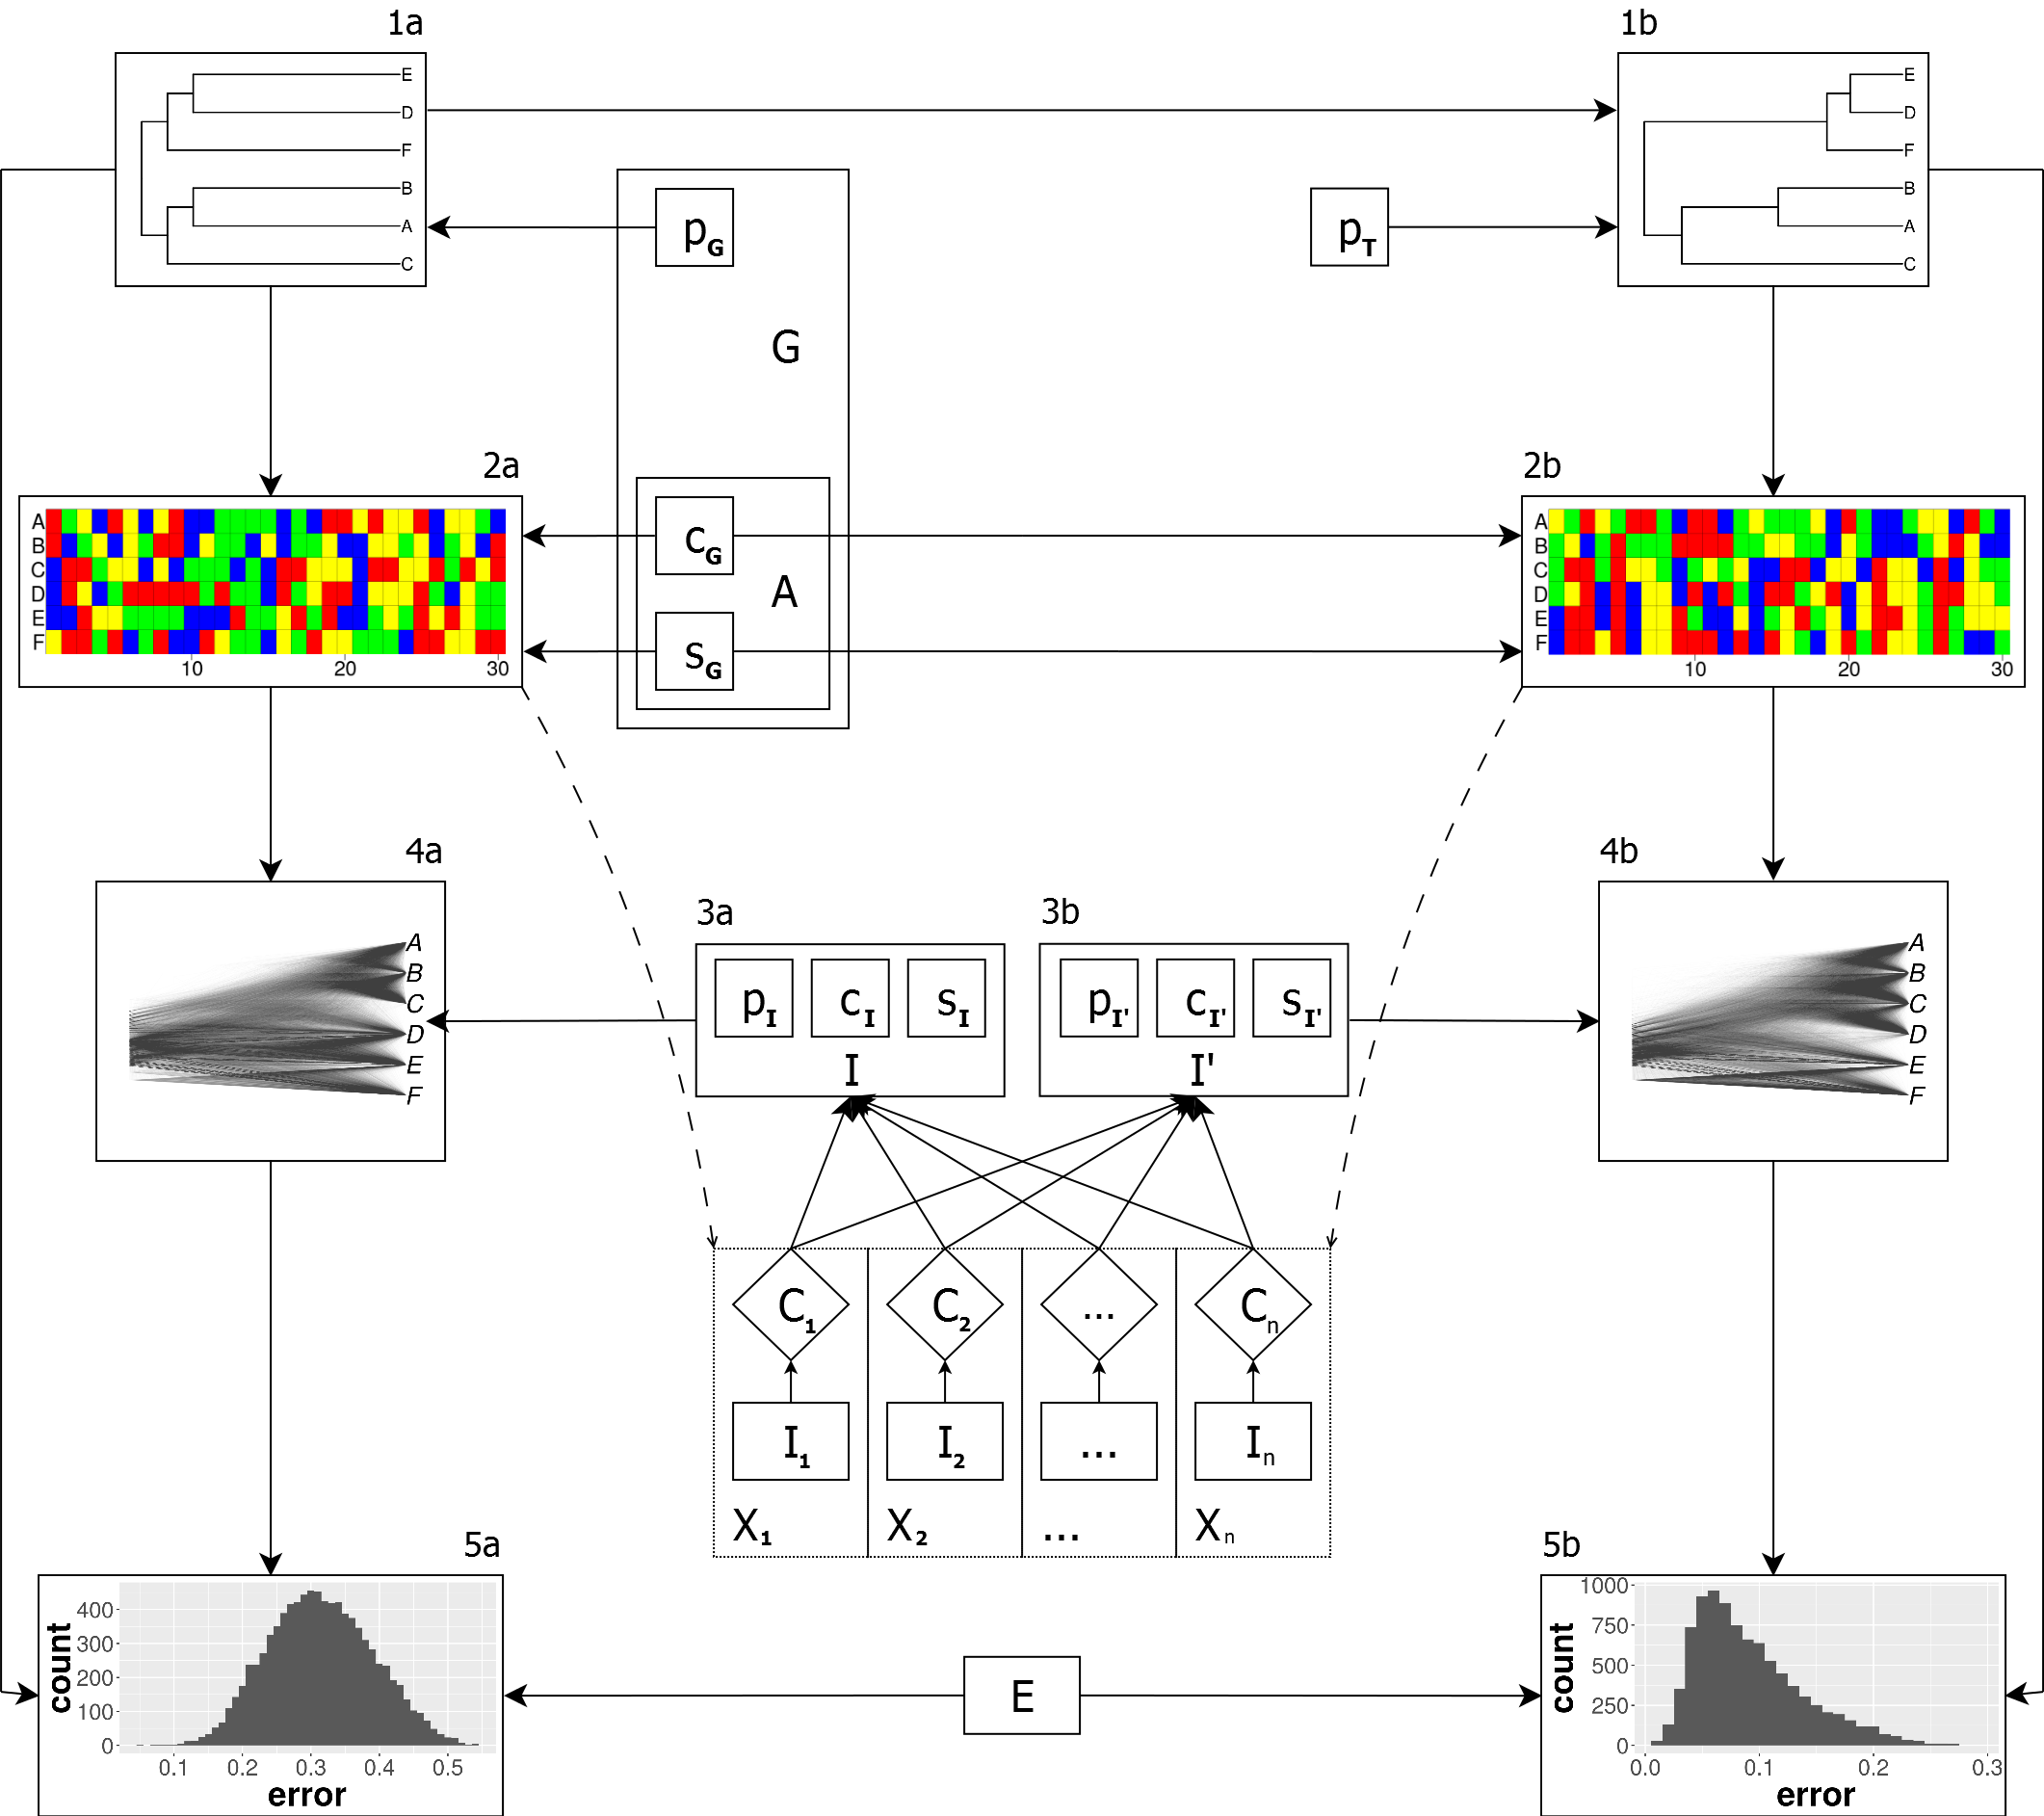
\includegraphics[width = 0.99\textwidth]{workflow4.png}
  \caption{
    \texttt{pirouette} pipeline.
    The pipeline starts from a phylogeny (1a) simulated by the 
    generative tree model 
    $\mathit{p_{G}}$.
    The phylogeny is converted to an alignment (2a) using the generative 
    alignment model 
    $\mathit{A} = (\mathit{c_{G}}, \mathit{s_{G}})$, composed of a clock model and a site model. 
    The user defines one or more experiments.
    For each candidate experiment $\mathit{X_{i}}$ 
    (a combination of inference model $\mathit{I_{i}}$ and condition $\mathit{C_{i}}$),
    if its condition $\mathit{C_{i}}$ is 
    satisfied (which can depend on the alignment), 
    the corresponding inference model $\mathit{I} = \mathit{I_{i}}$ is selected
    to be used in the next step.
    The inference models (3a) of the selected experiments use the alignment (2a) 
    to each create a Bayesian posterior of (parameter estimates and) 
    phylogenies (4a). 
    Each of the posteriors' trees is compared to the true phylogeny (1a) 
    using the error measure $\mathit{E}$, 
    resulting in an error distribution (5a). 
    Optionally, for each selected inference model a twin pipeline can be run.
    A twin phylogeny (1b) can be generated from the original 
    phylogeny (1a) using the twin tree model $\mathit{p_{t}}$, 
    selected among standard diversification models; 
    the default option is the standard BD model, 
    with parameters estimated from the original phylogeny.
    A twin alignment (2b) is then simulated from the twin phylogeny 
    using clock model $\mathit{c_{G}}$ and site model $\mathit{s_{G}}$ 
    imported from the generative model. 
    The twin pipeline follows the procedure of the main pipeline, 
    resulting in a twin error distribution (5b).
  }
  \label{fig:pipeline}
\end{figure}

The pipeline to assess the error BEAST2 makes in inferring this phylogeny 
contains the following steps:
\begin{enumerate}
  \item The user supplies one or (ideally) more phylogenies from a 
    new diversification model.
  \item From the given phylogeny an alignment is simulated 
    under a known alignment model $\mathit{A}$.
  \item From this alignment, according to the specified 
    inference conditions $\mathit{C}$, 
    an inference model $\mathit{I}$ is chosen (which may differ from the 
    generative model).
  \item The inference model and the alignment are used 
    to infer a posterior distribution of phylogenies.
  \item The phylogenies in the posterior are compared with the given phylogeny 
    to estimate the error made, according to 
    the error measure $\mathit{E}$ specified by the user.
\end{enumerate}

The pipeline is visualized in Fig.~\ref{fig:pipeline}. 
There is also the option to generate a 'twin tree', 
that goes through the same pipeline. 
The utility of this twin tree will be explained below.

The first step simulates an alignment from the given 
phylogeny (Fig.~\ref{fig:pipeline}, 1a $\rightarrow$ 2a).
For the sake of clarity, here we will assume the alignment consists
of DNA sequences, but one can also use other heritable material such as amino acids.
The user must specify a root sequence, a mutation rate and a site model.
\iffalse
The root sequence is the DNA sequence of the shared common ancestor of 
all species, and is set to four different equally-sized 
mononucleotide blocks by default, 
which helps interpreting the resulting alignment.
\fi
\new{ % 00008
The root sequence is the DNA sequence of the shared common ancestor of 
all species. By default it is set to four different equally-sized 
mononucleotide blocks (a block of length $n$ is a sequence in which the same character is repeated $n$ times), which helps interpreting the resulting alignment.
}
Supported nucleotide substitution models (part of a DNA
site model) are JC, HKY, TN and GTR (see Table \ref{tab:options} for
the meaning of these abbreviations).
JC is the default nucleotide substitution model (NSM),
in which the nucleotide substitution rates between all
nucleotides are equal and constant over time.

The second step (Fig.~\ref{fig:pipeline}, 3a)
selects one or more inference model(s) $I$ from 
a set of standard inference models $I_{1},\dots,I_{n}$.
For example, if the generative model is known and standard,
one can specify the inference model to be the same as the generative model.
If the tree model is unknown or non-standard - which is the primary motivation for this paper -, one can pick
a standard inference model which is considered to be closest to the true tree model.
Also, if we want to run only the inference
model that fits best to an alignment from a set of candidates,
one can specify these inference models as 
well (see section 'Candidate models').

The third step infers the posterior distributions,
using the simulated alignment (Fig.~\ref{fig:pipeline}, 2a $\rightarrow$ 4a),
and the inference models that were selected in the previous step (3a). 
For each selected experiment a posterior distribution is inferred, using the 
\verb;babette; [\cite{bilderbeek2018babette}] R package which makes use of BEAST2. 
This step usually takes up most of the pipeline's computation time.

The fourth step quantifies the inference error made. 
First the burn-in fraction is removed, i.e. the first phase of the 
Markov chain Monte Carlo (MCMC) run,
which samples an unrepresentative part of parameter and tree space. 
By default, \verb;pirouette; 
removes the first 10\% of the posterior.
From the remaining posterior, \verb;pirouette; 
creates an error distribution, by measuring the difference
between the true tree and each of the posterior 
trees (Fig.~\ref{fig:pipeline}, 4a $\rightarrow$ 5a).
The user can specify a function to quantify the differences between
the true and posterior trees. By default, the package uses the nLTT 
statistic [\cite{janzen2015approximate}], which is the absolute difference
between the normalized lineages-through-time plots of two trees.
The nLTT statistic is chosen, as it can operate on any two trees (regardless
of their crown ages and number of taxa) and its results have a clear range
from zero to one. This normalized result makes it possible to compare trees 
from a distribution of trees from any tree model.

\subsection{Twinning}\label{subsec:twinning}

Similar to lab experiments, \verb;pirouette; allows to perform
a control measurement, by use of a process we call twinning. 
In this context, this control results in an error distribution
that is the baseline error of the pipeline. The difference
between the 'true' and 'twin' error distributions is caused only
by the mismatch between the generative tree model and the assumed
tree prior.

The twinning process, $T$, encompasses two steps:
$T_1$, that generates a 'twin tree' (Fig.~\ref{fig:pipeline}, 1b) 
and $T_2$, which generates a 'twin alignment' (Fig.~\ref{fig:pipeline}, 2b).
Both twin tree and alignment will be analyzed in the same way 
as the true tree and alignment.

We define a phylogeny $\tau$ as the combination of
branching times $\Vec{t}$ and topology $\psi$, 
and denote as $\tau_{\mathit{G}}$ the phylogeny 
produced by a (possibly non-standard) generative diversification model, 
having branching times $\Vec{t}_{\mathit{G}}$ and 
topology $\psi_{\mathit{G}}$.

The first step ($T_1$) of the twinning process creates a tree $\tau_{\mathit{T}}$
with branching times $\Vec{t}_{\mathit{T}}$ while preserving the original
topology $\psi_{\mathit{G}}$:
\begin{align}
  \tau_{\mathit{G}} = (\Vec{t}_{\mathit{G}}, \psi_{\mathit{G}}) 
  \xrightarrow[]{\mathit{T_1}} 
  \tau_{\mathit{T}} = (\Vec{t}_{\mathit{T}}, \psi_{\mathit{G}})
\end{align}

\new{
  % 00007
  We choose to preserve the original topology to 
  increase the similarity between the twin to the original tree. 
  This works well in the cases of the birth-death or diversity-dependent models 
  we consider in our examples.
  However, this might not be suited for models in which branching times 
  are strongly influenced by topology.
}

\new{
  % 00003
  The default option for the twin diversification model $p_T$ 
  is to use the standard BD model.
}
\new{
  % 00009
  pirouette has a built-in function to use a Yule model as well.
  Additionally, a user can specify a function to generate a twin tree
  from any speciation model, such as, for example, a coalescent model.
}

It is then possible to use the likelihood function 
$L_{\mathit{T}}$ for this diversification model to find 
the parameters $\theta^{*}_{\mathit{T}}$ 
(e.g. speciation and extinction rates, in case of a BD model) 
that maximize this likelihood applied 
to the true tree, conditioned on its number of tips $n_{\mathit{G}}$:
\begin{align}
    \max[L_{\mathit{T}}(\theta_{\mathit{T}}|\tau_{\mathit{G}}, n_{\mathit{G}})] 
\rightarrow \theta^{*}_{\mathit{T}}.
\end{align}
We use $\theta^{*}_{\mathit{T}}$ to simulate a number 
$n_{\mathit{T}} = n_{\mathit{G}}$ 
of branching times $\Vec{t}_{\mathit{T}}$ for the twin tree 
$\tau_{\mathit{T}}$, under the process $p_{T}$, 
while preserving the topology. 
We simulate the new branching times using the TESS 
package [\cite{TESS, hohna2016tess}].
\new{ %00013
For simplicity, when simulating phylogenies we assumed a sampling fraction of $100\%$. A different choice might have an effect on model performance.
}

The second step ($T_2$) of the twinning process simulates the twin alignment 
with the same clock model, site model and mutation rate 
used to simulate the original alignment. 
The twin alignment can be simulated in any user-defined way.
\verb;pirouette; supplies the option to have it simulated with
the same mutation rate as the true alignment. By default, however,
not only the same mutation rate is used, but also the total number of \new{substitution}s
matches the true alignment. The total number of \new{substitution}s is defined
as the amount of different nucleotides between the (known) root sequence
compared to the sequences at the tips.

\subsection{Candidate models}\label{subsec:candidates}

The user has to specify exactly one standard inference model,
but may be unsure which one to pick. To account for this, the user can
specify a set of candidate inference models. Each of these candidate inference models is run in an initial, relatively short, analysis; the candidate model with the highest 
evidence (i.e., marginal likelihood) will then be
used in another, longer, inference run, resulting in another error distribution.
The evidence for an inference model is estimated by nested 
sampling [\cite{russel2019model}], using the \verb;NS; BEAST2 package. 

If twinning is used, a candidate model that has the highest evidence for
the twin alignment is also used to create another error
distribution.

\subsection{Stochasticity caused by simulating phylogenies}

Finally, if the goal is to evaluate BEAST2's performance 
on a non-standard tree model, 
one must also consider the last source of stochasticity: 
the different phylogenies a tree model generates.
A single phylogeny cannot be considered as fully representative of the model. 
For this reason multiple phylogenies must be considered. 
If the number of considered phylogenies is high enough, 
the comparison between the main pipeline's aggregated error distribution 
and its twin counterpart leads to a fair evaluation 
of the new tree model with respect to the baseline error.

%%%%%%%%%%%%%%%%%%%%%%%%%%%%%%%%%%%%%%%%%%%%%%%%%%%%%%%%%%%%%%%%%%%%%%%%%%%%%%%%
\section{Usage}
%%%%%%%%%%%%%%%%%%%%%%%%%%%%%%%%%%%%%%%%%%%%%%%%%%%%%%%%%%%%%%%%%%%%%%%%%%%%%%%%

We show the usage of \verb;pirouette; on a tree generated 
by the non-standard diversity-dependent (DD) tree 
model [\citep{DDD, etienne2012diversity}],
which is a BD model with a speciation rate that is dependent on the number of species. 
\new{ %00011
The example we propose here has only an instructional purpose. To perform a full analysis we suggest to repeat the same procedure for at least 100 independent true and twin trees (we show the outcome of an analysis involving replicates in the supplementary material at subsection \ref{subsec:distribution}).
}

The code to reproduce our results can be found at  
\url{https://github.com/richelbilderbeek/pirouette_example_30}
and a simplified version is shown here for convenience:

\begin{lstlisting}[language=R]
library(ggplot2)
library(pirouette)

# Create phylogeny
phylogeny <- create_exemplary_dd_tree(
  n_taxa = 6, 
  crown_age = 10,
  extinction_rate = 0.1
)

# Use standard pirouette setup
pir_params <- create_std_pir_params()

# Do the runs
pir_out <- pir_run(
  phylogeny = phylogeny,
  pir_params = pir_params
)

# Plot
pir_plot(pir_out)

# Save
pir_save(
  phylogeny = phylogeny,
  pir_params = pir_params,
  pir_out = pir_out,
  folder_name = "example_30"
)
\end{lstlisting}

The DD tree that is generated by this code is as shown in Figure \ref{fig:dd_tree},
which has an arbitrarily chosen crown age of 10 time units and 6 tips 
for an extinction rate of 0.1. The carrying-capacity is also set at 6. The initial speciation rate $\lambda_0$ is chosen such that the expected number of species in a constant-rate BD model would be equal to the number of tips, which amounts to $\lambda_0 = 0.63$.

\begin{figure}[H]
  \includegraphics[width=\textwidth]{pirouette_example_30/example_30_314/true_tree.png}
  \caption{
    The example tree resulting from a diversity-dependent (DD) simulation.
  }
  \label{fig:dd_tree}
\end{figure}

Using the default \verb;pirouette; settings,
the error distribution shown in Figure \ref{fig:example_30}
is produced.

\begin{figure}[H]
  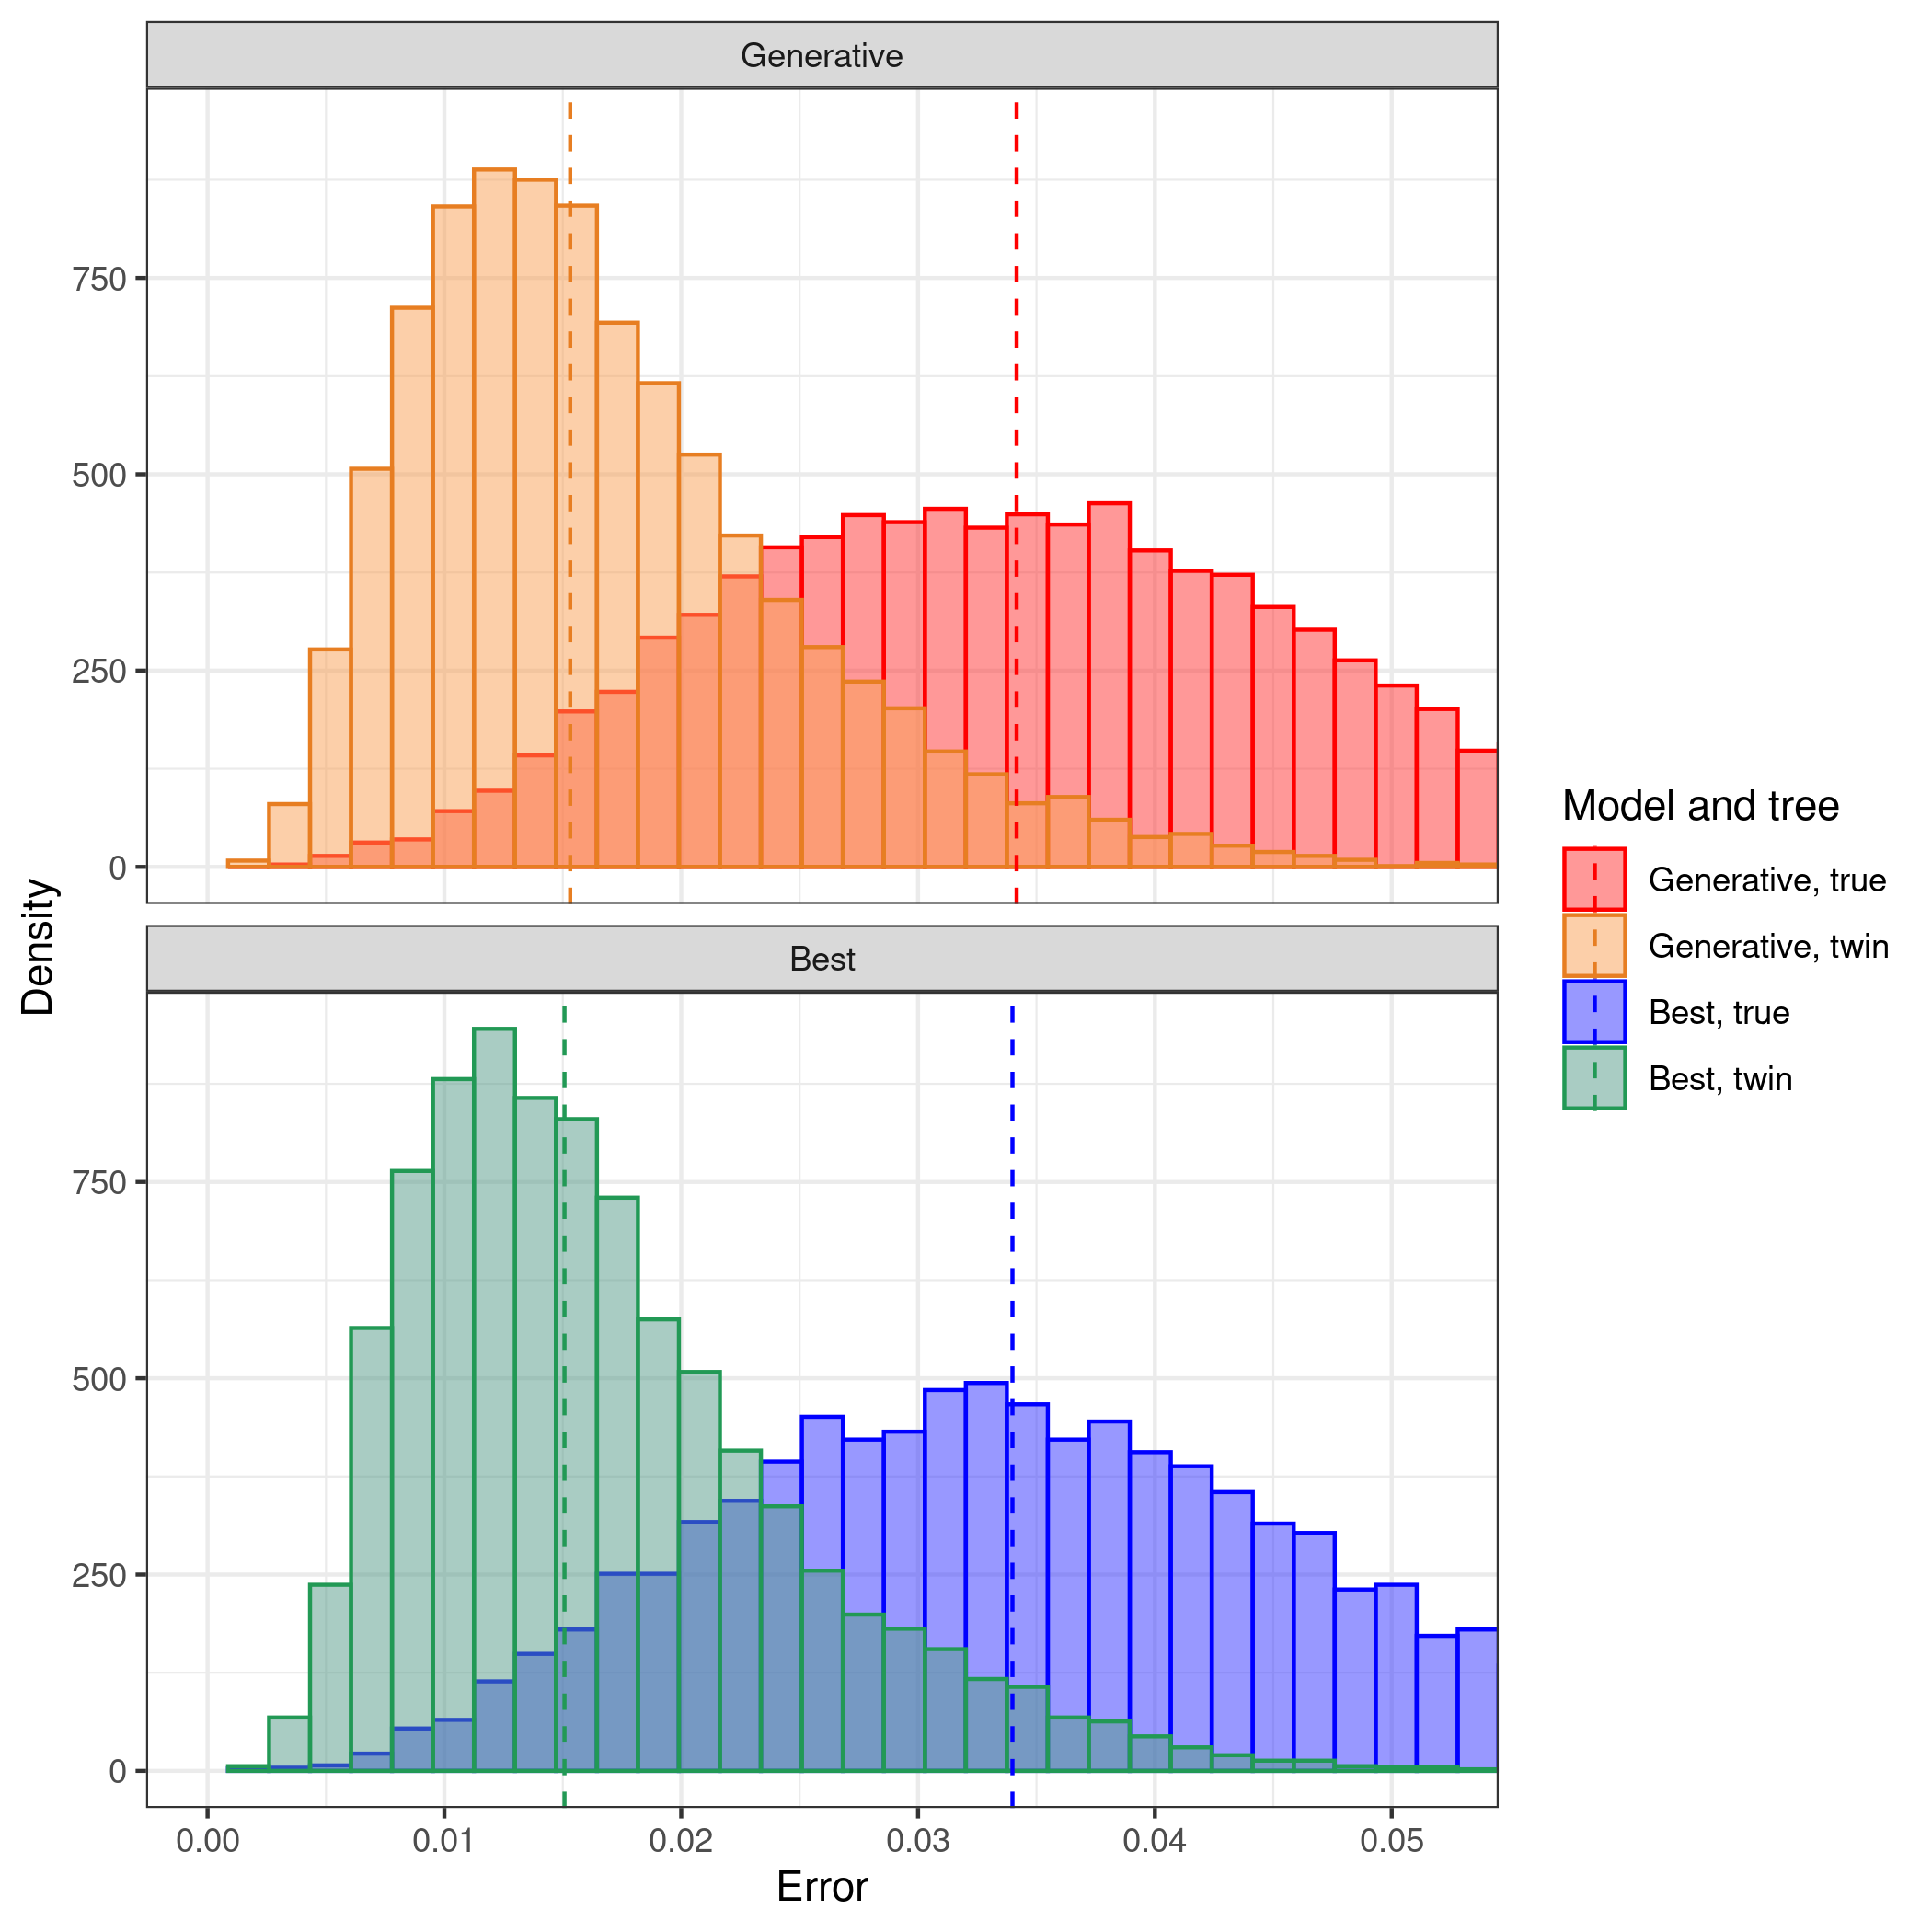
\includegraphics[width=\textwidth]{pirouette_example_30/errors.png}
  \caption{
    The inference error made 
    for an assumed generative tree model and best candidate model,
    compared with the error obtained for the twin tree.
    The assumed generative tree model is the model assumed to be closest to
    the actual generative tree model that generated the true tree.
    The twin distributions show the baseline inference error.
    Vertical dashed lines show the median error value per distribution.
  }
  \label{fig:example_30}
\end{figure}

In the upper panel of Figure \ref{fig:example_30},
we can see that the error distributions of the assumed generative model
differ strongly between the true and twin tree. 
This difference shows the extent of the mismatch between
the actual tree model (which is DD) and the (BD) tree prior used.
Because these distributions are distinctively different,
the inference error we make when using an 
incorrect (that is, BD) tree prior on a DD tree
is profound.

Comparing the upper and lower panel of Figure \ref{fig:example_30}, 
we can see that the best
candidate model is only slightly better at inferring the true tree,
than the assumed generative model, thereby showing that they cannot compensate for the true generative tree model not being among the inference models.

The candidate model that had highest evidence given the simulated alignment,
was JC, RLN, BD (see Table \ref{tab:options} for the meaning of these 
abbreviations). JC was indeed the site model used when simulating the
alignments. The RLN clock model is an unexpected choice: the RLN clock
model assumes that mutation rates differ between lineages, whereas the
alignment was simulated with equal mutation rates for all lineages.
The BD model is indeed closer to the DD model than Yule, as both BD and DD
model allow for extinction, while Yule does not.

%%%%%%%%%%%%%%%%%%%%%%%%%%%%%%%%%%%%%%%%%%%%%%%%%%%%%%%%%%%%%%%%%%%%%%%%%%%%%%%%
\section{Discussion}
%%%%%%%%%%%%%%%%%%%%%%%%%%%%%%%%%%%%%%%%%%%%%%%%%%%%%%%%%%%%%%%%%%%%%%%%%%%%%%%%

We showed how to use \verb;pirouette; to quantify the \new{impact} of a 
tree prior in Bayesian phylogenetics, assuming the simplest standard 
tree model possible.
In principle any other standard tree model can be assumed, 
but we chose to provide the simplest example.

Figure~\ref{fig:example_30} illustrates the primary result of our pipeline: 
it shows the error distributions for the true tree and the twin tree 
when either the (assumed) generating model or the best candidate model is used in inference. 
The clear difference between the error distributions 
for the true tree and the twin tree suggests 
that the choice of tree prior does matter.
We note, however, that only one tree from a novel tree model
is not enough to determine the \new{impact} of using an incorrect
tree prior. Instead, a distribution 
of multiple trees, generated by the novel tree model, should be used. In the supplementary material we have provided some examples.

Like most phylogenetic experiments, the setup of \verb;pirouette;
involves many choices. A prime example is the
length of the simulated DNA sequence. One expects that the inference error
decreases for longer DNA sequences. We investigated this
superficially and confirmed this prediction (see the supplementary materials). 
However, we note that for longer DNA sequences, the assumption 
of constant substitution rates may become less realistic 
and hence longer sequences may require more parameters. 
Hence, simply getting longer sequences will not always lead to a drastic 
reduction of the influence of the species tree prior.
Fortunately, \verb;pirouette; provides a pipeline that works for all choices.

Interpreting the results of \verb;pirouette; is up to the user; 
\verb;pirouette; does not answer the question 
whether the inference error is too large to trust the inferred tree. The user is encouraged to use different statistics to measure the error. The nLTT statistic is
a promising starting point, as it can compare any two trees and 
results in an error distribution of known range, but one may also explore other statistics.
In principle, \verb;pirouette; allows for this, but in our example we used a diversification model (DD) that only deviates from the Yule and BD models in the temporal branching pattern, not in the topology.
\new{
    % 00007
    For models that make different predictions on topology, the twinning process should be modified in line with it.
}

As noted in the introduction, Duch\^{e}ne and colleagues [\cite{duchene2018phylodynamic}],
also developed a method to assess the adequacy of a tree model
on empirical trees. They simulate trees from the posterior distribution of the parameters and then compare this to the originally inferred tree using tree statistics, to determine whether the assumed tree model in inference indeed generates the tree as inferred. This is useful if these trees match, but when they do not, this does not mean that the inferred tree is incorrect; if sufficient data is available the species tree prior may not be important, and hence the inference may be adequate even though the assumed species tree prior is not. In short, the approach is applied to empirical trees and compares the posterior and prior distribution of trees (with the latter generated with the posterior parameters!).
\verb;pirouette; aims to identify when assuming standard priors for the species tree leads to incorrect inference if one believes more complex diversification models are operating than can be currently accommodated in inference. In short, our approach applies to simulated trees and compares the posterior distributions of trees generated with a standard and non-standard model, but inferred with a standard one. The two methods therefore complement one another.

However, we note that the \verb;pirouette; pipeline is not restricted 
to exploring the effects of a new species tree model. 
The pipeline can also be used to explore the effects of non-standard 
clock or site models, such as relaxed clock models with a non-standard 
distribution, correlated substitutions on sister lineages, or elevated 
substitutions rates during speciation events. 
It is, however, beyond the scope of this paper to discuss all these options 
in more detail.

In conclusion, \verb;pirouette; can show the errors to be expected
when the model assumed in inference is different from the 
actual generative model.
The user can then judge whether or not this new model should be implemented in our Bayesian phylogenetic tool. 

%%%%%%%%%%%%%%%%%%%%%%%%%%%%%%%%%%%%%%%%%%%%%%%%%%%%%%%%%%%%%%%%%%%%%%%%%%%%%%%%
\section{Acknowledgments}
%%%%%%%%%%%%%%%%%%%%%%%%%%%%%%%%%%%%%%%%%%%%%%%%%%%%%%%%%%%%%%%%%%%%%%%%%%%%%%%%

We thank the Center for Information Technology of the University 
of Groningen for its support and for providing access to the Peregrine 
high performance computing cluster. 
We thank the Netherlands 
Organization for Scientific Research (NWO) for financial support 
through a VICI grant awarded to RSE.

%%%%%%%%%%%%%%%%%%%%%%%%%%%%%%%%%%%%%%%%%%%%%%%%%%%%%%%%%%%%%%%%%%%%%%%%%%%%%%%%
\section{Data Accessibility}
%%%%%%%%%%%%%%%%%%%%%%%%%%%%%%%%%%%%%%%%%%%%%%%%%%%%%%%%%%%%%%%%%%%%%%%%%%%%%%%%

All code is archived at 
\url{http://github.com/richelbilderbeek/pirouette_article},
with DOI \url{https://doi.org/12.3456/zenodo.1234567}.

%%%%%%%%%%%%%%%%%%%%%%%%%%%%%%%%%%%%%%%%%%%%%%%%%%%%%%%%%%%%%%%%%%%%%%%%%%%%%%%%
\section{Author contributions}
%%%%%%%%%%%%%%%%%%%%%%%%%%%%%%%%%%%%%%%%%%%%%%%%%%%%%%%%%%%%%%%%%%%%%%%%%%%%%%%%

RJCB, GL and RSE conceived the idea for the package. 
RJCB created, tested and revised the package.
GL provided major contributions to the package.
RJCB wrote the first draft of the manuscript, 
GL and RSE contributed to revisions.

%%%%%%%%%%%%%%%%%%%%%%%%%%%%%%%%%%%%%%%%%%%%%%%%%%%%%%%%%%%%%%%%%%%%%%%%%%%%%%%%
% Bibliography
%%%%%%%%%%%%%%%%%%%%%%%%%%%%%%%%%%%%%%%%%%%%%%%%%%%%%%%%%%%%%%%%%%%%%%%%%%%%%%%%
% MEE style
\bibliographystyle{pirouette_mee}
\bibliography{pirouette_article}
%%%%%%%%%%%%%%%%%%%%%%%%%%%%%%%%%%%%%%%%%%%%%%%%%%%%%%%%%%%%%%%%%%%%%%%%%%%%%%%%



%%%%%%%%%%%%%%%%%%%%%%%%%%%%%%%%%%%%%%%%%%%%%%%%%%%%%%%%%%%%%%%%%%%%%%%%%%%%%%%%
\section{Supplementary material}
%%%%%%%%%%%%%%%%%%%%%%%%%%%%%%%%%%%%%%%%%%%%%%%%%%%%%%%%%%%%%%%%%%%%%%%%%%%%%%%%

This supplementary material contains additional facets of \verb;pirouette;, 
such as the installation of the package, an overview of
pirouette's main functions and a guide for users, based on multiple experiments
that are shown here as well.

For these experiments, we limited the number of replicates by time, 
aiming at a duration of
24 hours per setting, when run on the Peregrine computer cluster of the
University of Groningen. Due to this, for example, a run of 40 taxa only
has 6 replicates, because one run takes 4 hours. For all experiments, the intermediate results can all be downloaded 
from their respective websites, which is approximately 5 gigabyte in total.

All the figures shown in this section are shown without any aesthetical modifications, with the exception that the arrangement
of the sub-figures in subsection \ref{subsec:main_example},
where we aligned parts of the figure by hand.

Here is an overview of the various sections:

\begin{itemize}
  \item{
    subsection \ref{subsec:guidelines}: guidelines for users
  }
  \item{
    subsection \ref{subsec:installation}: installation
  }
  \item{
    subsection \ref{subsec:resources}: resources, such as 
    website, tutorials, packages used, bug reporting and contributing
  }
  \item{
    subsection \ref{subsec:citation}: citation of pirouette
  }
  \item{
    subsection \ref{subsec:twinning}: the
    twinning process
  }
  \item{
    subsection \ref{subsec:candidates}: candidate models for the inference
  }
  \item{
    subsection \ref{subsec:stochasticity}: the effects of stochasticity
  }
  \item{
    subsection \ref{subsec:nltt}: the
    nLTT statistic
  }
  \item{
    subsection \ref{subsec:main_functions}: main functions
  }
  \item{
    subsection \ref{subsec:main_example}: code, extra figures and
    diagnostics regarding the main example.
  }
  \item{
    subsection \ref{subsec:distribution}: the result of using 
    multiple trees, as generated by the
    same stochastic process as the main example
  }
  \item{
    subsection \ref{subsec:n_taxa}: the effect of the number of taxa
  }
  \item{
    subsection \ref{subsec:n_nucleotides}: the effect of the DNA
    alignment sequence length
  }
  \item{
    subsection \ref{subsec:simplest_correct_parameterization} shows the
    effect when performing inference in the simplest use case
  }
  \item{
    subsection \ref{subsec:under_parameterization} shows the
    effect when performing inference with an under-parameterization
  }
  \item{
    subsection \ref{subsec:different_n_mutations} shows the
    effect when the twin alignment is allowed to have a different
    number of \new{substitution}s
  }
  \item{
    subsection \ref{subsec:mutation_rate} shows the
    effect of different mutation rates
  }
  \item{
    subsection \ref{subsec:acknowledgments}: Acknowledgments
  }
  \item{
    subsection \ref{subsec:data_accessibility}: Data accessibility
  }
  \item{
    subsection \ref{subsec:author_contributions}: Author contributions
  }
\end{itemize}


%%%%%%%%%%%%%%%%%%%%%%%%%%%%%%%%%%%%%%%%%%%%%%%%%%%%%%%%%%%%%%%%%%%%%%%%%%%%%%%%
\subsection{Guidelines for users}
\label{subsec:guidelines}
%%%%%%%%%%%%%%%%%%%%%%%%%%%%%%%%%%%%%%%%%%%%%%%%%%%%%%%%%%%%%%%%%%%%%%%%%%%%%%%%

From the experiments shown below, we composed some rough guidelines.
These guidelines should be treated as preliminary results, as
the total runtime of these experiments is 'only' 19 days.

\begin{itemize}
  \item{
    The use of 20 replicates results in decent plots.
  }
  \item{
    The use of more taxa increases the inference error
  }
  \item{
    The use of longer DNA sequences decreases the inference error.
  }
  \item{
    When we do not impose the same number of \new{substitution}s 
    between true and twin alignment, we observe a difference in the error 
    distributions with respect to the standard case (presented in the main 
    text) where they are forced to have the same number of \new{substitution}s.
  }
  \item{
    Using a mutation rate less than 1.0 / crown age, decreases the
    inference error. We predict this will increase the error in the parameter
    estimation.
  }
\end{itemize}

%%%%%%%%%%%%%%%%%%%%%%%%%%%%%%%%%%%%%%%%%%%%%%%%%%%%%%%%%%%%%%%%%%%%%%%%%%%%%%%%
\subsection{Installation}
\label{subsec:installation}
%%%%%%%%%%%%%%%%%%%%%%%%%%%%%%%%%%%%%%%%%%%%%%%%%%%%%%%%%%%%%%%%%%%%%%%%%%%%%%%%

\verb;pirouette; will be made available on CRAN from which 
it can then be easily installed:
\begin{lstlisting}[language=R, floatplacement=ht, frame=single]
install.packages("pirouette")
\end{lstlisting}

Until it is on CRAN, and for the most up-to-date version, 
one can download and install the package from \verb;pirouette;'s GitHub 
repository. We first need the \verb;mcbette; and \verb;nodeSub; packages:
\begin{lstlisting}[
    language = R,
    floatplacement = ht,
    frame = single
]
remotes::install_github(
  "richelbilderbeek/mcbette"
)
remotes::install_github(
  "thijsjanzen/nodeSub"
)
\end{lstlisting}

Now we can install \verb;pirouette;:
\begin{lstlisting}[
    language = R,
    floatplacement = ht,
    frame = single
]
remotes::install_github(
  "richelbilderbeek/pirouette"
)
\end{lstlisting}
which also installs its dependencies from CRAN.

To start using \verb;pirouette;, 
load its functions in the global namespace first:
\begin{lstlisting}[language=R, floatplacement=ht, frame=single]
library(pirouette)
\end{lstlisting}
Because \verb;pirouette; calls BEAST2, BEAST2 must be installed. 
This can be done from within R, using:
\begin{lstlisting}[language=R, floatplacement=ht, frame=single]
beastier::install_beast2()
\end{lstlisting}
For the option to select the best candidate model,
\verb;pirouette; needs the "NS" BEAST2 package [\cite{russel2019model}].
It can be installed from within R, using:
\begin{lstlisting}[language=R, floatplacement=ht, frame=single]
mauricer::install_beast2_pkg("NS")
\end{lstlisting}

%%%%%%%%%%%%%%%%%%%%%%%%%%%%%%%%%%%%%%%%%%%%%%%%%%%%%%%%%%%%%%%%%%%%%%%%%%%%%%%%
\subsection{Resources}
\label{subsec:resources}
%%%%%%%%%%%%%%%%%%%%%%%%%%%%%%%%%%%%%%%%%%%%%%%%%%%%%%%%%%%%%%%%%%%%%%%%%%%%%%%%

\verb;pirouette; is free, libre and open source software available at 
\begin{sloppypar}
  \url{http://github.com/richelbilderbeek/pirouette},
\end{sloppypar}
licensed under the GNU General Public License version 3.
\verb;pirouette; depends on multiple packages, which are:
\verb;ape; [\cite{ape}],
\verb;assertive; [\cite{assertive}],
\verb;babette; [\cite{bilderbeek2018babette}],
\verb;DDD; [\cite{DDD}],
\verb;devtools; [\cite{devtools}],
\verb;dplyr; [\cite{dplyr}],
\verb;ggplot2; [\cite{ggplot2}],
\verb;knitr; [\cite{knitr}],
\verb;lintr; [\cite{lintr}],
\verb;magrittr; [\cite{magrittr}],
\verb;mcbette; [\cite{mcbette}],
\verb;nLTT; [\cite{nLTT}],
\verb;phangorn; [\cite{phangorn}],
\verb;phytools; [\cite{phytools}],
\verb;plyr; [\cite{plyr}],
\verb;rappdirs; [\cite{rappdirs}],
\verb;rmarkdown; [\cite{rmarkdown}],
\verb;Rmpfr; [\cite{Rmpfr}],
\verb;stringr; [\cite{stringr}],
\verb;TESS; [\cite{TESS}],
\verb;testit; [\cite{testit}], 
\verb;testthat; [\cite{testthat}] and
\verb;tidyr; [\cite{tidyr}].

\verb;pirouette;'s development takes place on GitHub,
\begin{sloppypar}
  \url{https://github.com/richelbilderbeek/pirouette},
\end{sloppypar}
which allows submitting bug reports, requesting features, 
and adding code. To improve quality, \verb;pirouette; 
uses a continuous integration service, has a code coverage of above 95\%
and enforces the most commonly used R style guide [\cite{style_guide}].

\verb;pirouette;'s is extensively documented on its website,
its documentation and its vignettes.
The \verb;pirouette; website is a good starting point to learn
how to use \verb;pirouette;, as it links to tutorials and videos.
The \verb;pirouette; package documentation describes
all functions and liberally links to related functions.
All exported functions show a minimal example as part of their documentation.
The \verb;pirouette; vignette demonstrates extensively how 
to use \verb;pirouette; in a more informally written way. 

The code used in this article and more examples that are periodically 
tested, can be found at
\begin{sloppypar}
  \url{https://github.com/richelbilderbeek/pirouette_examples}. 
\end{sloppypar}

%%%%%%%%%%%%%%%%%%%%%%%%%%%%%%%%%%%%%%%%%%%%%%%%%%%%%%%%%%%%%%%%%%%%%%%%%%%%%%%%
\subsection{Citation of pirouette}
\label{subsec:citation}
%%%%%%%%%%%%%%%%%%%%%%%%%%%%%%%%%%%%%%%%%%%%%%%%%%%%%%%%%%%%%%%%%%%%%%%%%%%%%%%%

To cite \verb;pirouette; this article from within R, use:

\begin{lstlisting}[language=R]
> citation("pirouette")
\end{lstlisting}


%%%%%%%%%%%%%%%%%%%%%%%%%%%%%%%%%%%%%%%%%%%%%%%%%%%%%%%%%%%%%%%%%%%%%%%%%%%%%%%%
\subsection{The twinning process}
\label{subsec:twinning}
%%%%%%%%%%%%%%%%%%%%%%%%%%%%%%%%%%%%%%%%%%%%%%%%%%%%%%%%%%%%%%%%%%%%%%%%%%%%%%%%

\verb;pirouette; allows to perform
a control measurement, by use of a process we call twinning. This control results in an error distribution
that is the baseline error of the pipeline. The difference
between the 'true' and 'twin' error distributions is caused only by the mismatch between the true tree model and the 
tree prior used in the actual inference.

The twinning process, $T$, encompasses two steps:
$T_1$, that generates a 'twin tree' (Fig.~\ref{fig:pipeline}, 1b) 
and $T_2$, which generates a 'twin alignment' (Fig.~\ref{fig:pipeline}, 2b).
Both twin tree and alignment will be analyzed in the same way as the true tree and alignment.

We define a phylogeny $\tau$ as the combination of
branching times $\Vec{t}$ and topology $\psi$, 
and denote as $\tau_{\mathit{G}}$ the phylogeny 
produced by a (possibly non-standard) generative diversification model, 
having branching times $\Vec{t}_{\mathit{G}}$ and 
topology $\psi_{\mathit{G}}$.

The first step ($T_1$) of the twinning process creates a tree $\tau_{\mathit{T}}$
with branching times $\Vec{t}_{\mathit{T}}$ while preserving the original
topology $\psi_{\mathit{G}}$:
\begin{align}
  \tau_{\mathit{G}} = (\Vec{t}_{\mathit{G}}, \psi_{\mathit{G}}) 
  \xrightarrow[]{\mathit{T_1}} 
  \tau_{\mathit{T}} = (\Vec{t}_{\mathit{T}}, \psi_{\mathit{G}})
\end{align}

\new{
  We chose to preserve the original topology to 
  increase the similarity between the twin to the original tree. 
  This works well in the cases of BD or DD models 
  we consider in our example, because all these models make the same
  assumption about topology (all topologies are equally likely).
  However, this might not be suitable for new models that assign different probabilities
  to trees with the same branching times but different topologies.
}
\new{
  The default option for the twin diversification model $p_T$ 
  is the standard BD model.
}
\verb;pirouette;
\new{
   has a built-in function to use a Yule model as well.
  Additionally, a user can specify a function to generate a twin tree
  from any speciation model, such as, for example, a coalescent model.
}

It is then possible to use the likelihood function 
$L_{\mathit{T}}$ for this diversification model to find 
the parameters $\theta^{*}_{\mathit{T}}$ 
(e.g. speciation and extinction rates, in case of a BD model) 
that maximize this likelihood applied to the true tree, conditioned on its number of tips $n_{\mathit{G}}$:
\begin{align}
    \max[L_{\mathit{T}}(\theta_{\mathit{T}}|\tau_{\mathit{G}}, n_{\mathit{G}})] 
\rightarrow \theta^{*}_{\mathit{T}}.
\end{align}
We use $\theta^{*}_{\mathit{T}}$ to simulate a number 
$n_{\mathit{T}} = n_{\mathit{G}}$ 
of branching times $\Vec{t}_{\mathit{T}}$ for the twin tree 
$\tau_{\mathit{T}}$, under the process $p_{T}$, 
while preserving the topology. 
We simulate the new branching times using the TESS 
package [\cite{TESS, hohna2016tess}].
\new{
  For simplicity, when simulating phylogenies we assumed a sampling fraction 
  of $100\%$. A different choice might have an effect on model performance.
}

The second step ($T_2$) of the twinning process simulates the twin alignment 
with the same clock model, site model and mutation rate 
used to simulate the alignment on the true. 
The twin alignment can be simulated in any user-defined way.
\verb;pirouette; provides the option simulate it with the same mutation rate as the true alignment. By default, however,
not only the same mutation rate is used, but also the total number of 
\new{substitution}s
matches the true alignment. The total number of \new{substitution}s is defined
as the number of different nucleotides between the (known) root sequence
compared to the sequences at the tips.

%%%%%%%%%%%%%%%%%%%%%%%%%%%%%%%%%%%%%%%%%%%%%%%%%%%%%%%%%%%%%%%%%%%%%%%%%%%%%%%%
\subsection{Candidate models}
\label{subsec:candidates}
%%%%%%%%%%%%%%%%%%%%%%%%%%%%%%%%%%%%%%%%%%%%%%%%%%%%%%%%%%%%%%%%%%%%%%%%%%%%%%%%

The user has to specify exactly one standard inference model,
but may be unsure which one to pick. To account for this, the user can
specify a set of candidate inference models. Each of these candidate inference models is run in an initial, relatively short, analysis; the candidate model with the highest 
evidence (i.e., marginal likelihood) will then be
used in another, longer, inference run, resulting in another error distribution.
The evidence for an inference model is estimated by nested 
sampling [\cite{russel2019model}], using the \verb;NS; BEAST2 package. 

If twinning is used, a candidate model that has the highest evidence for
the twin alignment is also used to create the twin error
distribution.

%%%%%%%%%%%%%%%%%%%%%%%%%%%%%%%%%%%%%%%%%%%%%%%%%%%%%%%%%%%%%%%%%%%%%%%%%%%%%%%%
\subsection{Stochasticity caused by simulating phylogenies}
\label{subsec:stochasticity}
%%%%%%%%%%%%%%%%%%%%%%%%%%%%%%%%%%%%%%%%%%%%%%%%%%%%%%%%%%%%%%%%%%%%%%%%%%%%%%%%

The goal is to evaluate BEAST2's performance 
on a non-standard tree model, 
one must also consider the last source of stochasticity: 
the different phylogenies a tree model generates.
A single phylogeny cannot be considered as fully representative of the model. 
For this reason multiple phylogenies must be 
considered \new{(at least 100 independent true and twin trees)}.
If the number of considered phylogenies is high enough, 
the comparison between the main pipeline's aggregated error distribution 
and its twin counterpart leads to a fair evaluation 
of the new tree model with respect to the baseline error.

%%%%%%%%%%%%%%%%%%%%%%%%%%%%%%%%%%%%%%%%%%%%%%%%%%%%%%%%%%%%%%%%%%%%%%%%%%%%%%%%
\subsection{The nLTT statistic}
\label{subsec:nltt}
%%%%%%%%%%%%%%%%%%%%%%%%%%%%%%%%%%%%%%%%%%%%%%%%%%%%%%%%%%%%%%%%%%%%%%%%%%%%%%%%

The nLTT statistic is the absolute difference
between the normalized lineages-through-time plots of two trees.
The nLTT statistic is chosen, as it can operate on any two trees (regardless
of their crown ages and number of taxa) and its results have a clear range
from zero to one. This normalized result makes it possible to compare trees 
from a distribution of trees from any tree model.
\new{
  The nLTT statistic is not suitable, however, to distinguish
  between a constant-rate BD model and a family of time-dependent 
  models [\cite{louca2020extant}].
}

%%%%%%%%%%%%%%%%%%%%%%%%%%%%%%%%%%%%%%%%%%%%%%%%%%%%%%%%%%%%%%%%%%%%%%%%%%%%%%%%
\subsection{Main functions}
\label{subsec:main_functions}
%%%%%%%%%%%%%%%%%%%%%%%%%%%%%%%%%%%%%%%%%%%%%%%%%%%%%%%%%%%%%%%%%%%%%%%%%%%%%%%%

An overview of \verb;pirouette;'s main functions is shown in 
Table~\ref{tab:functions}. 
All \verb;pirouette;'s functions are documented,
have a useful example and sensible defaults.

%%%%%%%%%%%%%%%%%%%%%%%%%%%%%%%%%%%%%%%%%%%%%%%%%%%%%%%%%%%%%%%%%%%%%%%%%%%%%%%%
\begin{table}[h]
  \centering
  \begin{tabular}{ | l | l | l | }
    \hline
    \textbf{Name} & \textbf{Description} \\
    \hline
    \verb;pir_run; & Run \verb;pirouette; \\
    \verb;pir_plot; & Show the \verb;pirouette; results as a plot  \\
    \verb;create_pir_params; & Create the \verb;pirouette; parameters  \\
    \hline
    \verb;create_alignment_params; & Create the alignment parameters  \\
    \verb;create_twinning_params; & Create the twinning parameters  \\
    \verb;create_experiment; & Create one experiment  \\
    \verb;create_error_measure_params; & Create the error measurement parameters  \\
    \hline
  \end{tabular}
  \caption{
    \texttt{pirouette}'s main functions and description. 
  }
  \label{tab:functions}
\end{table}
%%%%%%%%%%%%%%%%%%%%%%%%%%%%%%%%%%%%%%%%%%%%%%%%%%%%%%%%%%%%%%%%%%%%%%%%%%%%%%%%

\newpage

%%%%%%%%%%%%%%%%%%%%%%%%%%%%%%%%%%%%%%%%%%%%%%%%%%%%%%%%%%%%%%%%%%%%%%%%%%%%%%%%
\subsection{Main example}
\label{subsec:main_example}
%%%%%%%%%%%%%%%%%%%%%%%%%%%%%%%%%%%%%%%%%%%%%%%%%%%%%%%%%%%%%%%%%%%%%%%%%%%%%%%%

This subsection describes the pipeline of the main example 
and its diagnostics in more detail. 

The pipeline starts at the top-left panel of figure \ref{fig:pipeline} (which 
is identical to figure \ref{fig:dd_tree}),
which is the 'true tree'.
The 'true tree' is generated by the diversity-dependent (DD) 
tree model [\citep{DDD, etienne2012diversity}],
which is a BD model with a speciation rate that is dependent on the number of species,
with (an arbitrarily chosen) crown age of 10 time units 
and 6 tips for an extinction rate of 0.1. 
The carrying-capacity is set to 6. 
The initial speciation rate $\lambda_0$ is chosen 
such that the expected number of species in a constant-rate BD model 
would be equal to the number of tips, which amounts to $\lambda_0 = 0.63$.

From this 'true tree', a 'true alignment' is simulated, using
the JC69 nucleotide substitution model and a strict clock model.
The resulting alignment is shown at the center-left
of figure \ref{fig:pipeline}.

From the 'true alignment' the generative inference model is run.
Of course, it cannot be the actual (DD) model. Instead, the
default BEAST2 inference model is used, which assumes a JC69 nucleotide
substitution model, a strict clock model and a Yule tree model.
The resulting posterior trees are shown in the
center-left panel of figure \ref{fig:pipeline}.

From this 'generative true' posterior (center-left panel in figure \ref{fig:pipeline}), the difference between each of its trees is
compared to the 'true tree' (top-left panel), using the nLTT statistic,
resulting in the error distribution shown in the bottom-left panel
of figure \ref{fig:pipeline}.

Based on the 'true alignment' (center-left panel), the candidate model
with the highest marginal likelihood is determined, from a set of 
15 models. The set of models consists of all combinations
of all 4 nucleotides substitution models (JC69, HKY, TN93, GTR),
all 2 clock models (strict and relaxed log-normal) and 2 birth-death
models (Yule and Birth-Death), except the inference model used as the
generative model (JC69, strict clock, Yule). The inference model that had the
highest evidence (as shown in Table \ref{tab:evidence_true}) was 
the inference model with a JC69 nucleotide substitution model,
a relaxed log-normal clock model and a Yule tree model.
The resulting posterior trees are shown in the second panel
of the third row of posteriors in figure \ref{fig:pipeline}.

From this 'best true' posterior, the difference between each of its trees is
compared to the 'true tree' (top-left panel), using the nLTT statistic,
resulting in the second error distribution in the bottom row
of figure \ref{fig:pipeline}.

From the 'true tree' (top-left) we generated a BD twin tree (top-right).

From this 'twin tree', a 'twin alignment' was simulated, using
the JC69 nucleotide substitution model and a strict clock model.
The resulting alignment is shown in the center-right panel
of figure \ref{fig:pipeline}.

From the 'twin alignment' the generative inference model is run as well.
Also here, the default BEAST2 inference model is used, 
which assumes a JC69 nucleotide
substitution model, a strict clock model and a Yule tree model.
The resulting posterior trees are shown in the
third panel of the third row of figure \ref{fig:pipeline}.
From this 'generative twin' posterior, 
the difference between each of its trees is
compared to the 'twin tree' (top-right panel), using the nLTT statistic,
resulting in the error distribution shown in the third panel
of the bottom row of figure \ref{fig:pipeline}.

Based on the 'twin alignment' (center-right panel), the candidate model
with the highest marginal likelihood is determined, from the same 
set of 15 candidate models.The inference model that had the
highest evidence (as shown in Table \ref{tab:evidence_twin}) was 
the inference model with a JC69 nucleotide substitution model,
a strict clock model and a BD tree model (note: this indeed matches how
the twin tree and twin tree were simulated).
From the 'twin alignment' this best candidate inference model is run.
The resulting posterior trees are shown in the fourth panel
of the third row of posteriors in figure \ref{fig:pipeline}.

From this 'best twin' posterior (fourth in third row of
figure \ref{fig:pipeline}), the difference between each of its trees was
compared to the 'twin tree' (top-right panel), using the nLTT statistic,
resulting in the fourth error distribution in the bottom row
of figure \ref{fig:pipeline}.

%%%%%%%%%%%%%%%%%%%%%%%%%%%%%%%%%%%%%%%%%%%%%%%%%%%%%%%%%%%%%%%%%%%%%%%%%%%%%%%%
\begin{figure}[H]
  \centering
  \resizebox {1.0\columnwidth} {!} {
    \begin{tikzpicture}[
      ->,>=stealth',shorten >=1pt,auto,
      node distance=0.5\textheight, 
      semithick
    ]   
    \tikzstyle{every state}=[]
    \node[state, draw=none] (O) [] {
    };   
    \node[state] (A) [right of = O, rectangle] {
      \includegraphics[height=0.4\textheight]{pirouette_example_30/example_30/true_tree.png}
    };   
    \node[state] (B) [below of = A, rectangle] {
      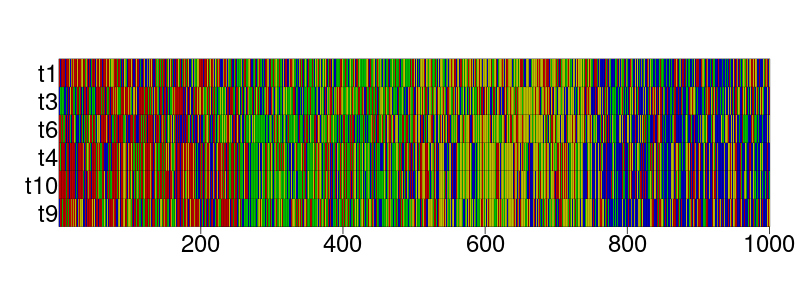
\includegraphics[height=0.25\textheight]{pirouette_example_30/example_30/true_alignment.png}
    };   
    \node[state] (CG) [below of = B, rectangle] {
      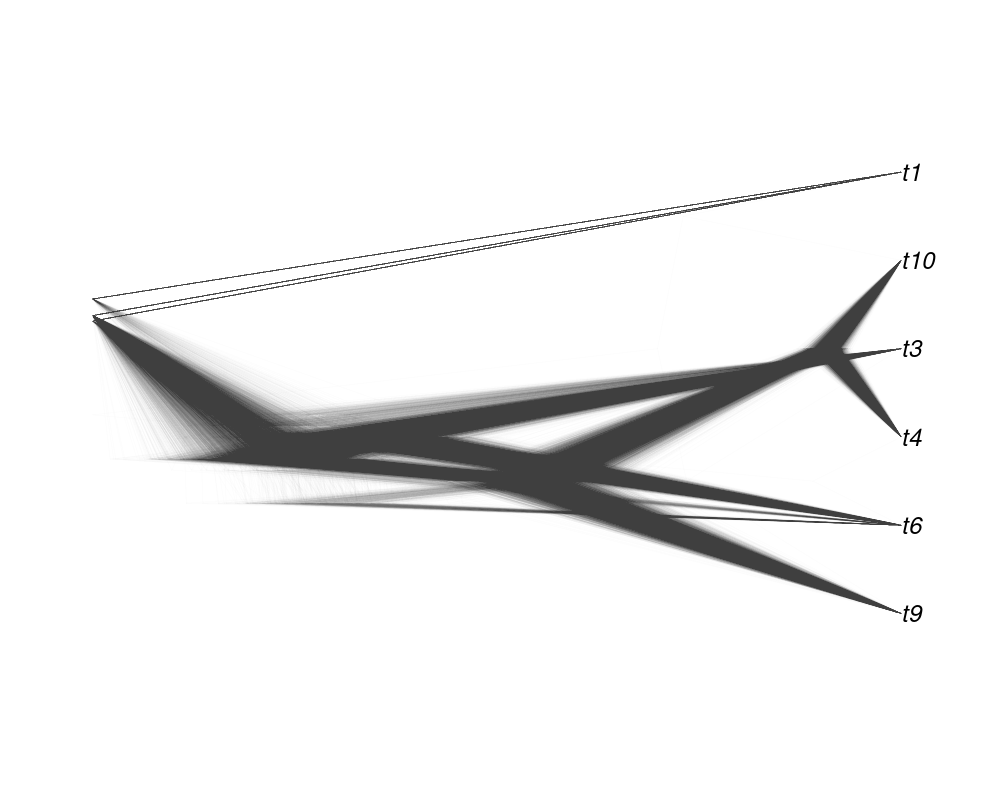
\includegraphics[height=0.3\textheight]{pirouette_example_30/example_30/true_posterior_gen.png}
    };   
    \node[state] (DG) [below of = CG, rectangle] {
      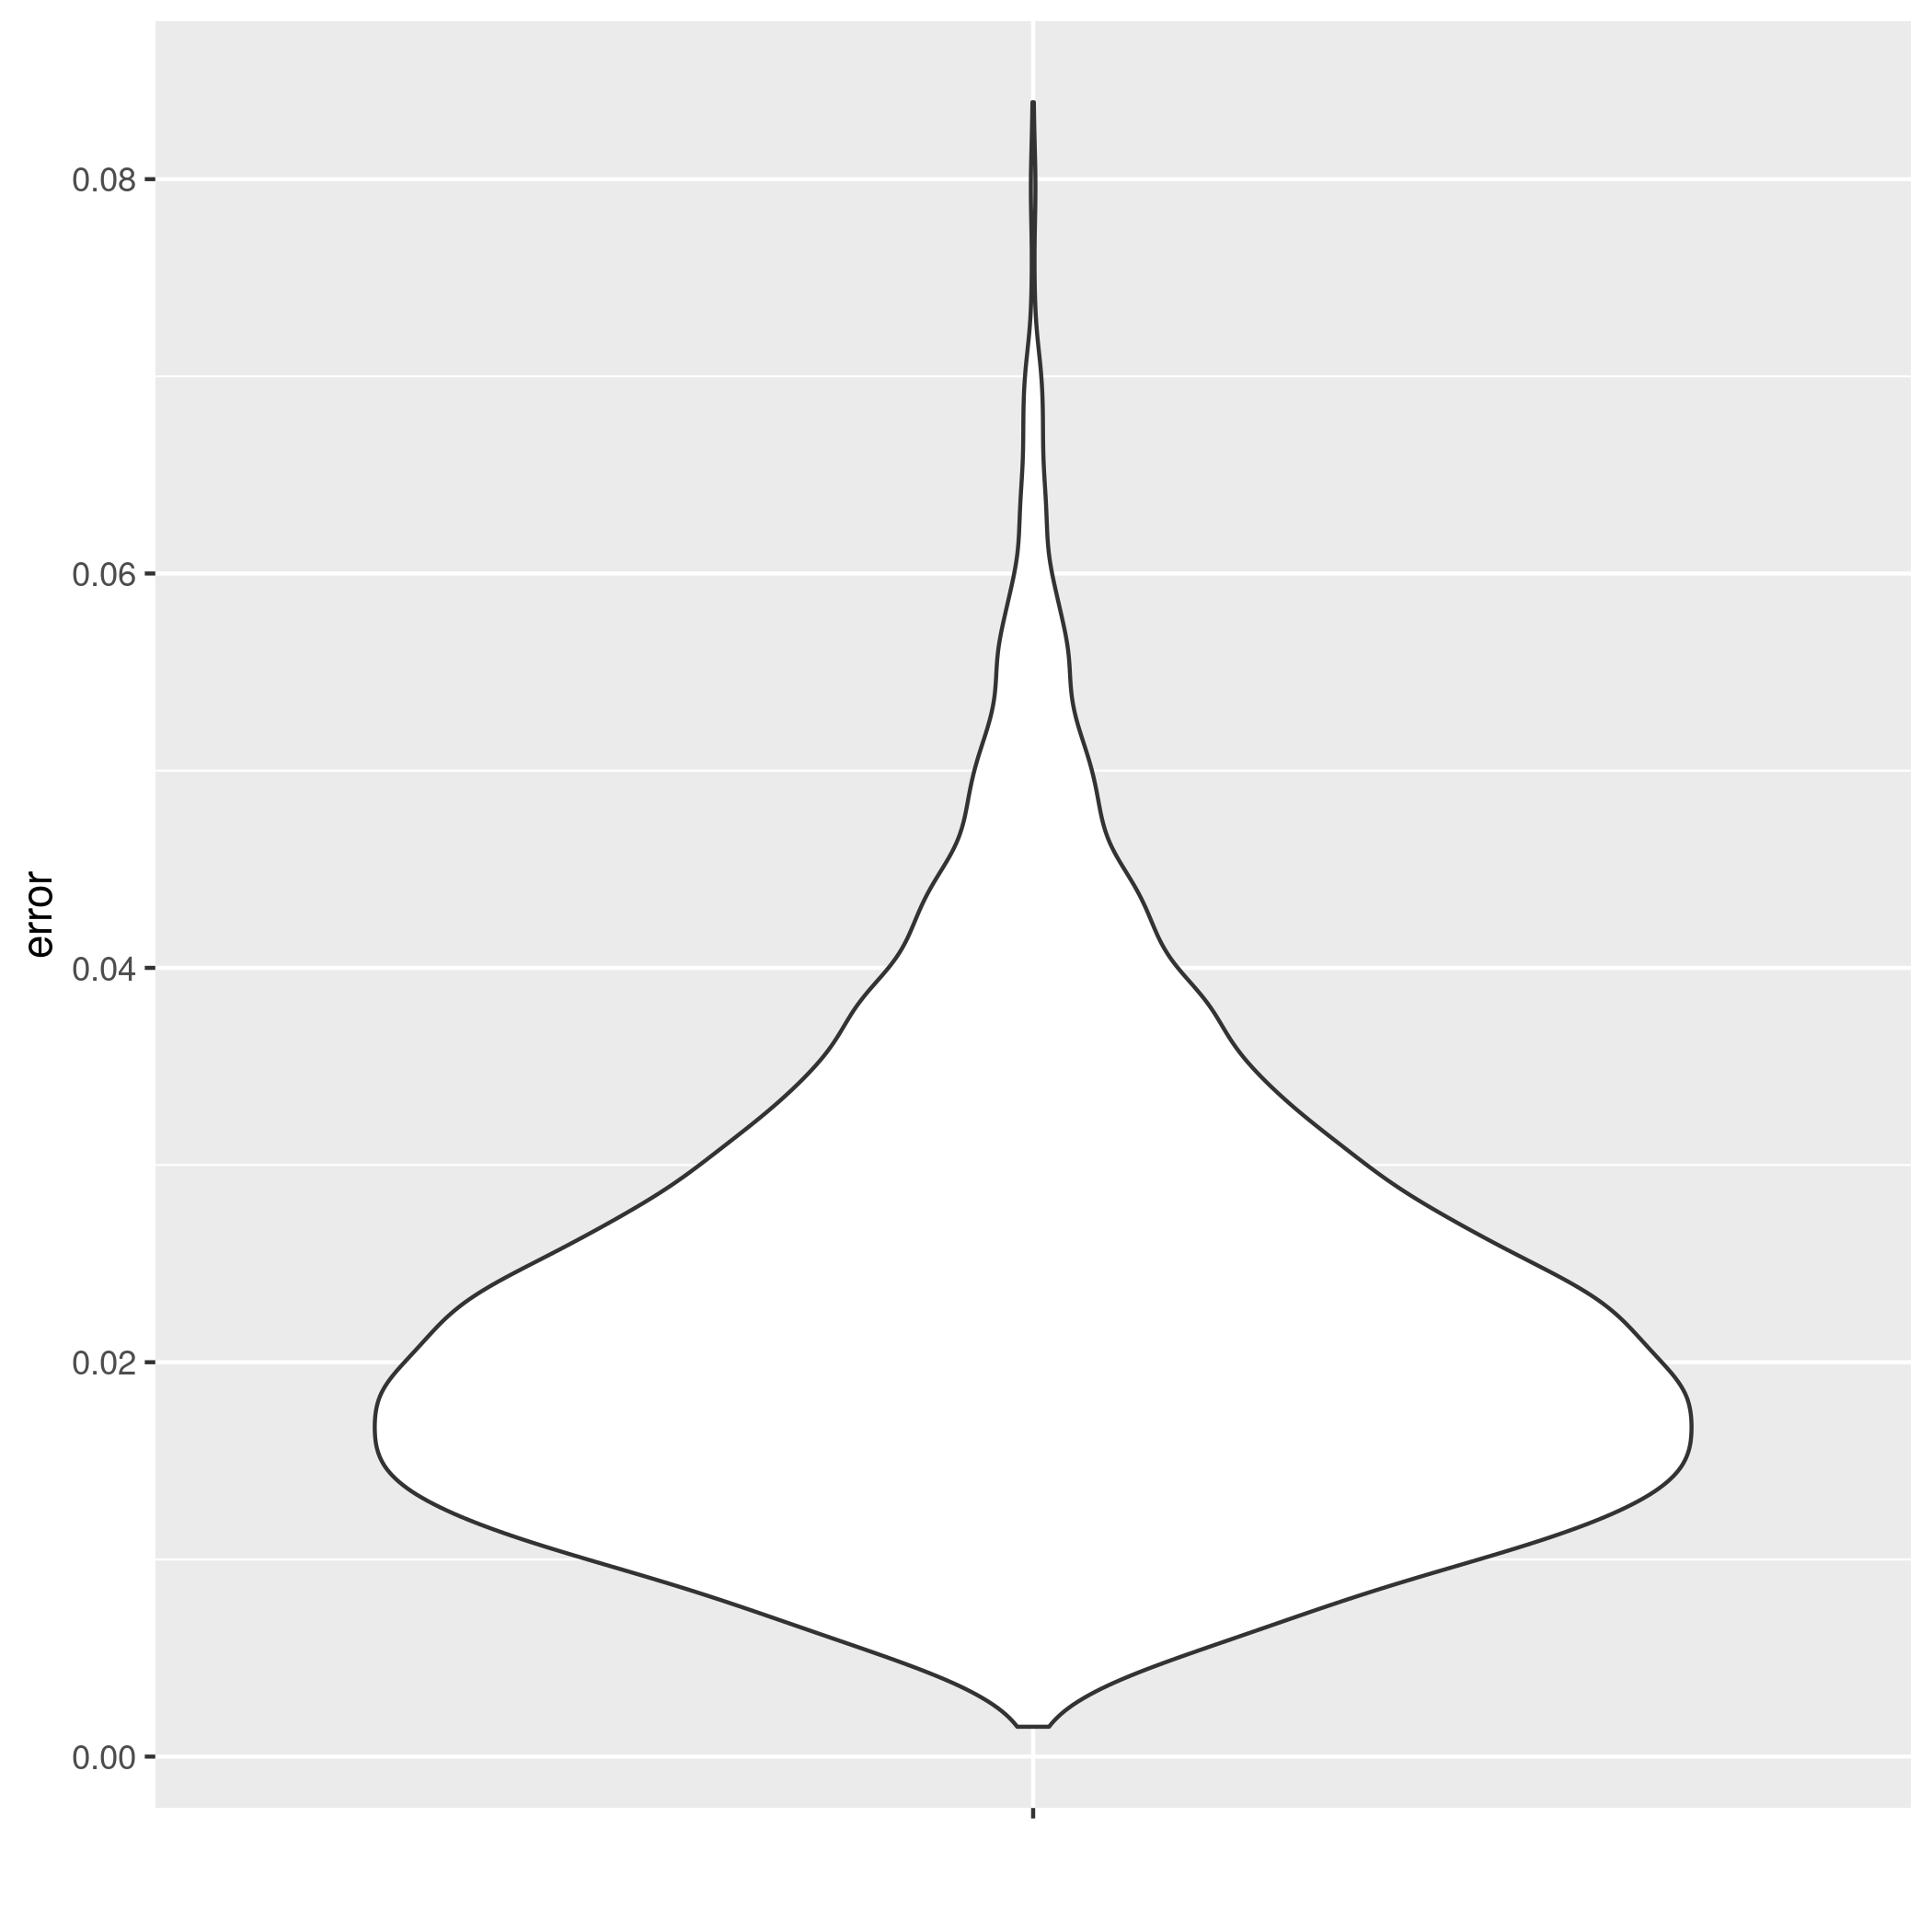
\includegraphics[height=0.3\textheight]{pirouette_example_30/example_30/true_error_violin_gen.png}
    };   
    \node[state] (CB) [right of = CG, rectangle] {
      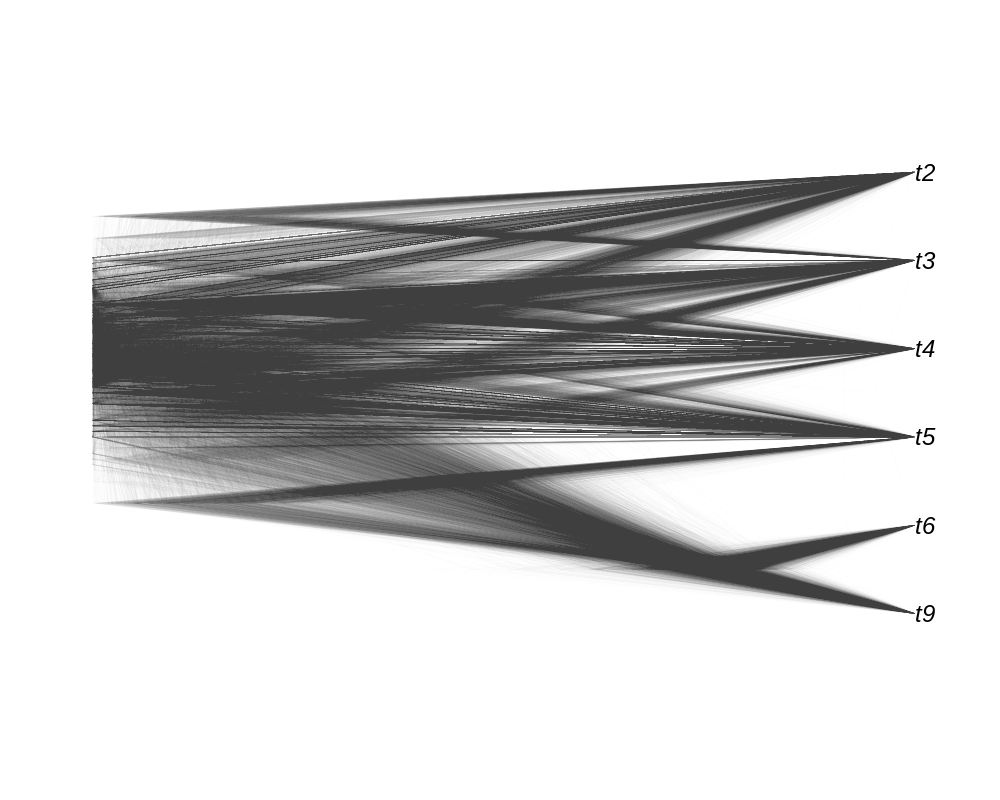
\includegraphics[height=0.3\textheight]{pirouette_example_30/example_30/true_posterior_best.png}
    };   
    \node[state] (DB) [below of = CB, rectangle] {
      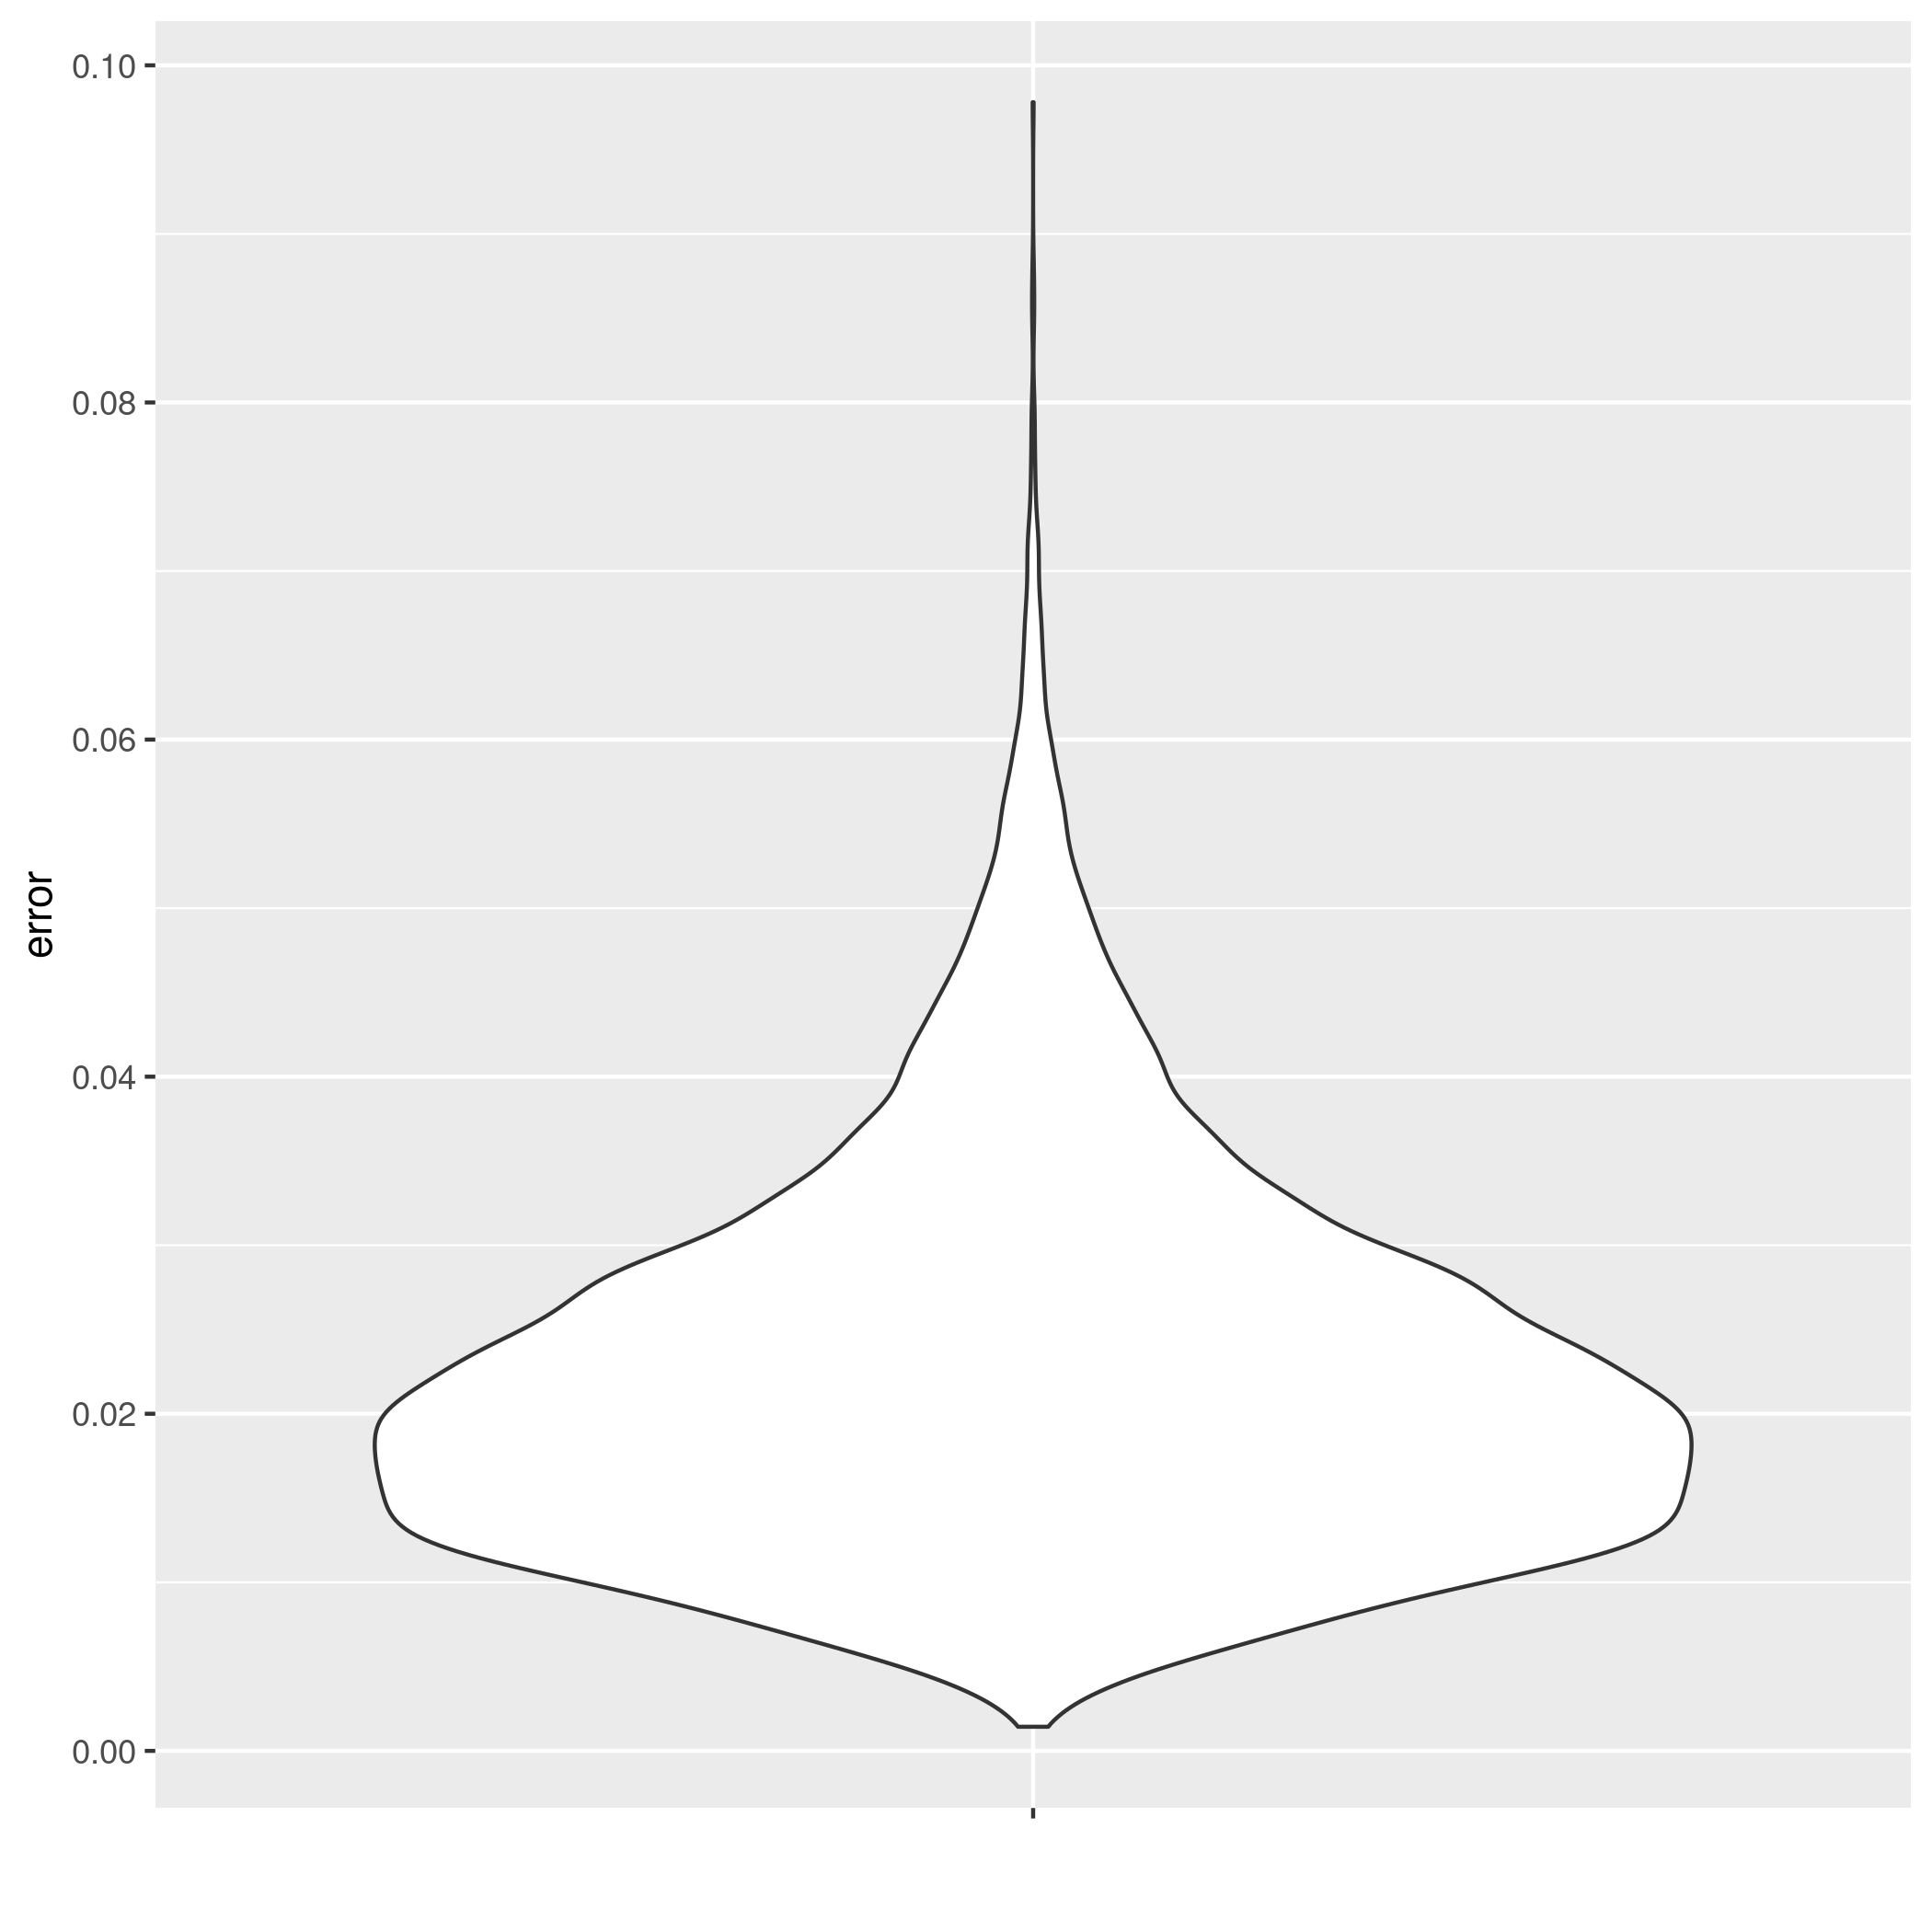
\includegraphics[height=0.3\textheight]{pirouette_example_30/example_30/true_error_violin_best.png}
    };   
    \node[state] (AT) [right of = A, rectangle, node distance=0.8\textheight] {
      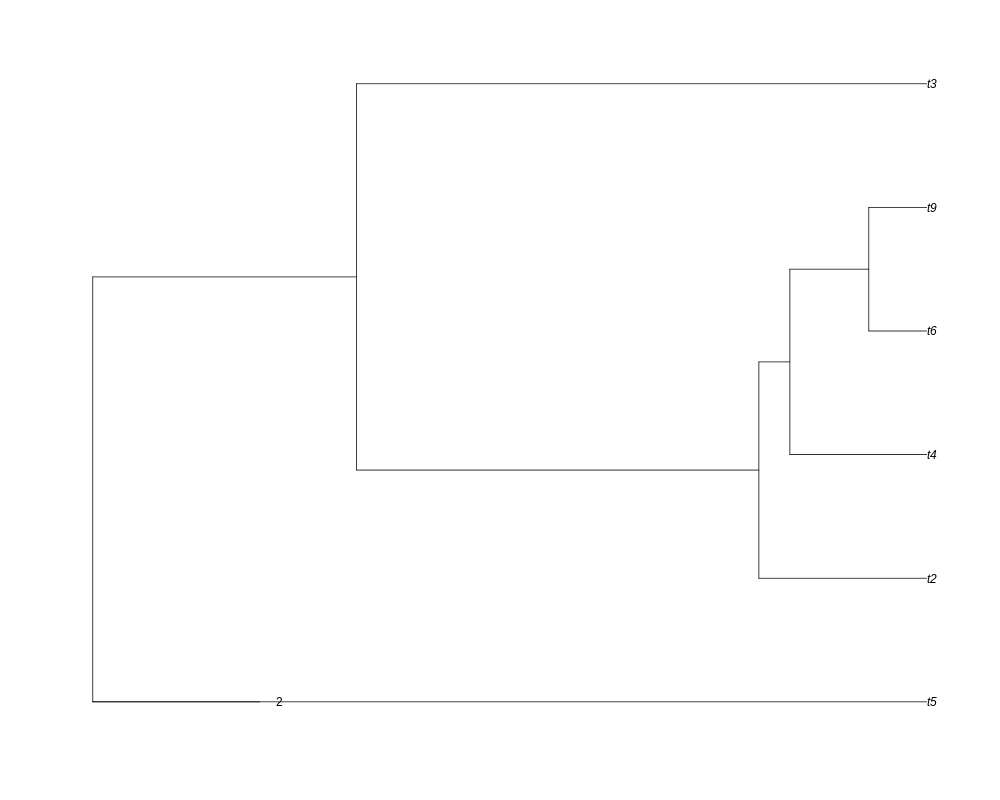
\includegraphics[height=0.4\textheight]{pirouette_example_30/example_30/twin_tree.png}
    };   
    \node[state] (BT) [below of = AT, rectangle] {
      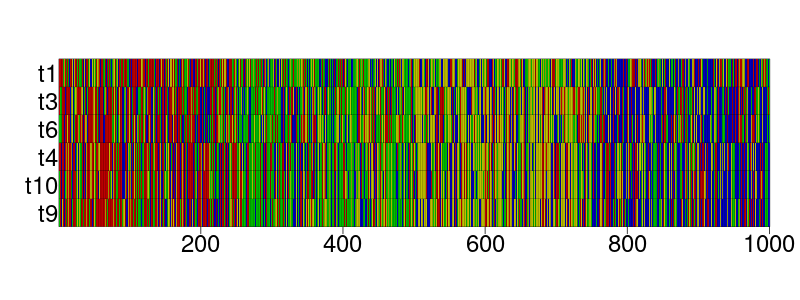
\includegraphics[height=0.25\textheight]{pirouette_example_30/example_30/twin_alignment.png}
    };   
    \node[state] (CTG) [right of = CB, rectangle] {
      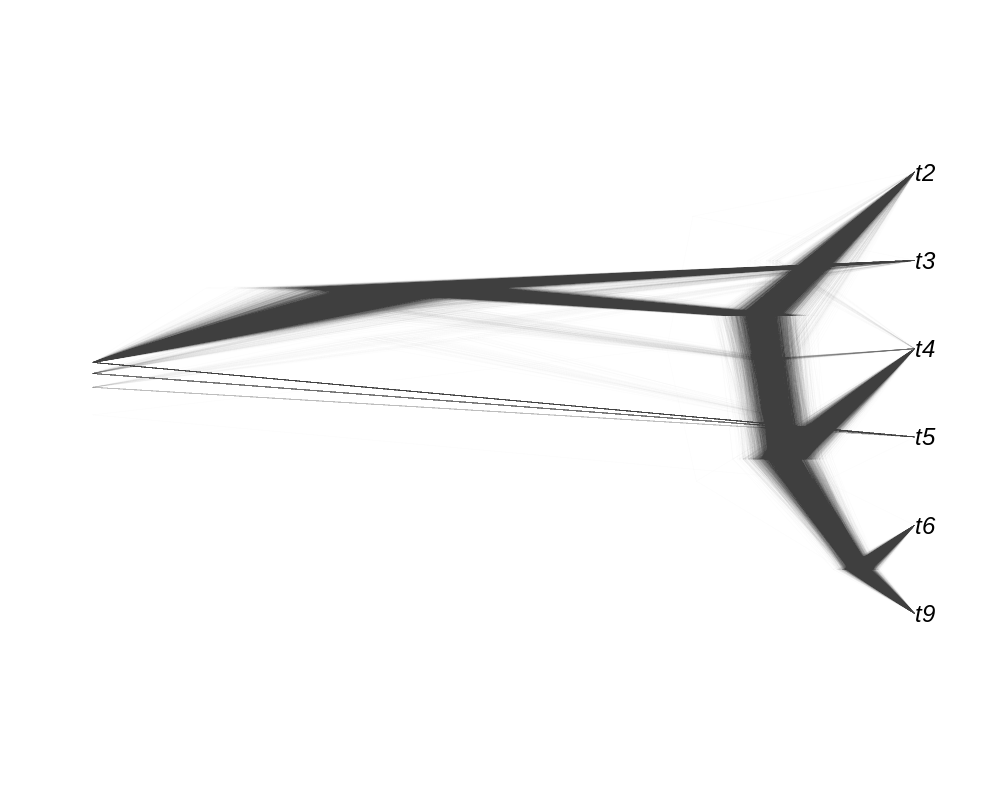
\includegraphics[height=0.3\textheight]{pirouette_example_30/example_30/twin_posterior_gen.png}
    };   
    \node[state] (DTG) [below of = CTG, rectangle] {
      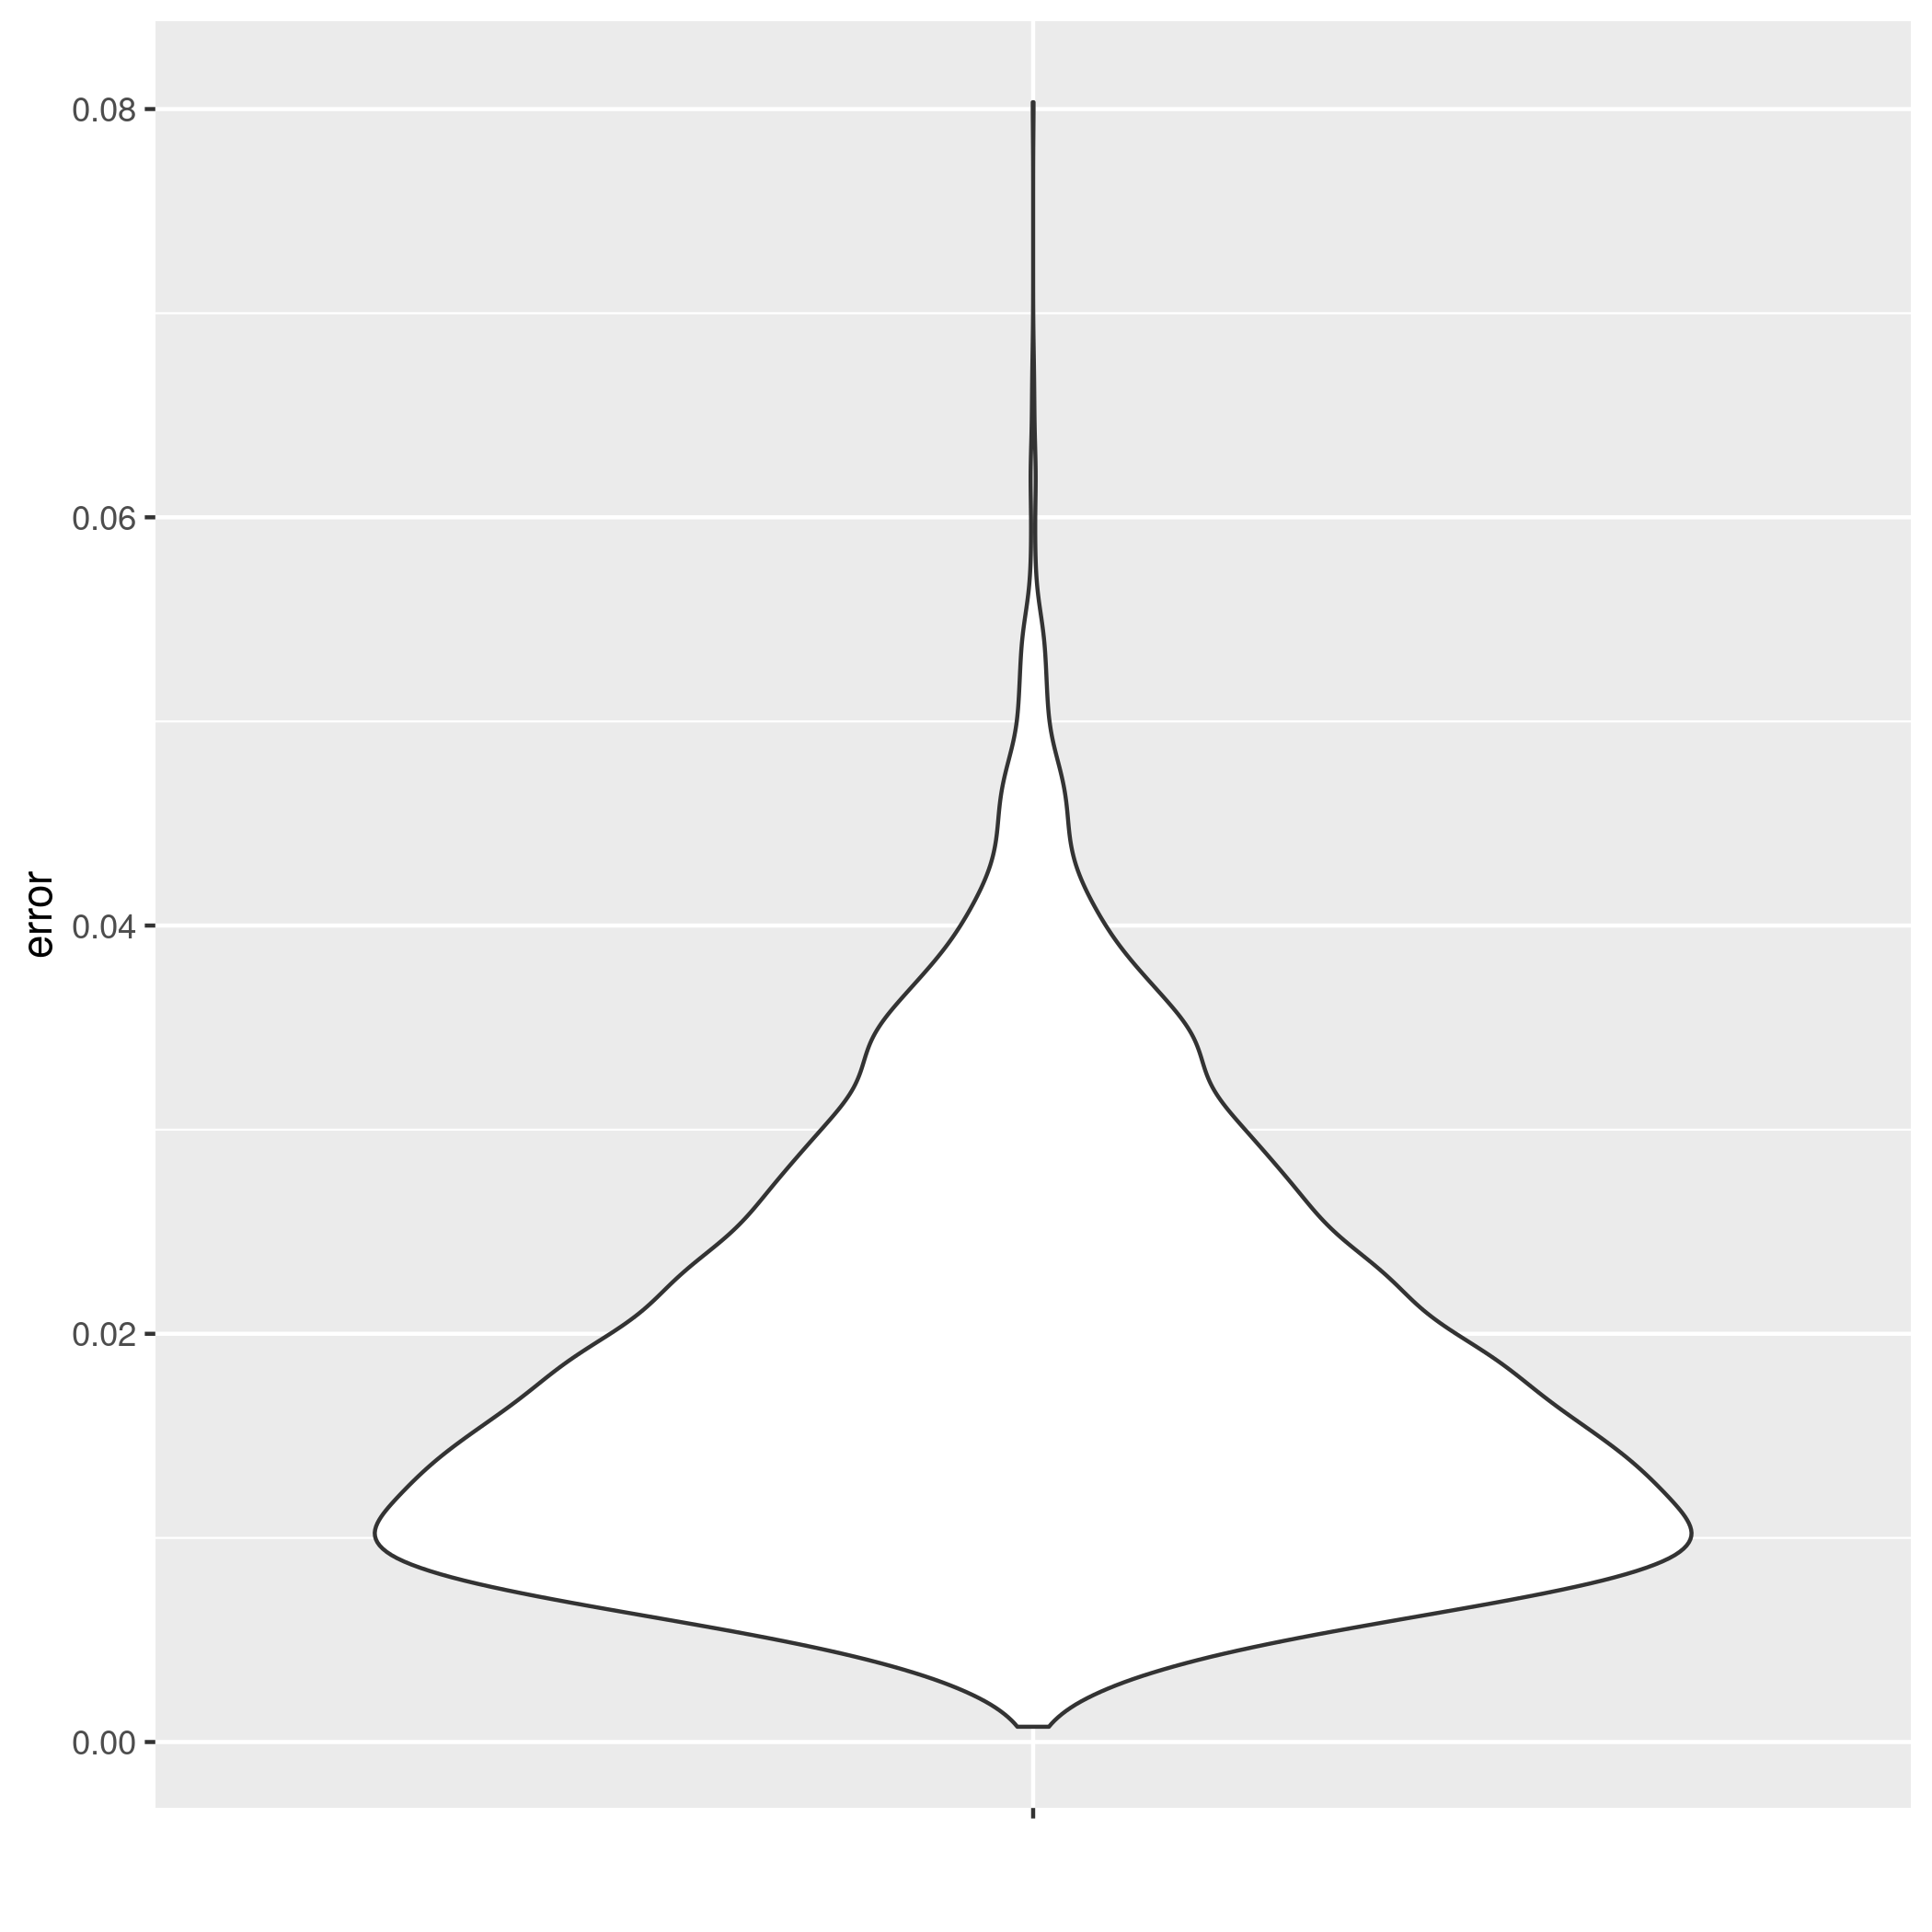
\includegraphics[height=0.3\textheight]{pirouette_example_30/example_30/twin_error_violin_gen.png}
    };   
    \node[state] (CTB) [right of = CTG, rectangle] {
      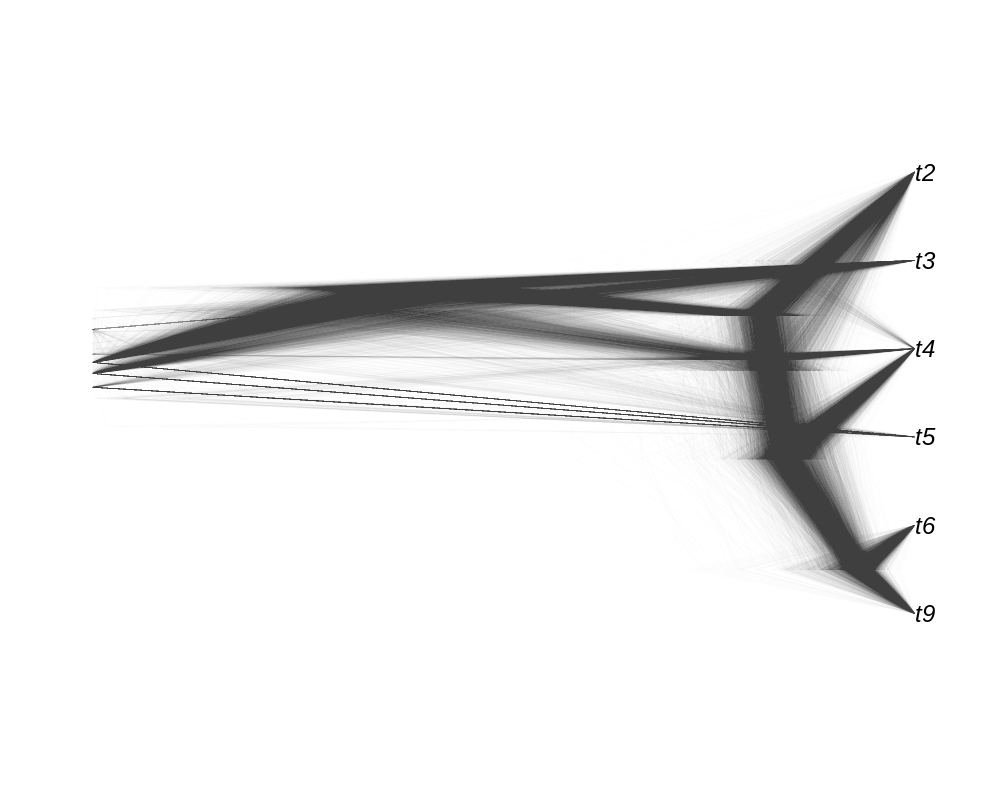
\includegraphics[height=0.3\textheight]{pirouette_example_30/example_30/twin_posterior_best.png}
    };   
    \node[state] (DTB) [below of = CTB, rectangle] {
      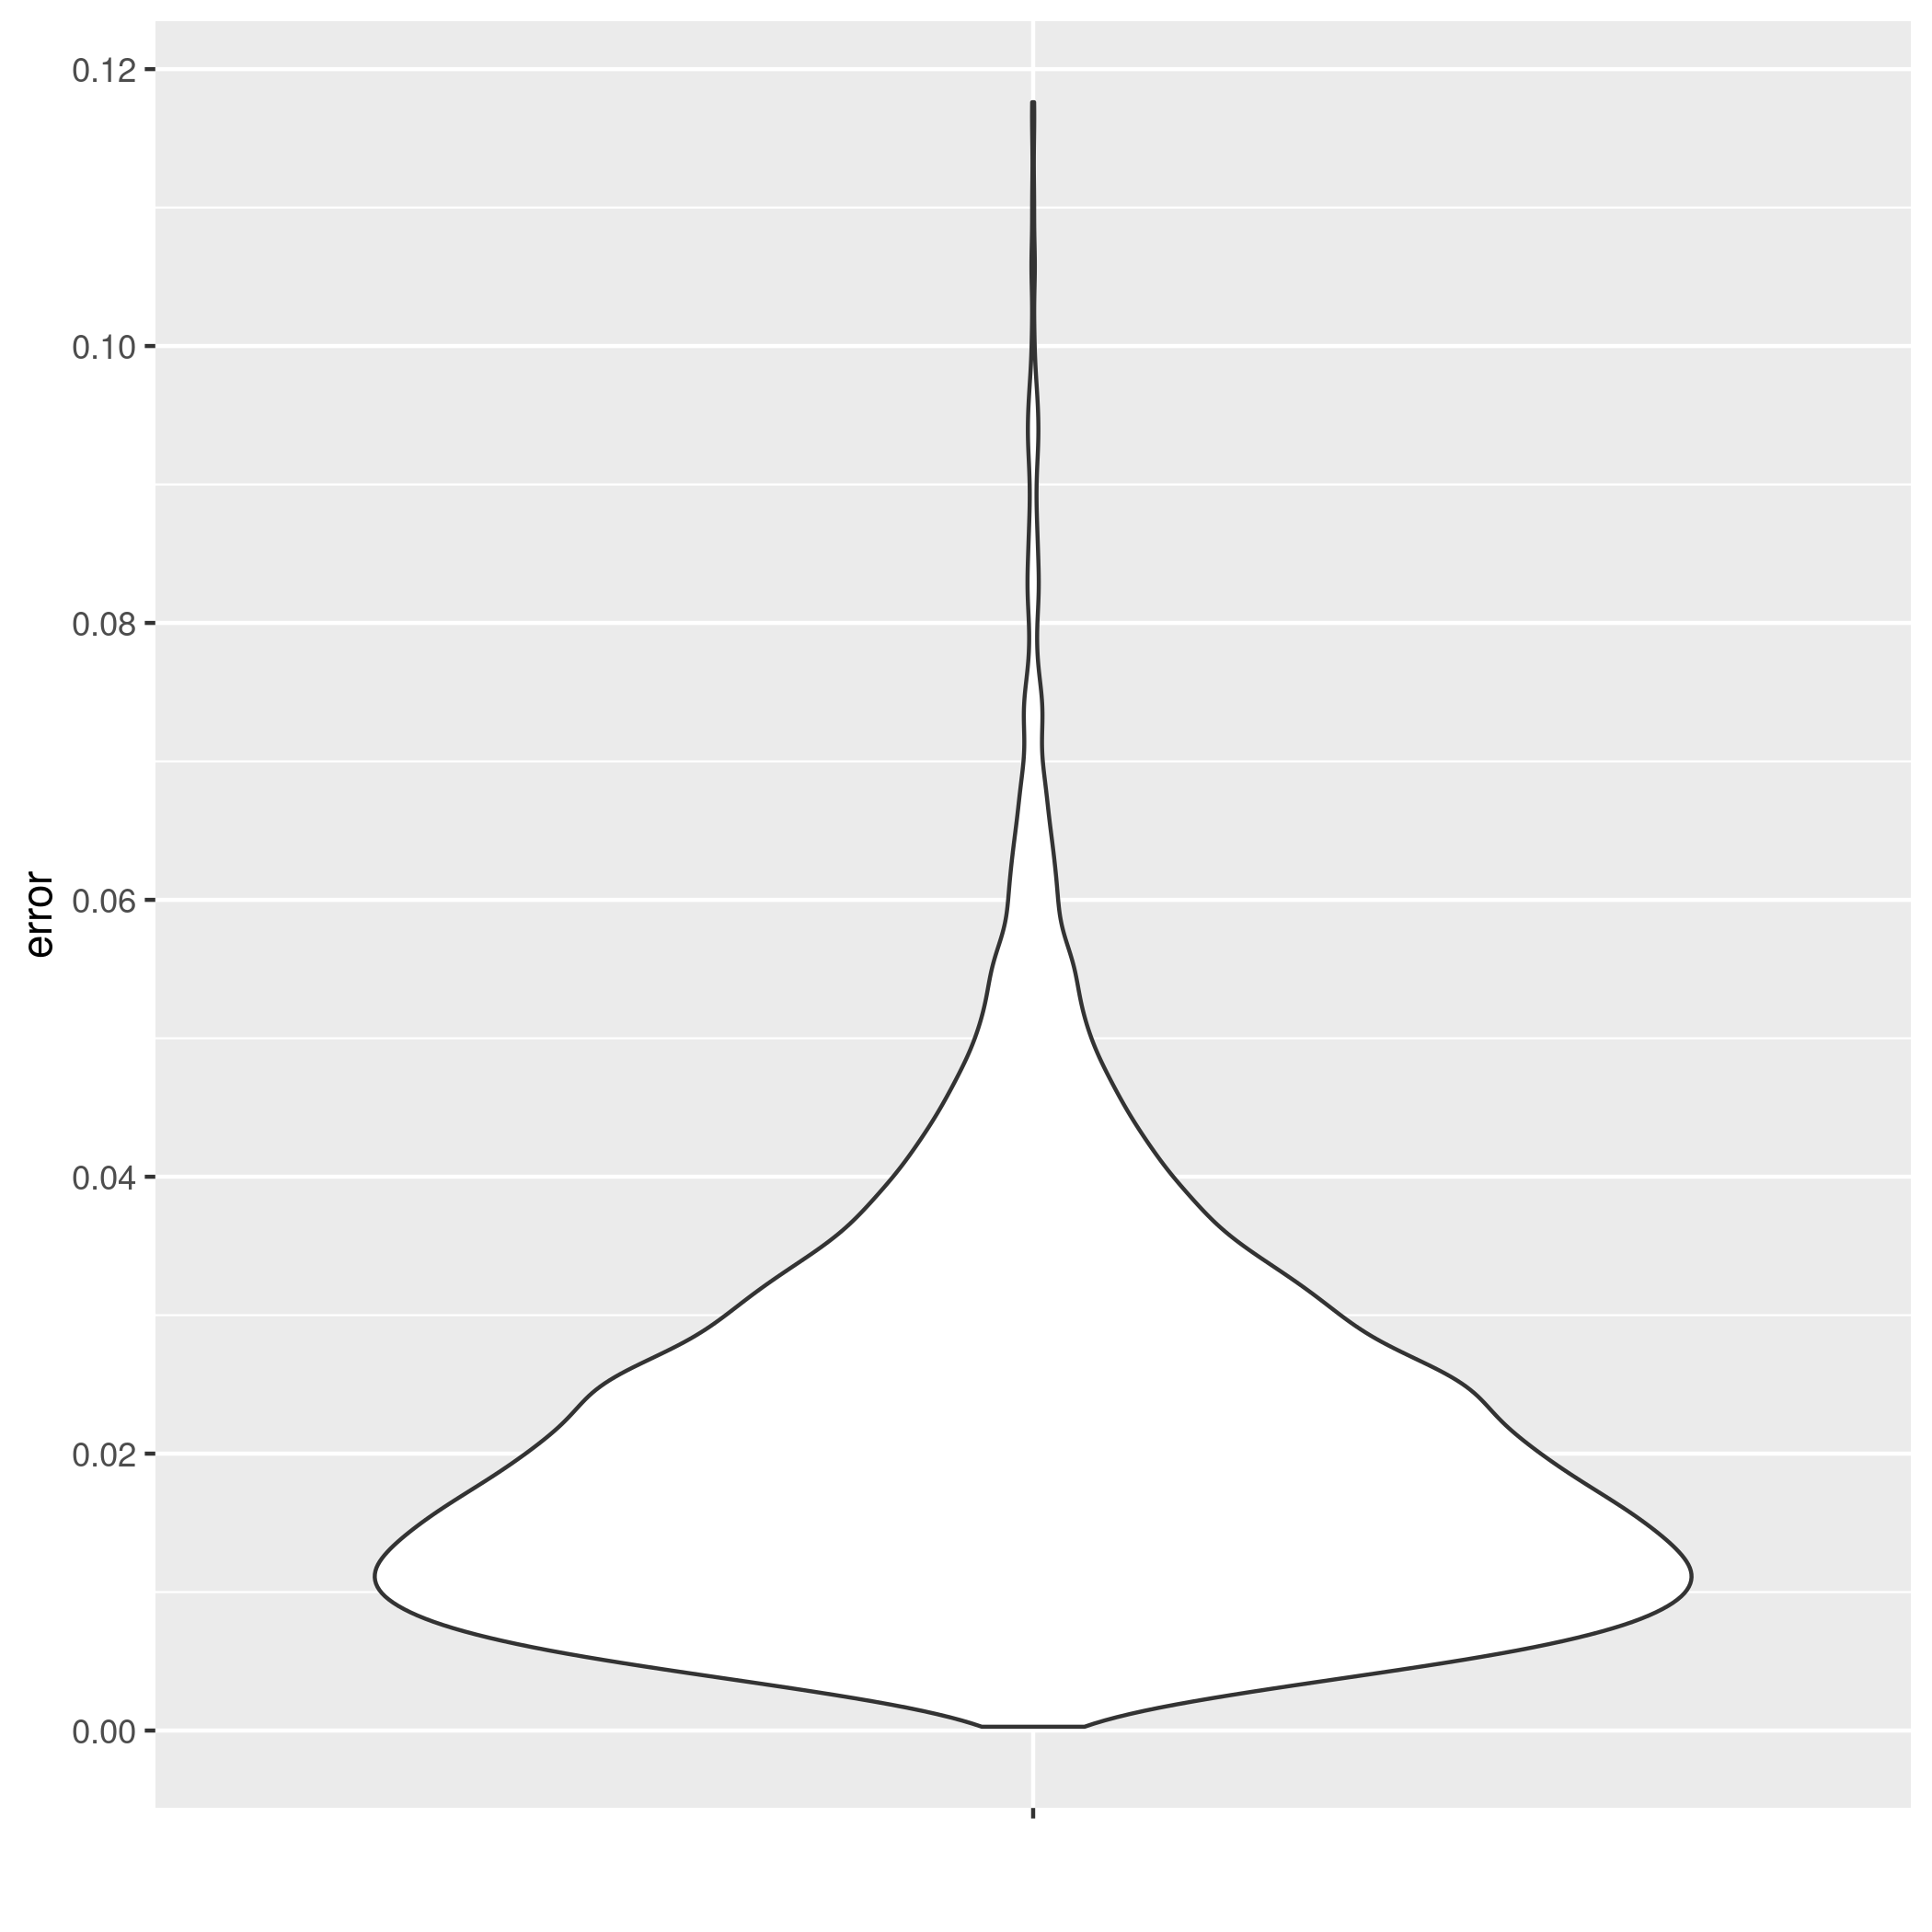
\includegraphics[height=0.3\textheight]{pirouette_example_30/example_30/twin_error_violin_best.png}
    };   
    \path 
      (O) edge [anchor = south] node {} (A)
      (A) edge [anchor = south] node {} (B)
      (B) edge [anchor = south] node {} (CG)
      (CG) edge [anchor = south] node {} (DG)
      (B) edge [anchor = south east] node {} (CB)
      (CB) edge [anchor = south] node {} (DB)
      (A) edge [anchor = east] node {} (AT)
      (AT) edge [anchor = south] node {} (BT)
      (BT) edge [anchor = south east] node {} (CTG)
      (CTG) edge [anchor = south] node {} (DTG)
      (BT) edge [anchor = south] node {} (CTB)
      (CTB) edge [anchor = south] node {} (DTB)
    ; 
    \end{tikzpicture}
  }
  \caption{Full pirouette pipeline, including comparison to baseline error. 
    The true tree (top left) is used to simulate an alignment. 
    From this alignment two posterior distributions of trees are created: 
    one using the generative model and another one using the inference model 
    with the highest marginal likelihood. 
    For each distribution of trees, a distribution of errors, 
    measured with the nLTT statistic, 
    between the posterior trees and the main trees is drawn. 
    From the true tree also a twin tree is created (right side of the figure)
    which follows the same pipeline, 
    leading to two additional error distributions to use as baseline errors.}
  \label{fig:example_30_full_pipeline}
\end{figure}
%%%%%%%%%%%%%%%%%%%%%%%%%%%%%%%%%%%%%%%%%%%%%%%%%%%%%%%%%%%%%%%%%%%%%%%%%%%%%%%%

To assess if the results of the inference are meaningful one important 
parameter is the Effective Sample Size (ESS). This quantity describes how 
many independent trees are sampled from the posterior distributions. 
For reliable results it is good practice to have at 
least $ESS = 200$ (see 
\begin{sloppypar}
  \url{https://beast.community/ess_tutorial}).
\end{sloppypar}
In the following we present the ESS for the posterior distributions of 
the 4 cases shown in Fig. \ref{fig:example_30_full_pipeline}.

The ESSes of the 'true' pipeline for the generative model
are shown in Table \ref{tab:esses_gen}.
From the estimated parameters, one can deduce that
the JC69 nucleotide substitution model was used (no
estimated parameter needed), a strict clock model was 
used (again, no parameter needed to be estimated)
and a Yule tree prior is used ('Yule model' and 'birthRate' are estimated).
Note that although the actual true tree is created by a DD process, 
the default and standard Yule tree model is used as the closest
standard tree model.

\input{pirouette_example_30/example_30/esses_gen.latex}

\newpage

The ESSes of the 'twin' pipeline for the generative model
are shown in Table \ref{tab:esses_twin_gen}.
Note that the generative inference model is 
re-used (which assumes a Yule tree model) in the inference, 
where the twin tree is actually created using a BD process,
which is the default.

\input{pirouette_example_30/example_30/esses_twin_gen.latex}

\newpage

The ESSes of the 'true' pipeline for the best candidate model
are shown in Table \ref{tab:esses_best}. 
From the names of the estimated parameters, it is clear that
the best candidate model has had a TN93 nucleotide substitution 
model (due to 'kappa1', 'kappa2', 'freqParameter.1', 
'freqParameter.2', 'freqParameter.3', 'freqParameter.4')
a strict clock (no parameter needed to be estimated) and a BD 
model ('BirthDeath', 'BDBirthRate' and 'BDDeathRate').

\input{pirouette_example_30/example_30/esses_best.latex}

\newpage

The ESSes of the 'twin' pipeline for the best candidate model
are shown in Table \ref{tab:esses_twin_best}.

From the names of the estimated parameters, it is clear that
the best candidate model for the twin tree
is JC69 nucleotide substitution 
model (no parameter needed to be estimated),
a strict clock (no parameter needed to be estimated) and a BD 
model ('BirthDate', 'BDBirthRate' and 'BDDeathRate').
Note that this matches the actual process of how the twin tree
and twin alignment are generated.

\input{pirouette_example_30/example_30/esses_twin_best.latex}

\newpage

The marginal likelihood (or evidence) data for the model comparison
performed in the 'true' pipeline is shown in Table \ref{tab:evidence_true}.
The best (that is, the one with the highest model weight)
candidate model assumes a TN93 nucleotide substitution model,
a strict clock and a BD model.

\input{pirouette_example_30/example_30/evidence_true.latex}

\newpage

The marginal likelihood (or evidence) data for model comparison
performed in the 'twin' pipeline is shown in Table \ref{tab:evidence_twin}.
The best (that is, the one with the highest model weight)
candidate model assumes a JC69 nucleotide substitution model,
a strict clock and a BD model.
Note that this matches the actual process of how the twin tree
and twin alignment are generated.

\input{pirouette_example_30/example_30/evidence_twin.latex}

\newpage

%%%%%%%%%%%%%%%%%%%%%%%%%%%%%%%%%%%%%%%%%%%%%%%%%%%%%%%%%%%%%%%%%%%%%%%%%%%%%%%%
\subsection{Using a distribution of trees}
\label{subsec:distribution}
%%%%%%%%%%%%%%%%%%%%%%%%%%%%%%%%%%%%%%%%%%%%%%%%%%%%%%%%%%%%%%%%%%%%%%%%%%%%%%%%

This subsection extends the main example, by using multiple (instead of
one) trees. These trees are produced by running a DD tree simulation
with the same parameters as the main example.

\begin{figure}[H]
  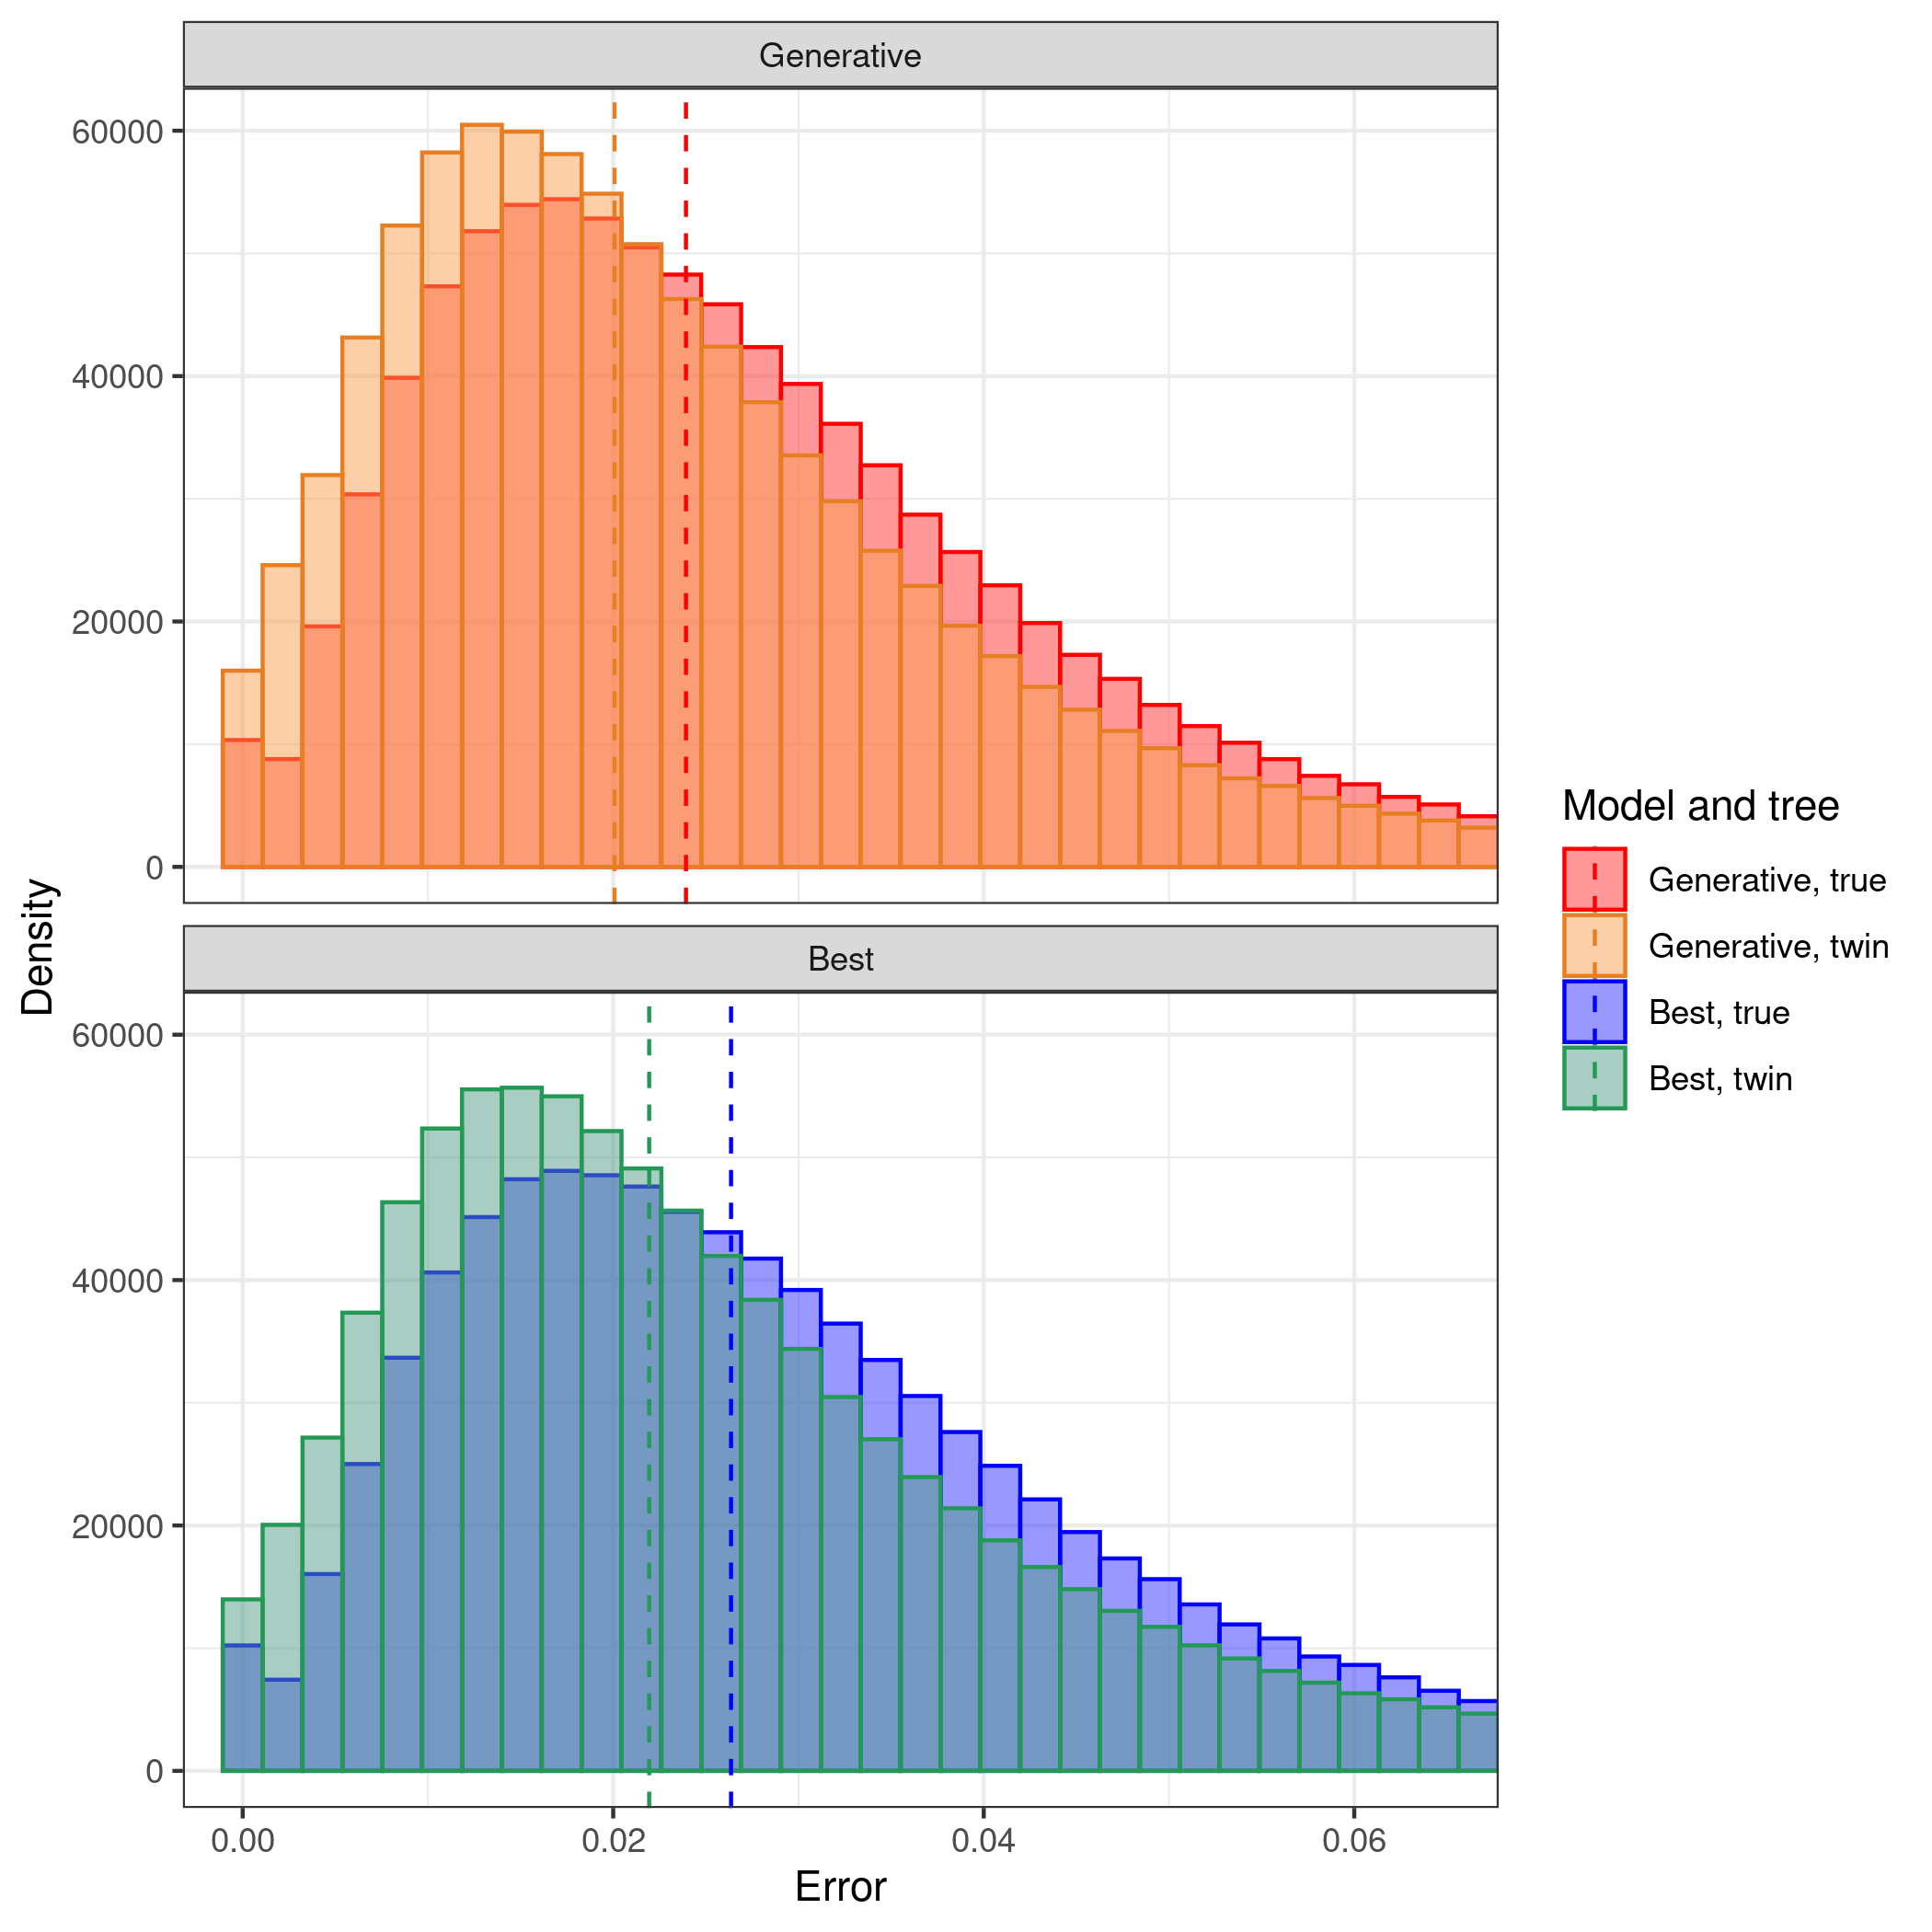
\includegraphics[width=0.98\textwidth]{pirouette_example_28/errors.png}
  \caption{
    Aggregate error distributions, 
    similar to Fig. \ref{fig:example_30} for the main example, 
    but now for a collection of 100 replicate trees. 
    For each setting (true generative, true best candidate, 
    twin generative and twin best candidate), the resulting errors 
    from each replicate pipeline have been merged into a single distribution. 
    This took 2.7 days (wall clock time) to compute.
  }
  \label{fig:replicate_trees}
\end{figure}

\new{
  The resulting error distributions are shown in Fig. \ref{fig:replicate_trees}. 
  We present results for cases where (1) the generative model has been used 
  or (2) the model with highest evidence has been selected for the inference.
  From the plots we can see that in both cases the two distributions 
  (true and twin) are mostly overlapping, but not everywhere.
  This suggests that the inference 
  models that have been used can to a reasonable extent capture in an accurate way 
  the features of the diversity-dependent tree prior used to simulate 
  the original trees. 
}

The code to reproduce Fig. \ref{fig:replicate_trees} can be found at  
\begin{sloppypar}
  \url{https://github.com/richelbilderbeek/pirouette_example_28}.
\end{sloppypar}

\newpage

%%%%%%%%%%%%%%%%%%%%%%%%%%%%%%%%%%%%%%%%%%%%%%%%%%%%%%%%%%%%%%%%%%%%%%%%%%%%%%%%
\subsection{The effect of the number of taxa}
\label{subsec:n_taxa}
%%%%%%%%%%%%%%%%%%%%%%%%%%%%%%%%%%%%%%%%%%%%%%%%%%%%%%%%%%%%%%%%%%%%%%%%%%%%%%%%

The main example uses 6 taxa. Here we show the same results as the main example,
except for a varying number of taxa. We did so, by setting the DD model's
carrying capacity to the desired number of taxa.

\begin{figure}[H]
  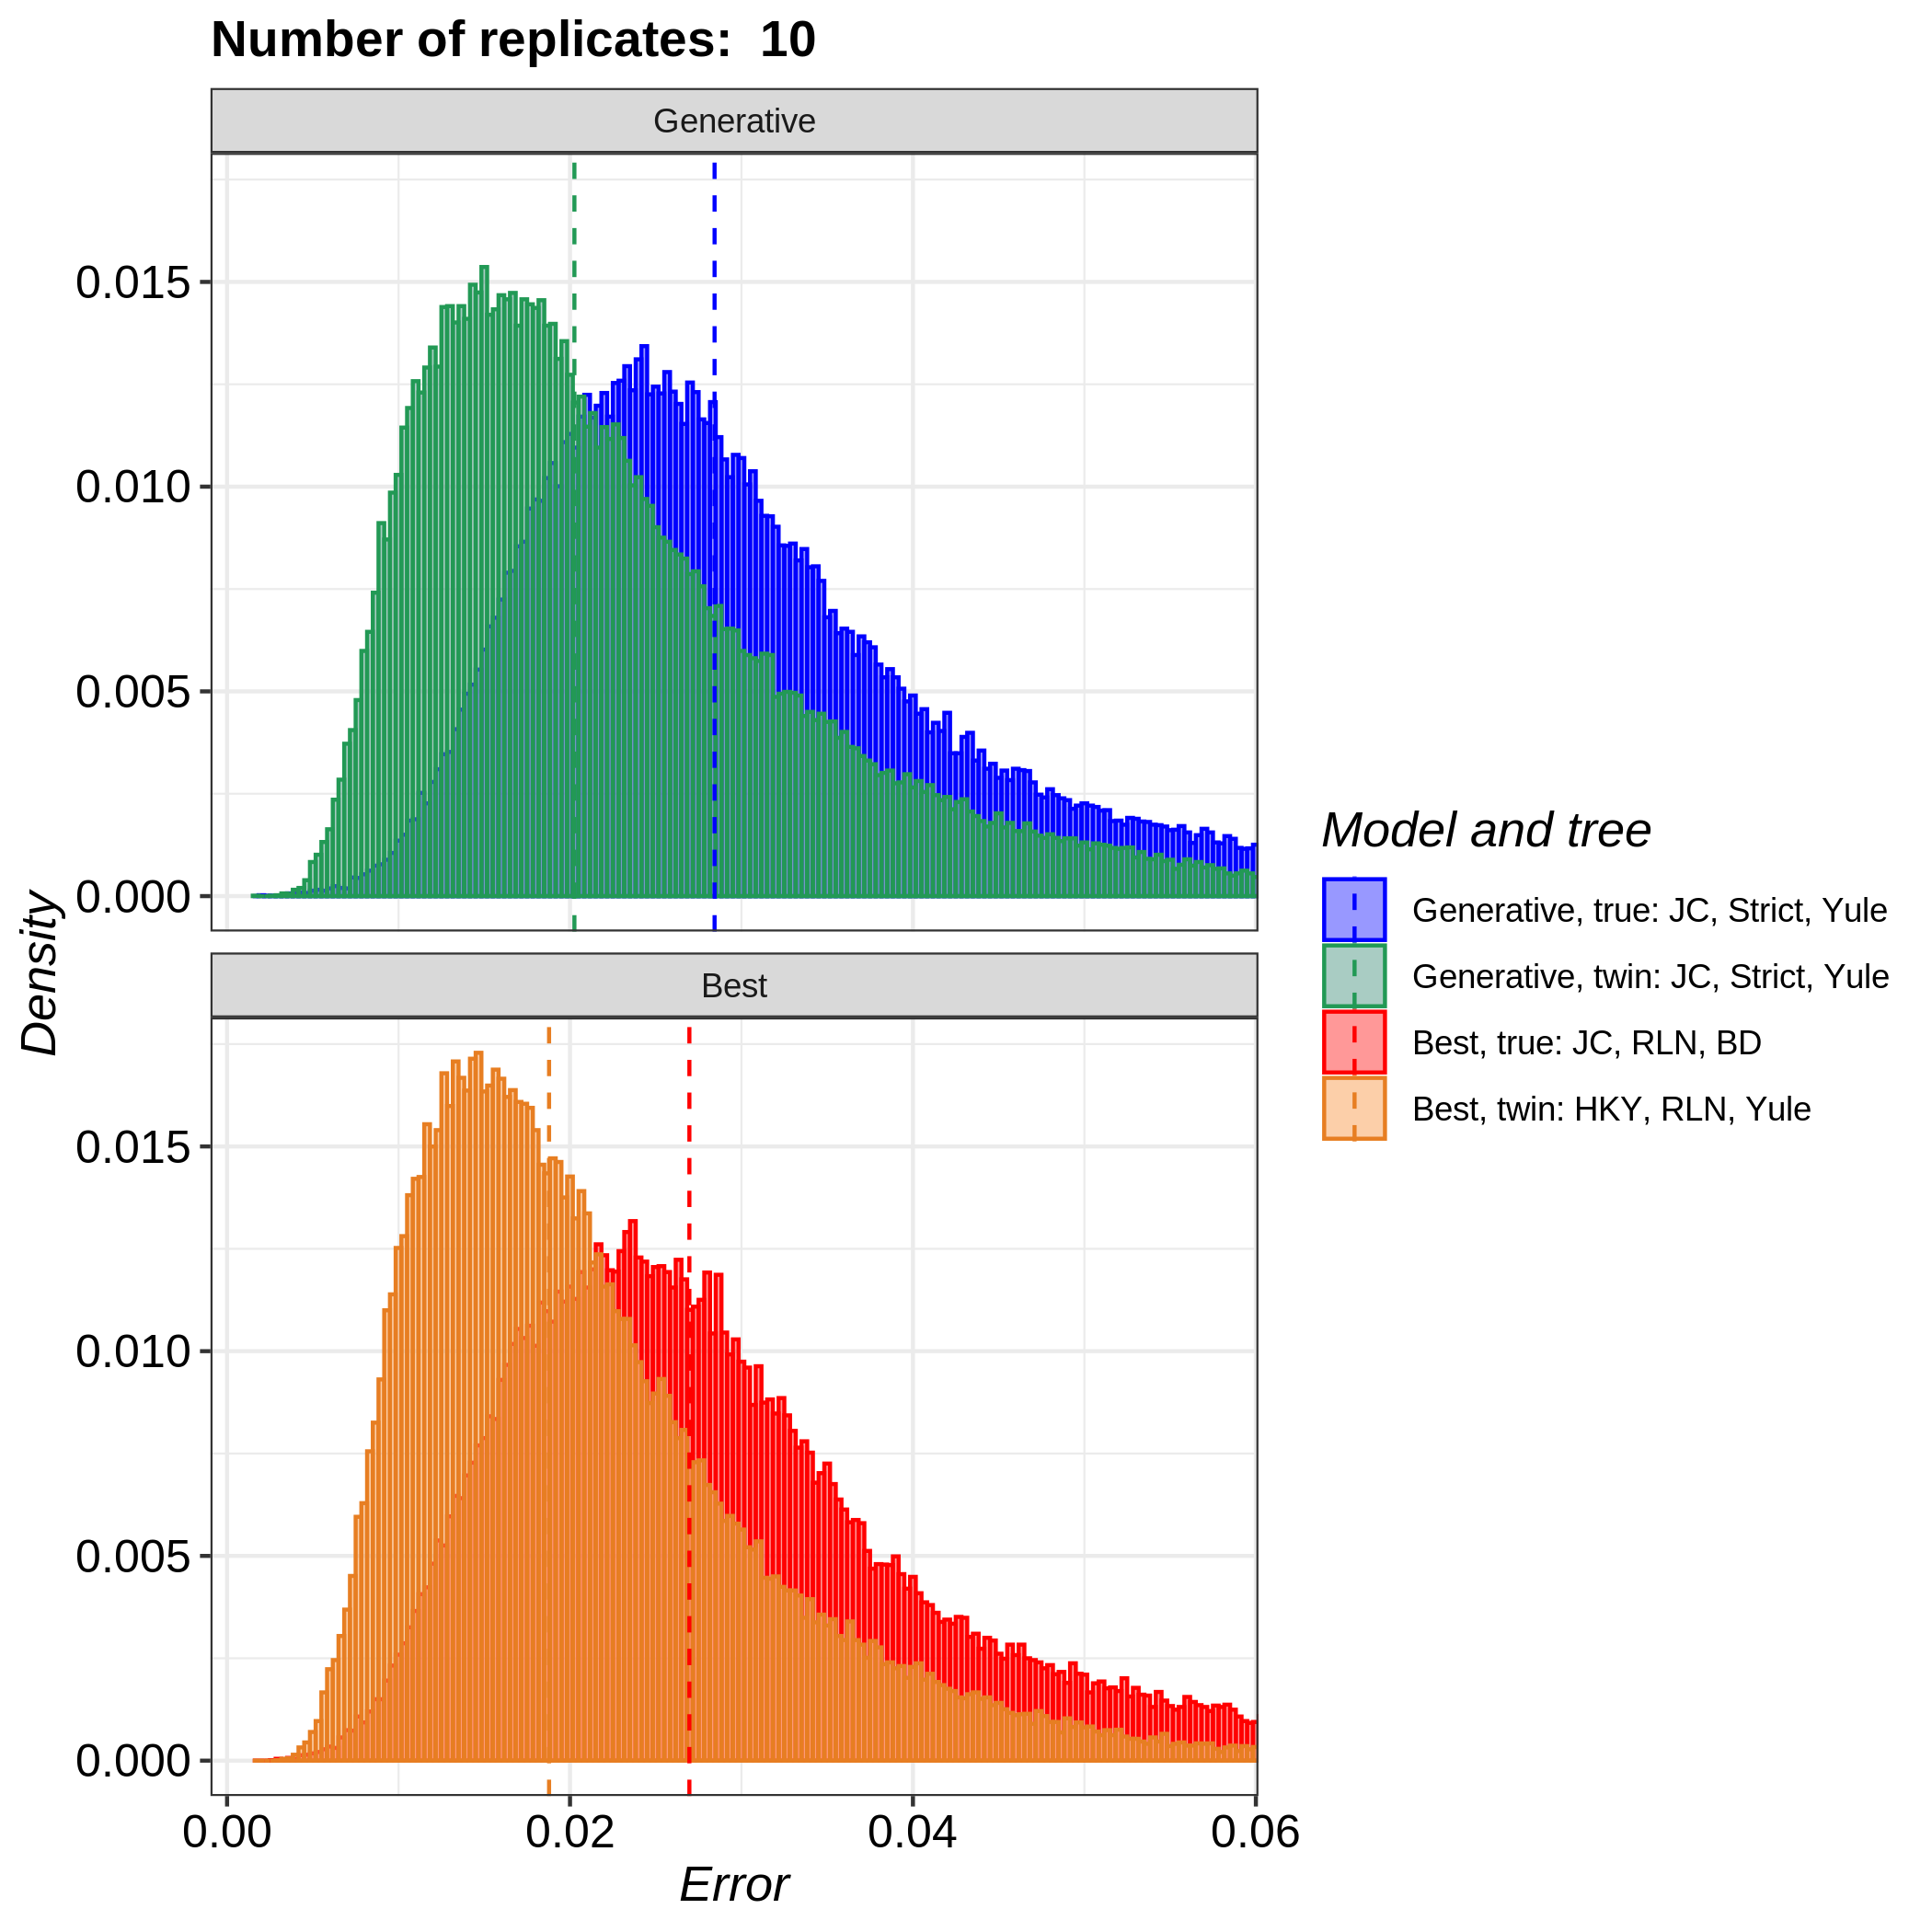
\includegraphics[width=0.98\textwidth]{pirouette_example_32/errors.png}
  \caption{Aggregate error distributions for 100 replicates. Here each true tree has 12 taxa. This took 6.0 days (wall clock time) to compute.}
  \label{fig:example_12_taxa}
\end{figure}

\begin{figure}[H]
  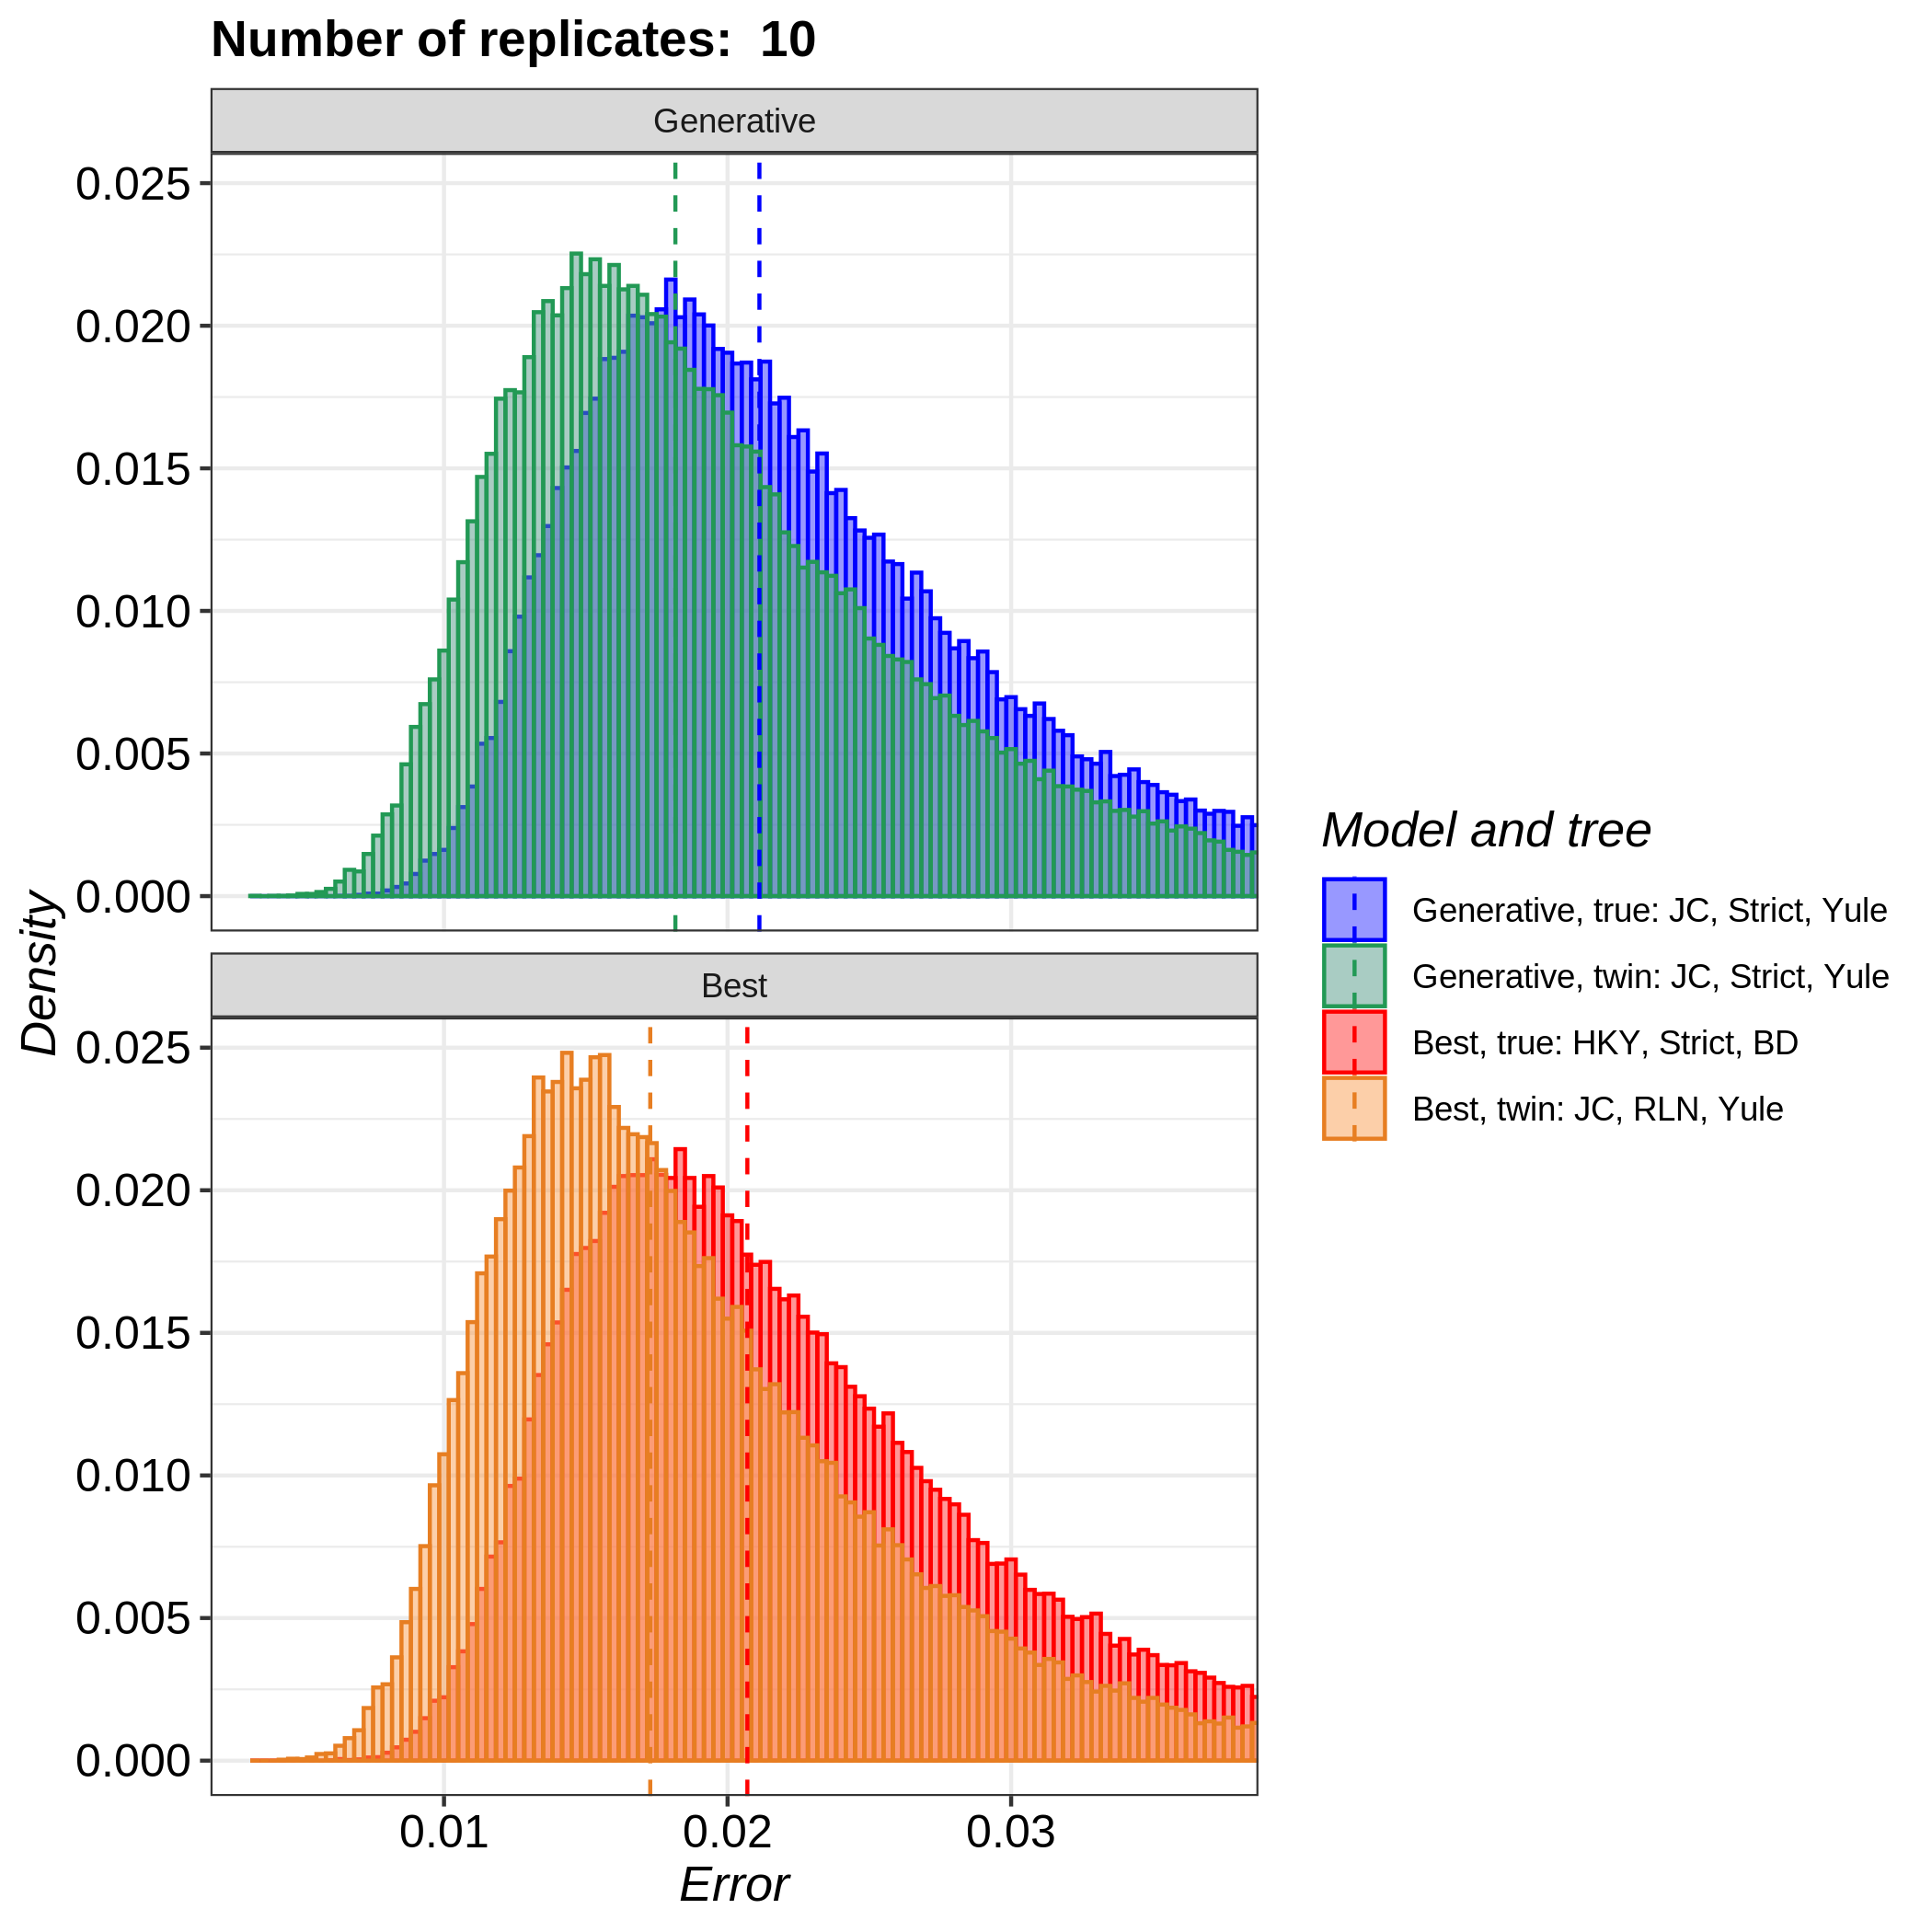
\includegraphics[width=0.98\textwidth]{pirouette_example_33/errors.png}
  \caption{Aggregate error distributions for 100 replicates. Here each true tree has 24 taxa. This took 9.8 days (wall clock time) to compute.}
  \label{fig:example_24_taxa}
\end{figure}

\begin{figure}[H]
  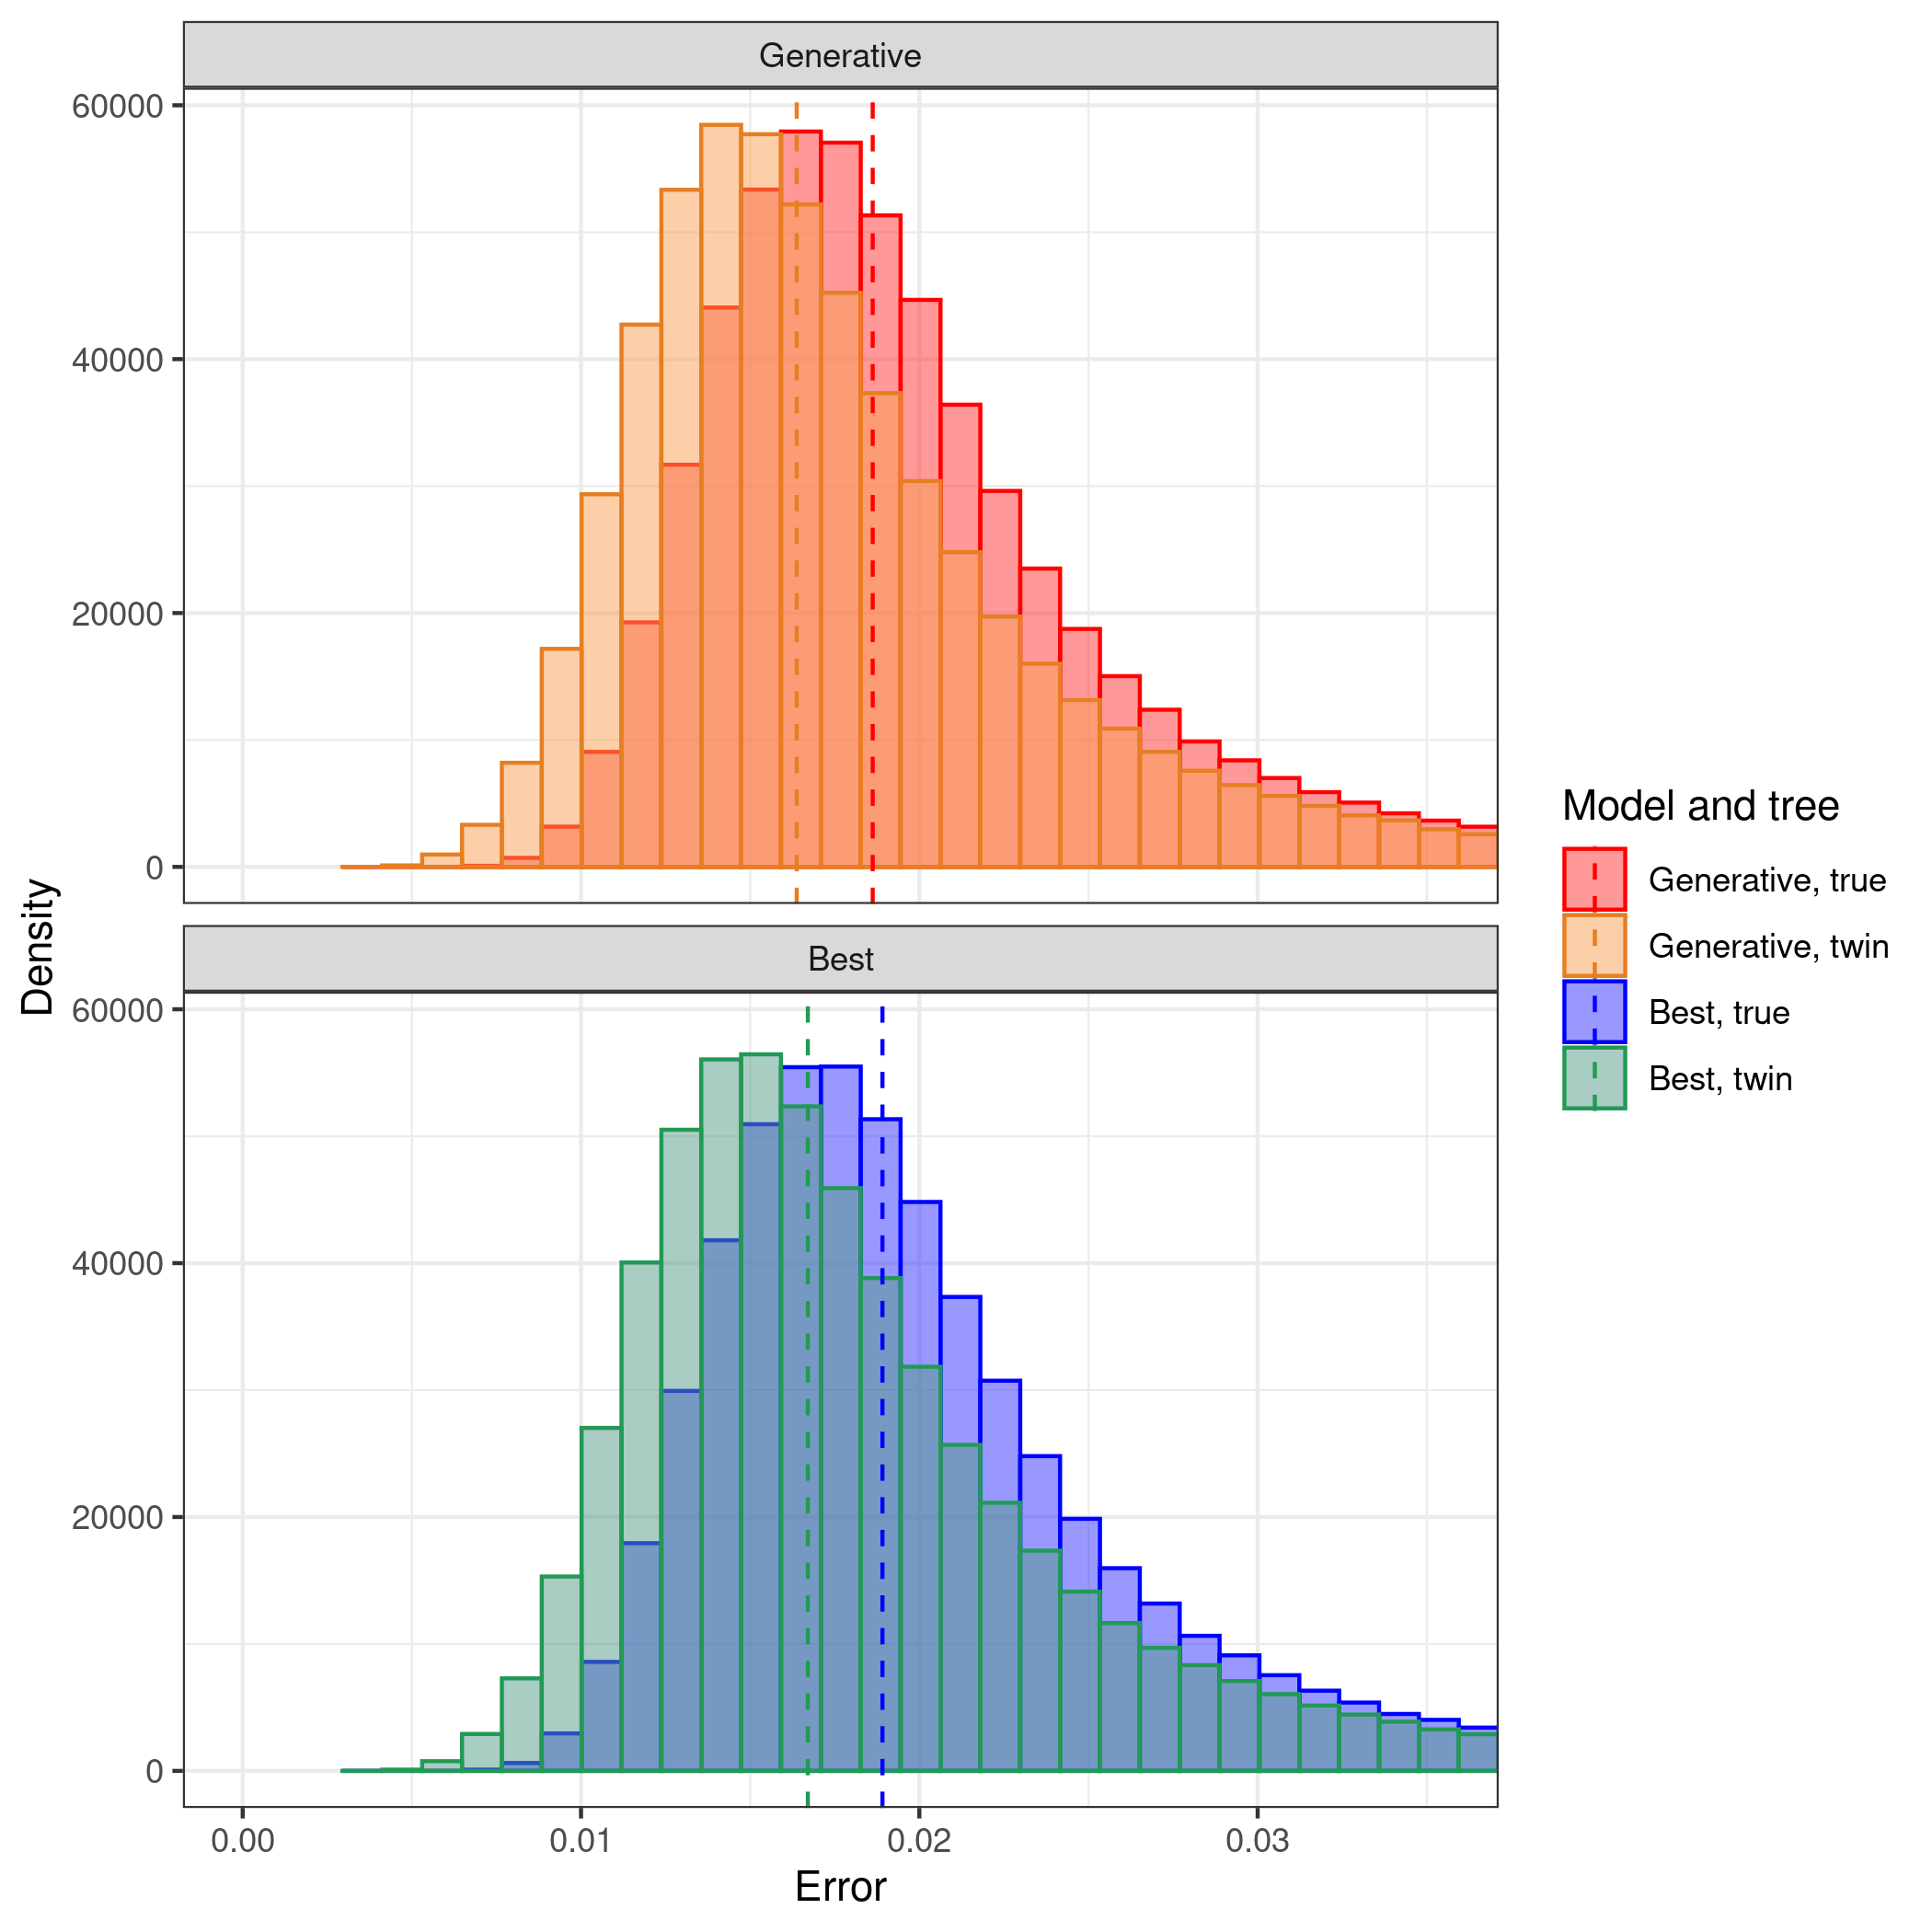
\includegraphics[width=0.98\textwidth]{pirouette_example_41/errors.png}
  \caption{Aggregate error distributions for 65 replicates. Here each true tree has 32 taxa. This took 8.0 days (wall clock time) to compute.}
  \label{fig:example_32_taxa}
\end{figure}

\begin{figure}[H]
  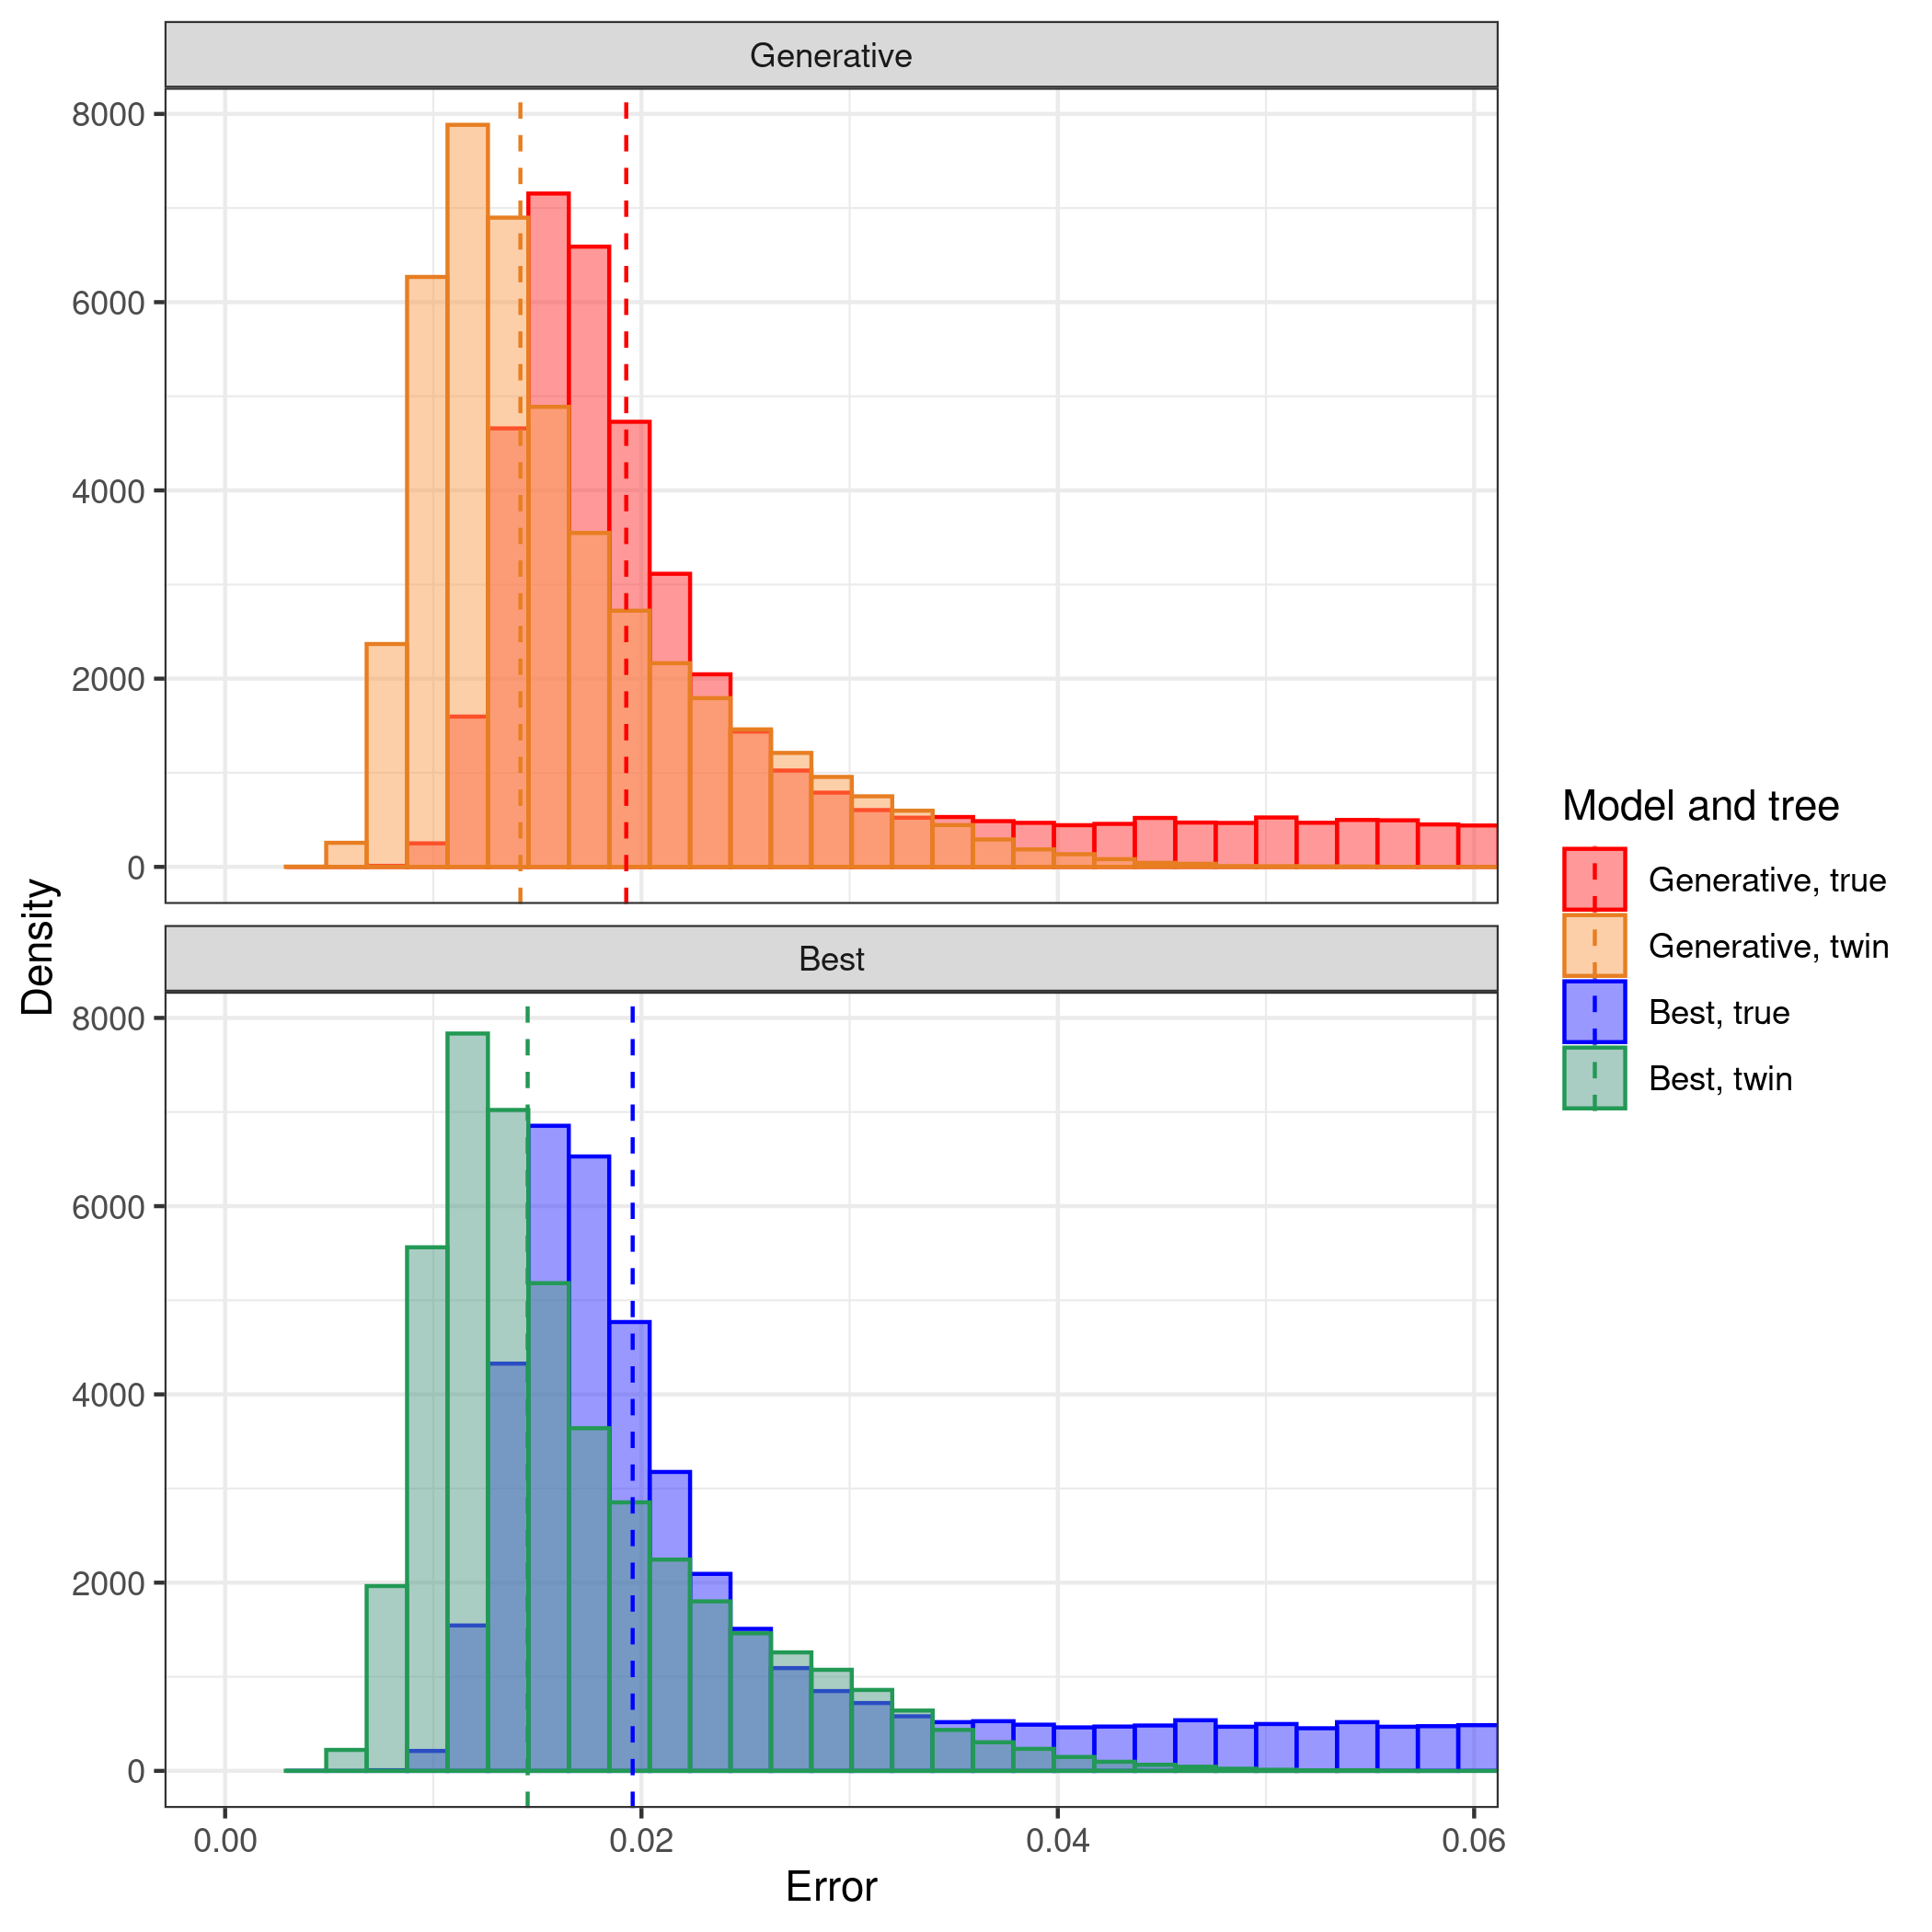
\includegraphics[width=0.98\textwidth]{pirouette_example_42/errors.png}
  \caption{Aggregate error distributions for 5 replicates. Here each true tree has 40 taxa. This took 0.83 days (wall clock time) to compute.}
  \label{fig:example_40_taxa}
\end{figure}

\begin{figure}[H]
  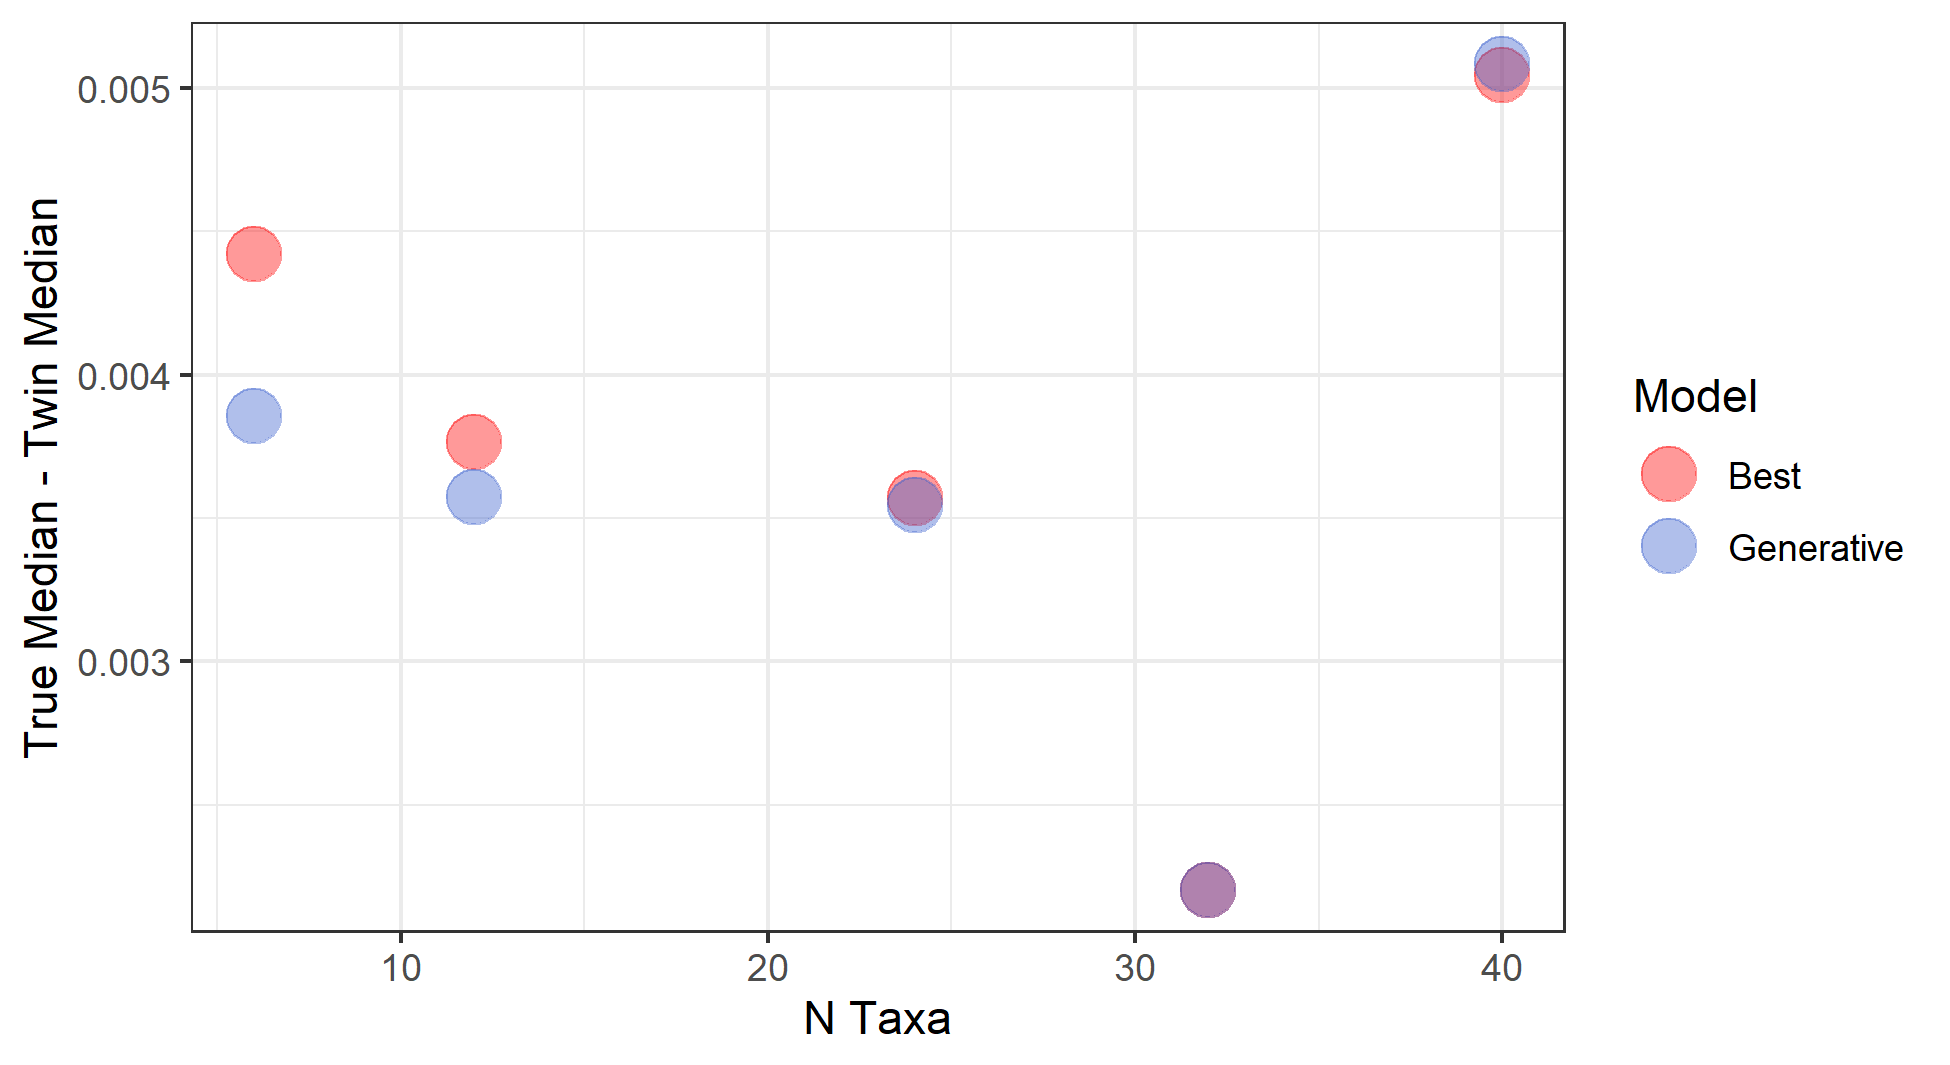
\includegraphics[width=0.98\textwidth]{supplementary_figures/plot_error_vs_n_taxa.png}
  \caption{Difference between median true error and median twin error for different number of taxa.}
  \label{fig:error_vs_ntaxa}
\end{figure}

\new{
  We show in figures \ref{fig:replicate_trees}, \ref{fig:example_12_taxa}, 
  \ref{fig:example_24_taxa}, \ref{fig:example_32_taxa} and 
  \ref{fig:example_40_taxa} what are the errors obtained when starting from 
  phylogenies with, respectively, 6, 12, 24, 32 and 40 taxa.
  Again we can see 
  that in each case errors tend to be greater in the true distribution than 
  in the twin distribution, similar to the result of subsection \ref{subsec:distribution}.
  Collecting all the data together we can see that errors tend to decrease as the number of taxa in the considered phylogenies increase (see Fig. \ref{fig:error_vs_ntaxa}). The data point for $40$ taxa not following the trend could be due to the limited amount of simulated trees taken in consideration due to time constraints.
}

The code to reproduce these figures can be found at  
\begin{sloppypar}
  \url{https://github.com/richelbilderbeek/pirouette_example_28} (6 taxa, main example),
  \url{https://github.com/richelbilderbeek/pirouette_example_32} (12 taxa),
  \url{https://github.com/richelbilderbeek/pirouette_example_33} (24 taxa),
  \url{https://github.com/richelbilderbeek/pirouette_example_41} (32 taxa),
  \url{https://github.com/richelbilderbeek/pirouette_example_42} (40 taxa). 
\end{sloppypar}

\newpage

%%%%%%%%%%%%%%%%%%%%%%%%%%%%%%%%%%%%%%%%%%%%%%%%%%%%%%%%%%%%%%%%%%%%%%%%%%%%%%%%
\subsection{The effect of DNA sequence length}
\label{subsec:n_nucleotides}
%%%%%%%%%%%%%%%%%%%%%%%%%%%%%%%%%%%%%%%%%%%%%%%%%%%%%%%%%%%%%%%%%%%%%%%%%%%%%%%%

The main example uses a DNA alignment length of 1000 nucleotides.
Here, we show the same results as the main example,
except for a varying DNA alignment sequence length.

\begin{figure}[H]
  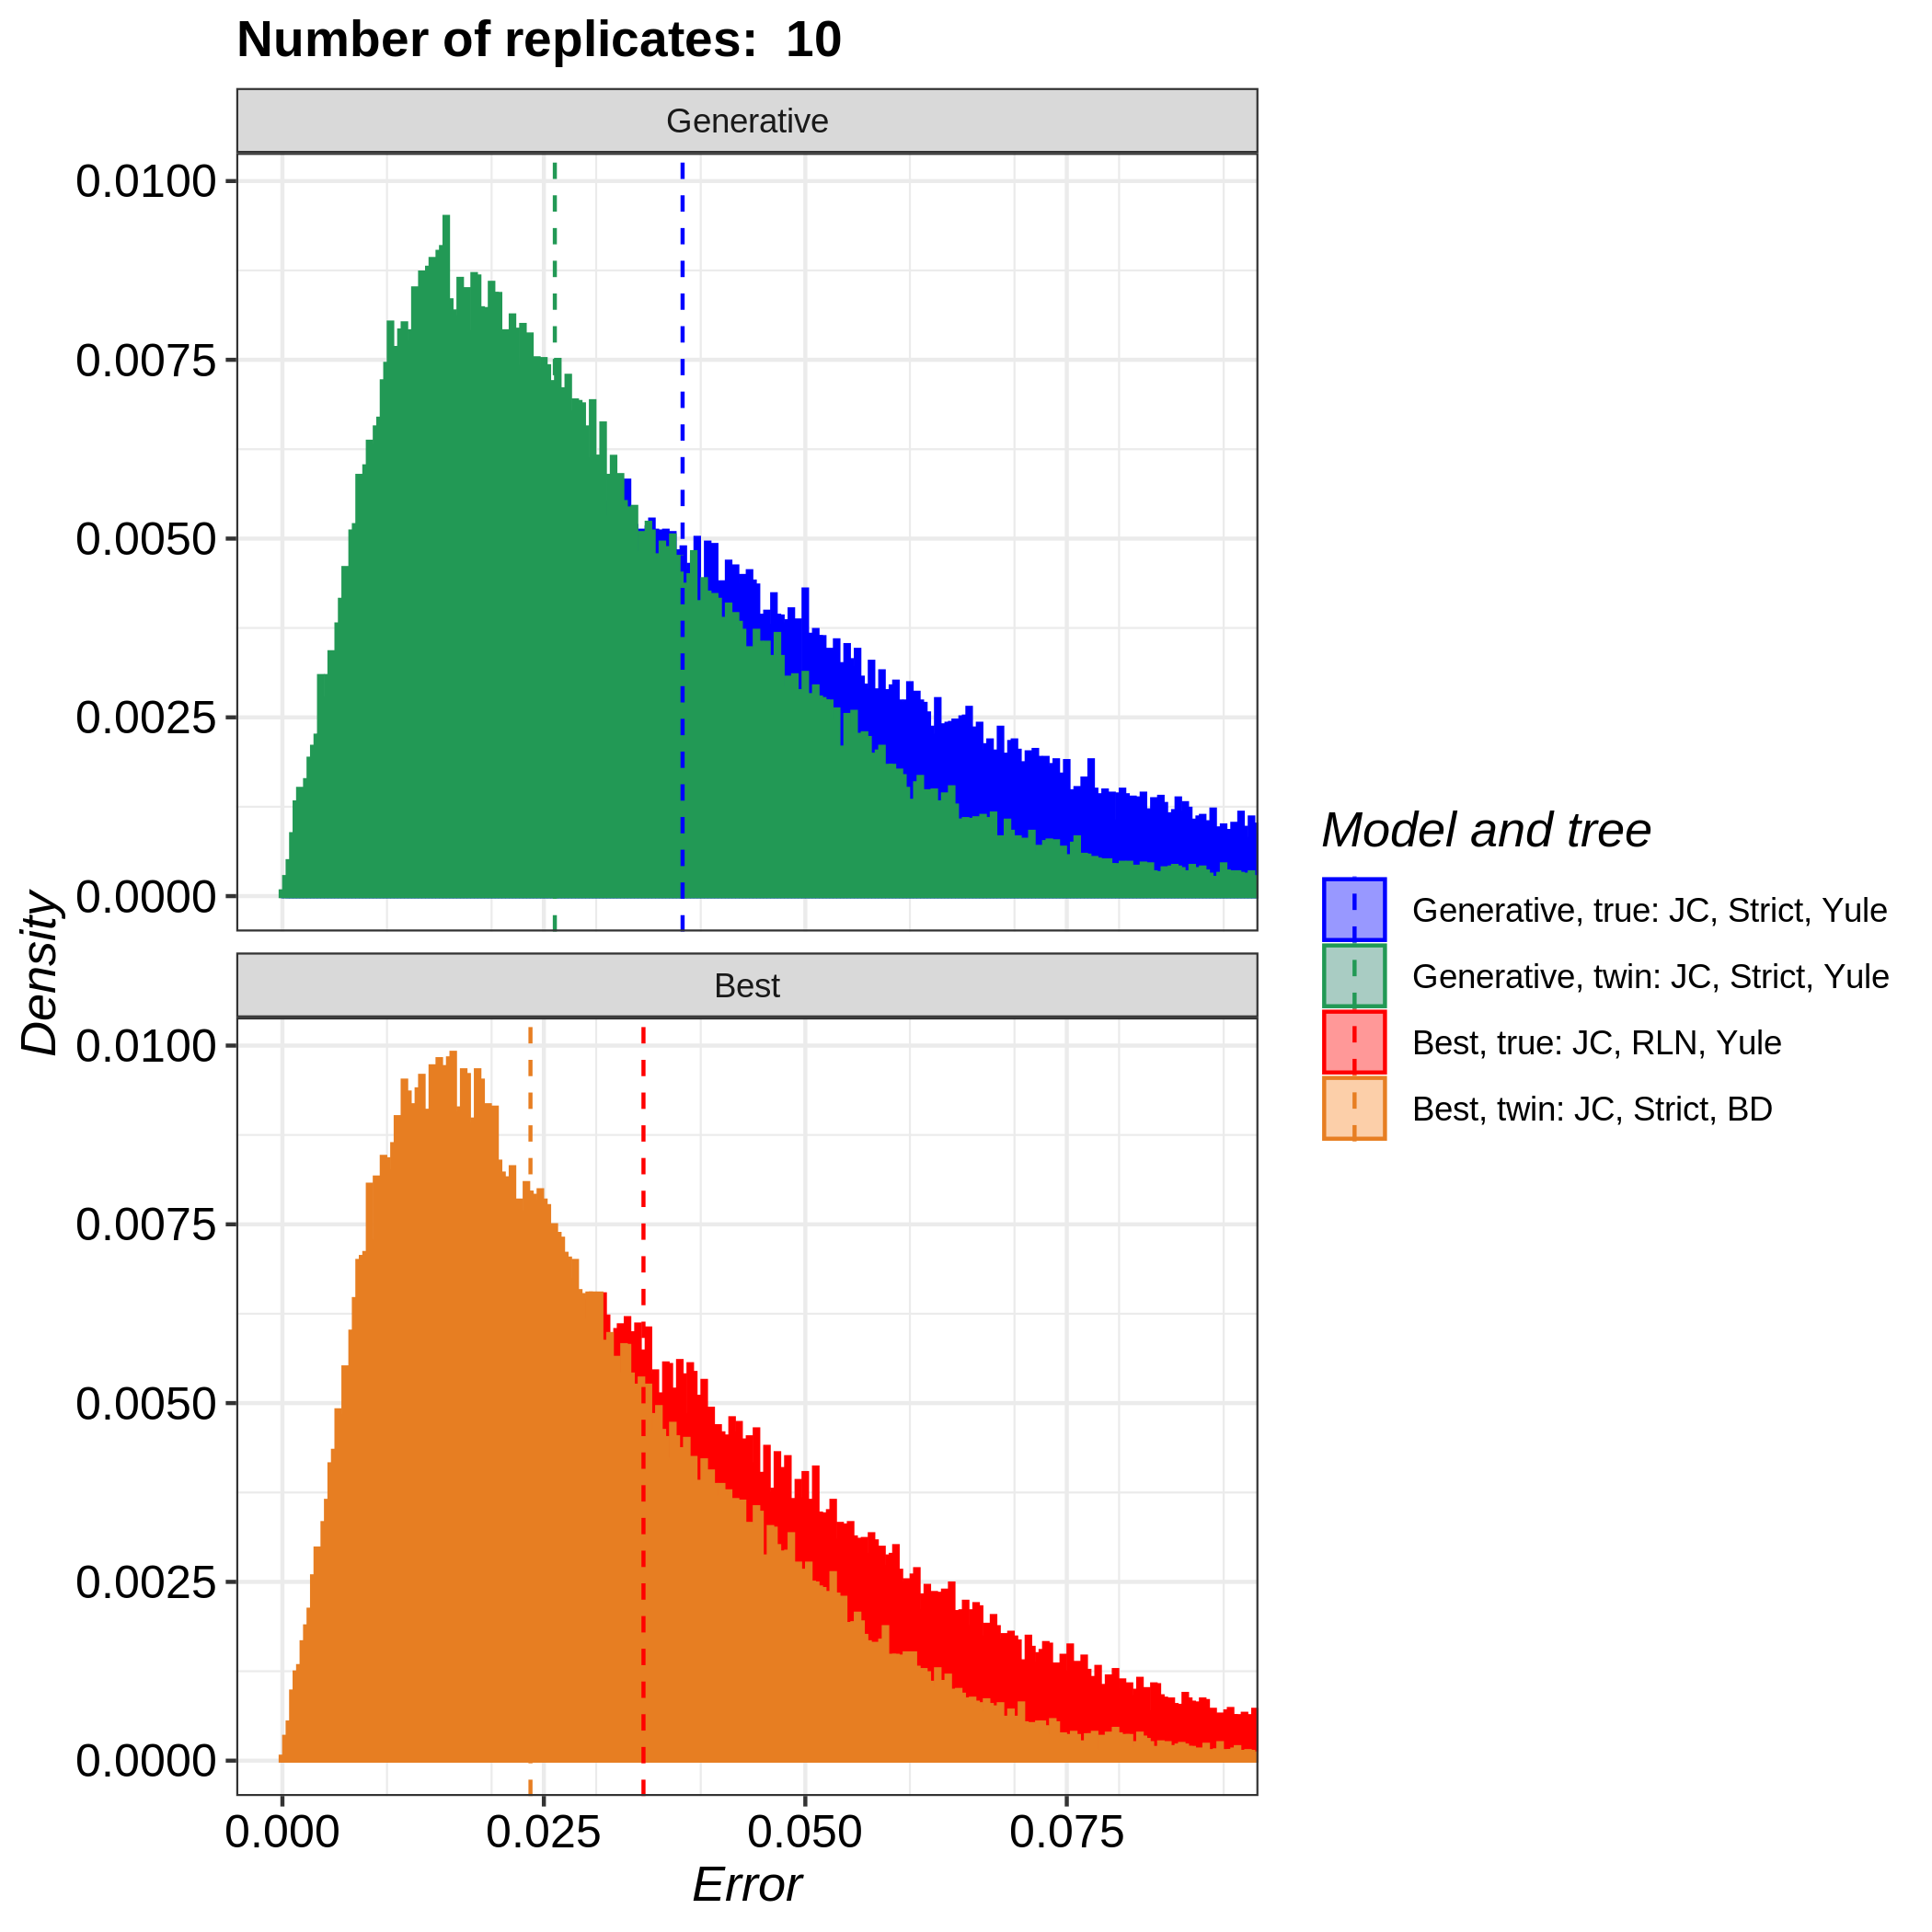
\includegraphics[width=0.98\textwidth]{pirouette_example_19/errors.png}
  \caption{Aggregate error distributions for 100 replicates. 
    Here each each alignment has a sequence length of 500 nucleotides. 
    This took 2.2 days (wall clock time) to compute.}
  \label{fig:example_500_nucleotides}
\end{figure}

\begin{figure}[H]
  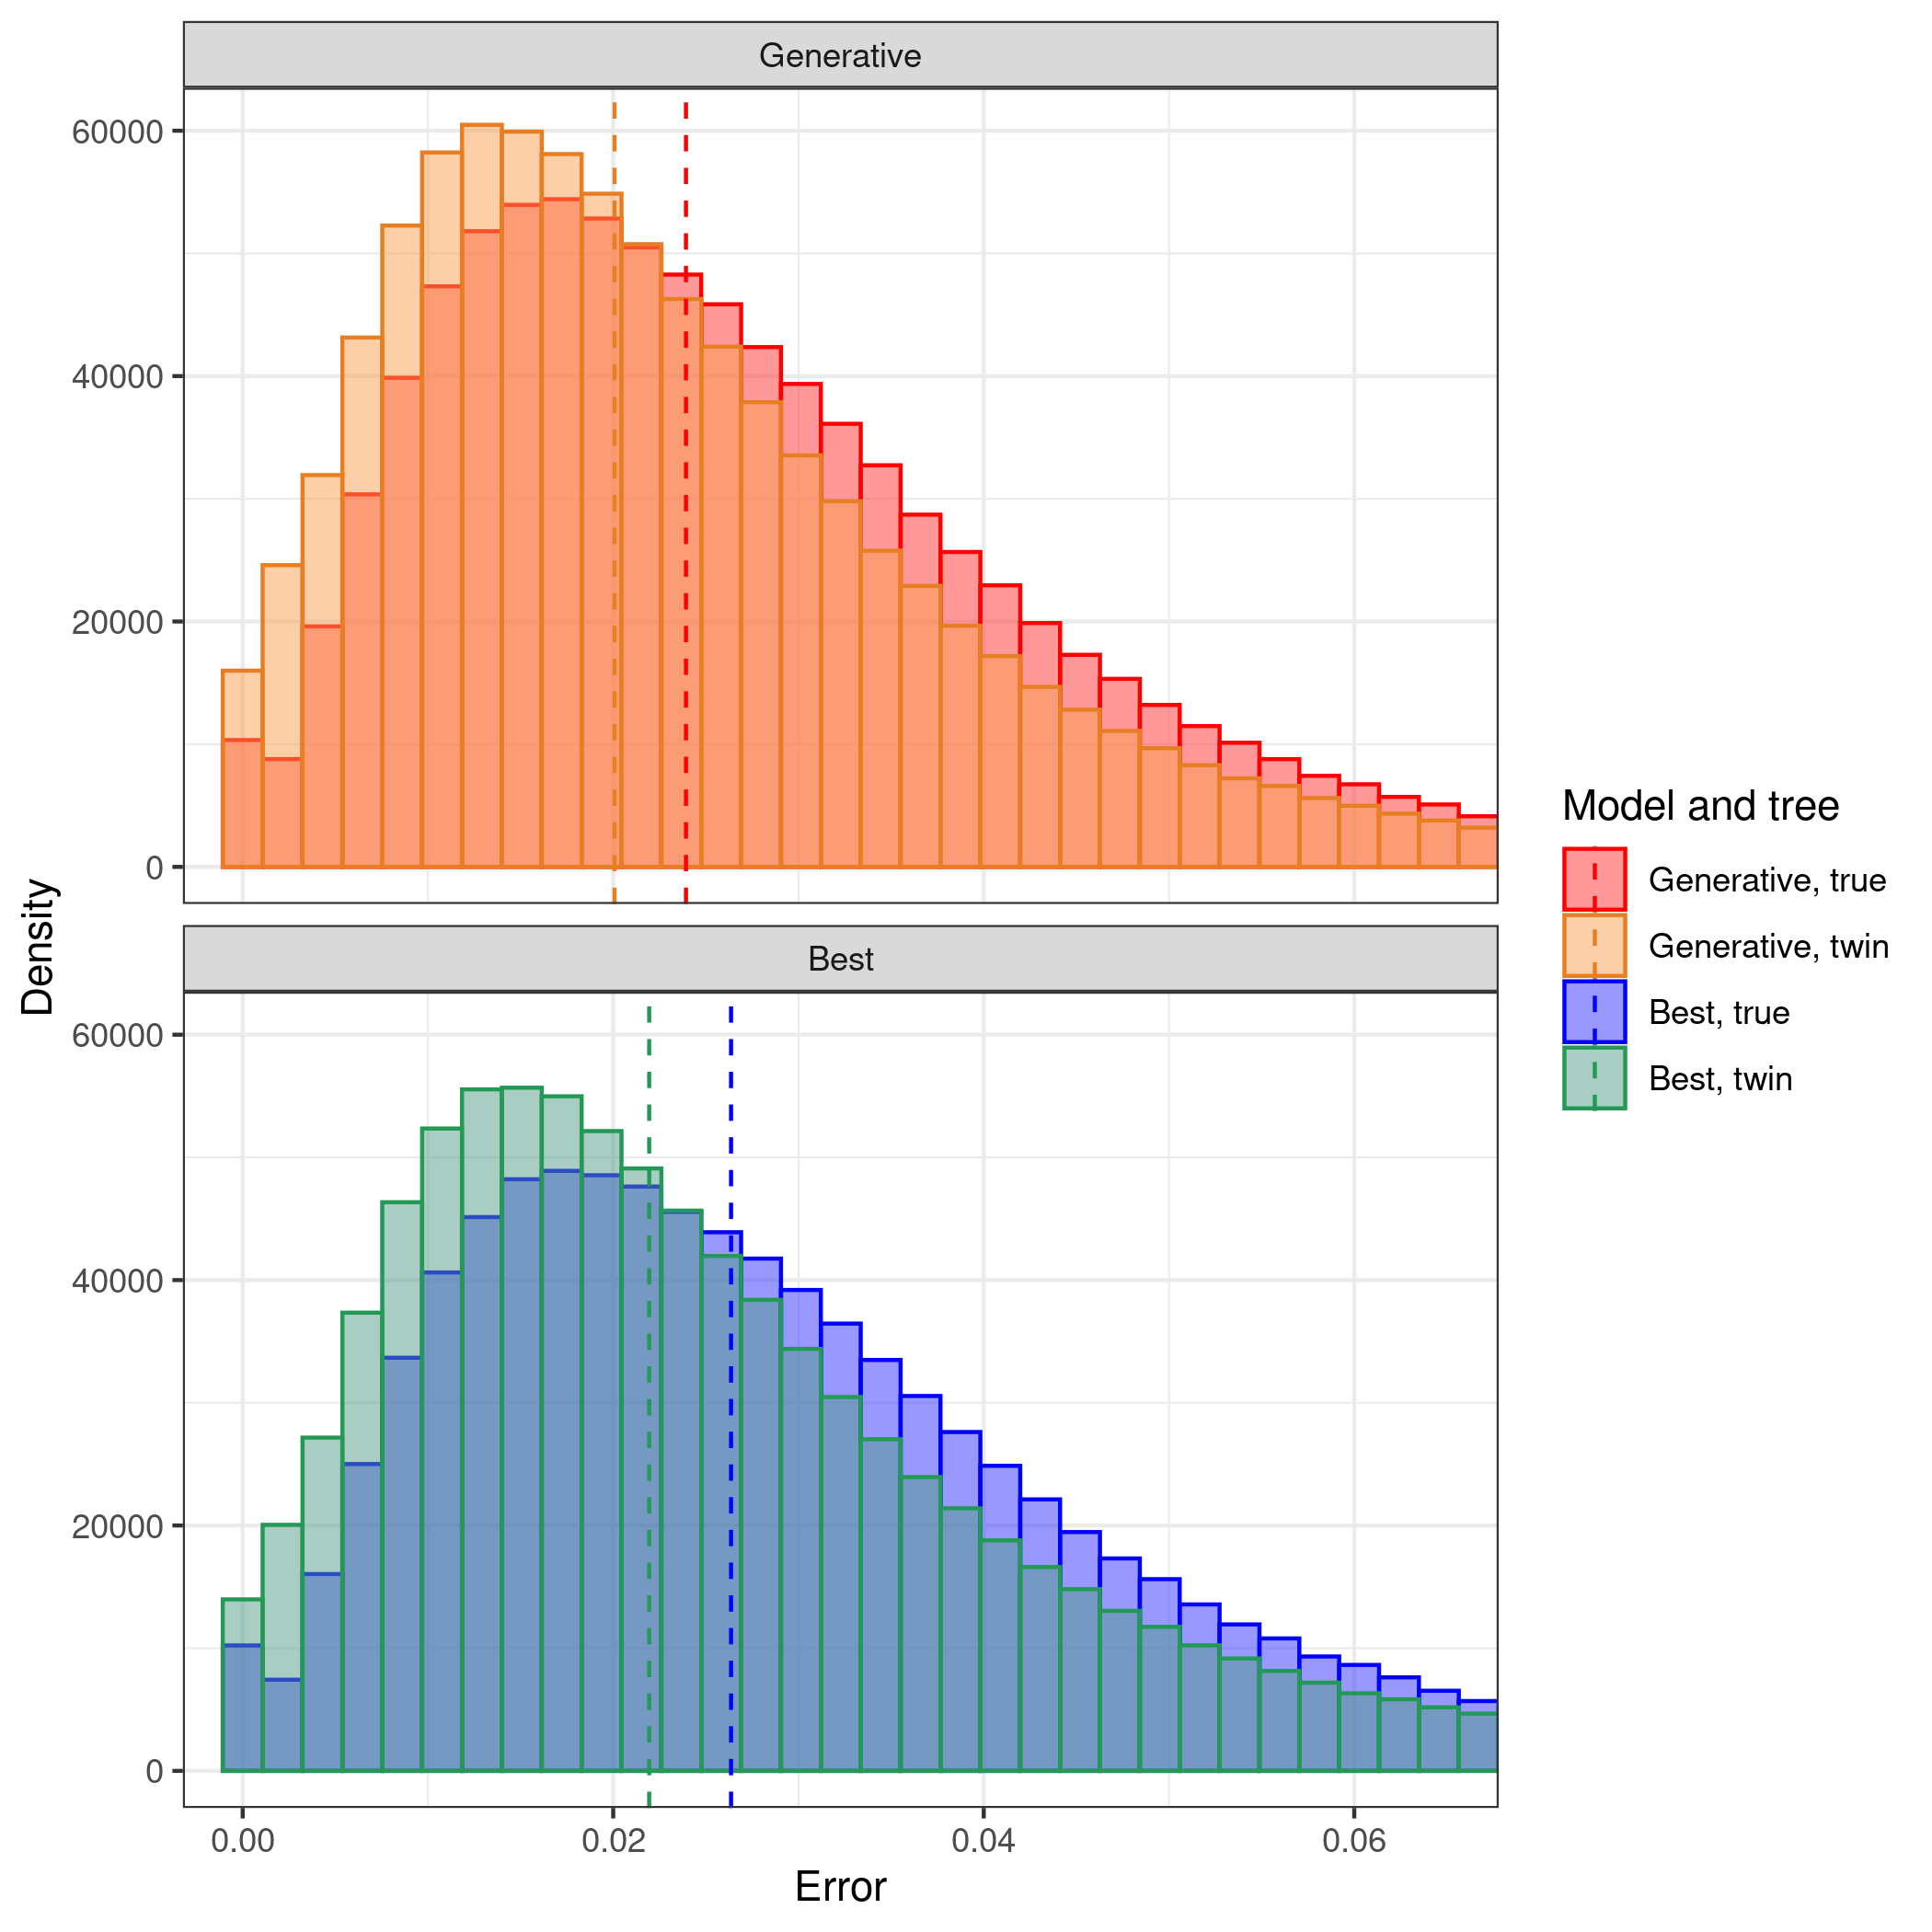
\includegraphics[width=0.98\textwidth]{pirouette_example_28/errors.png}
  \caption{Aggregate error distributions for 100 replicates. 
    Here each each alignment has a sequence length of 1000 nucleotides.
    This is a replicate of Fig. \ref{fig:replicate_trees}. We put it here to facilitate the comparison with the cases with different number of nucleotides.}
  \label{fig:example_1000_nucleotides}
\end{figure}

\begin{figure}[H]
  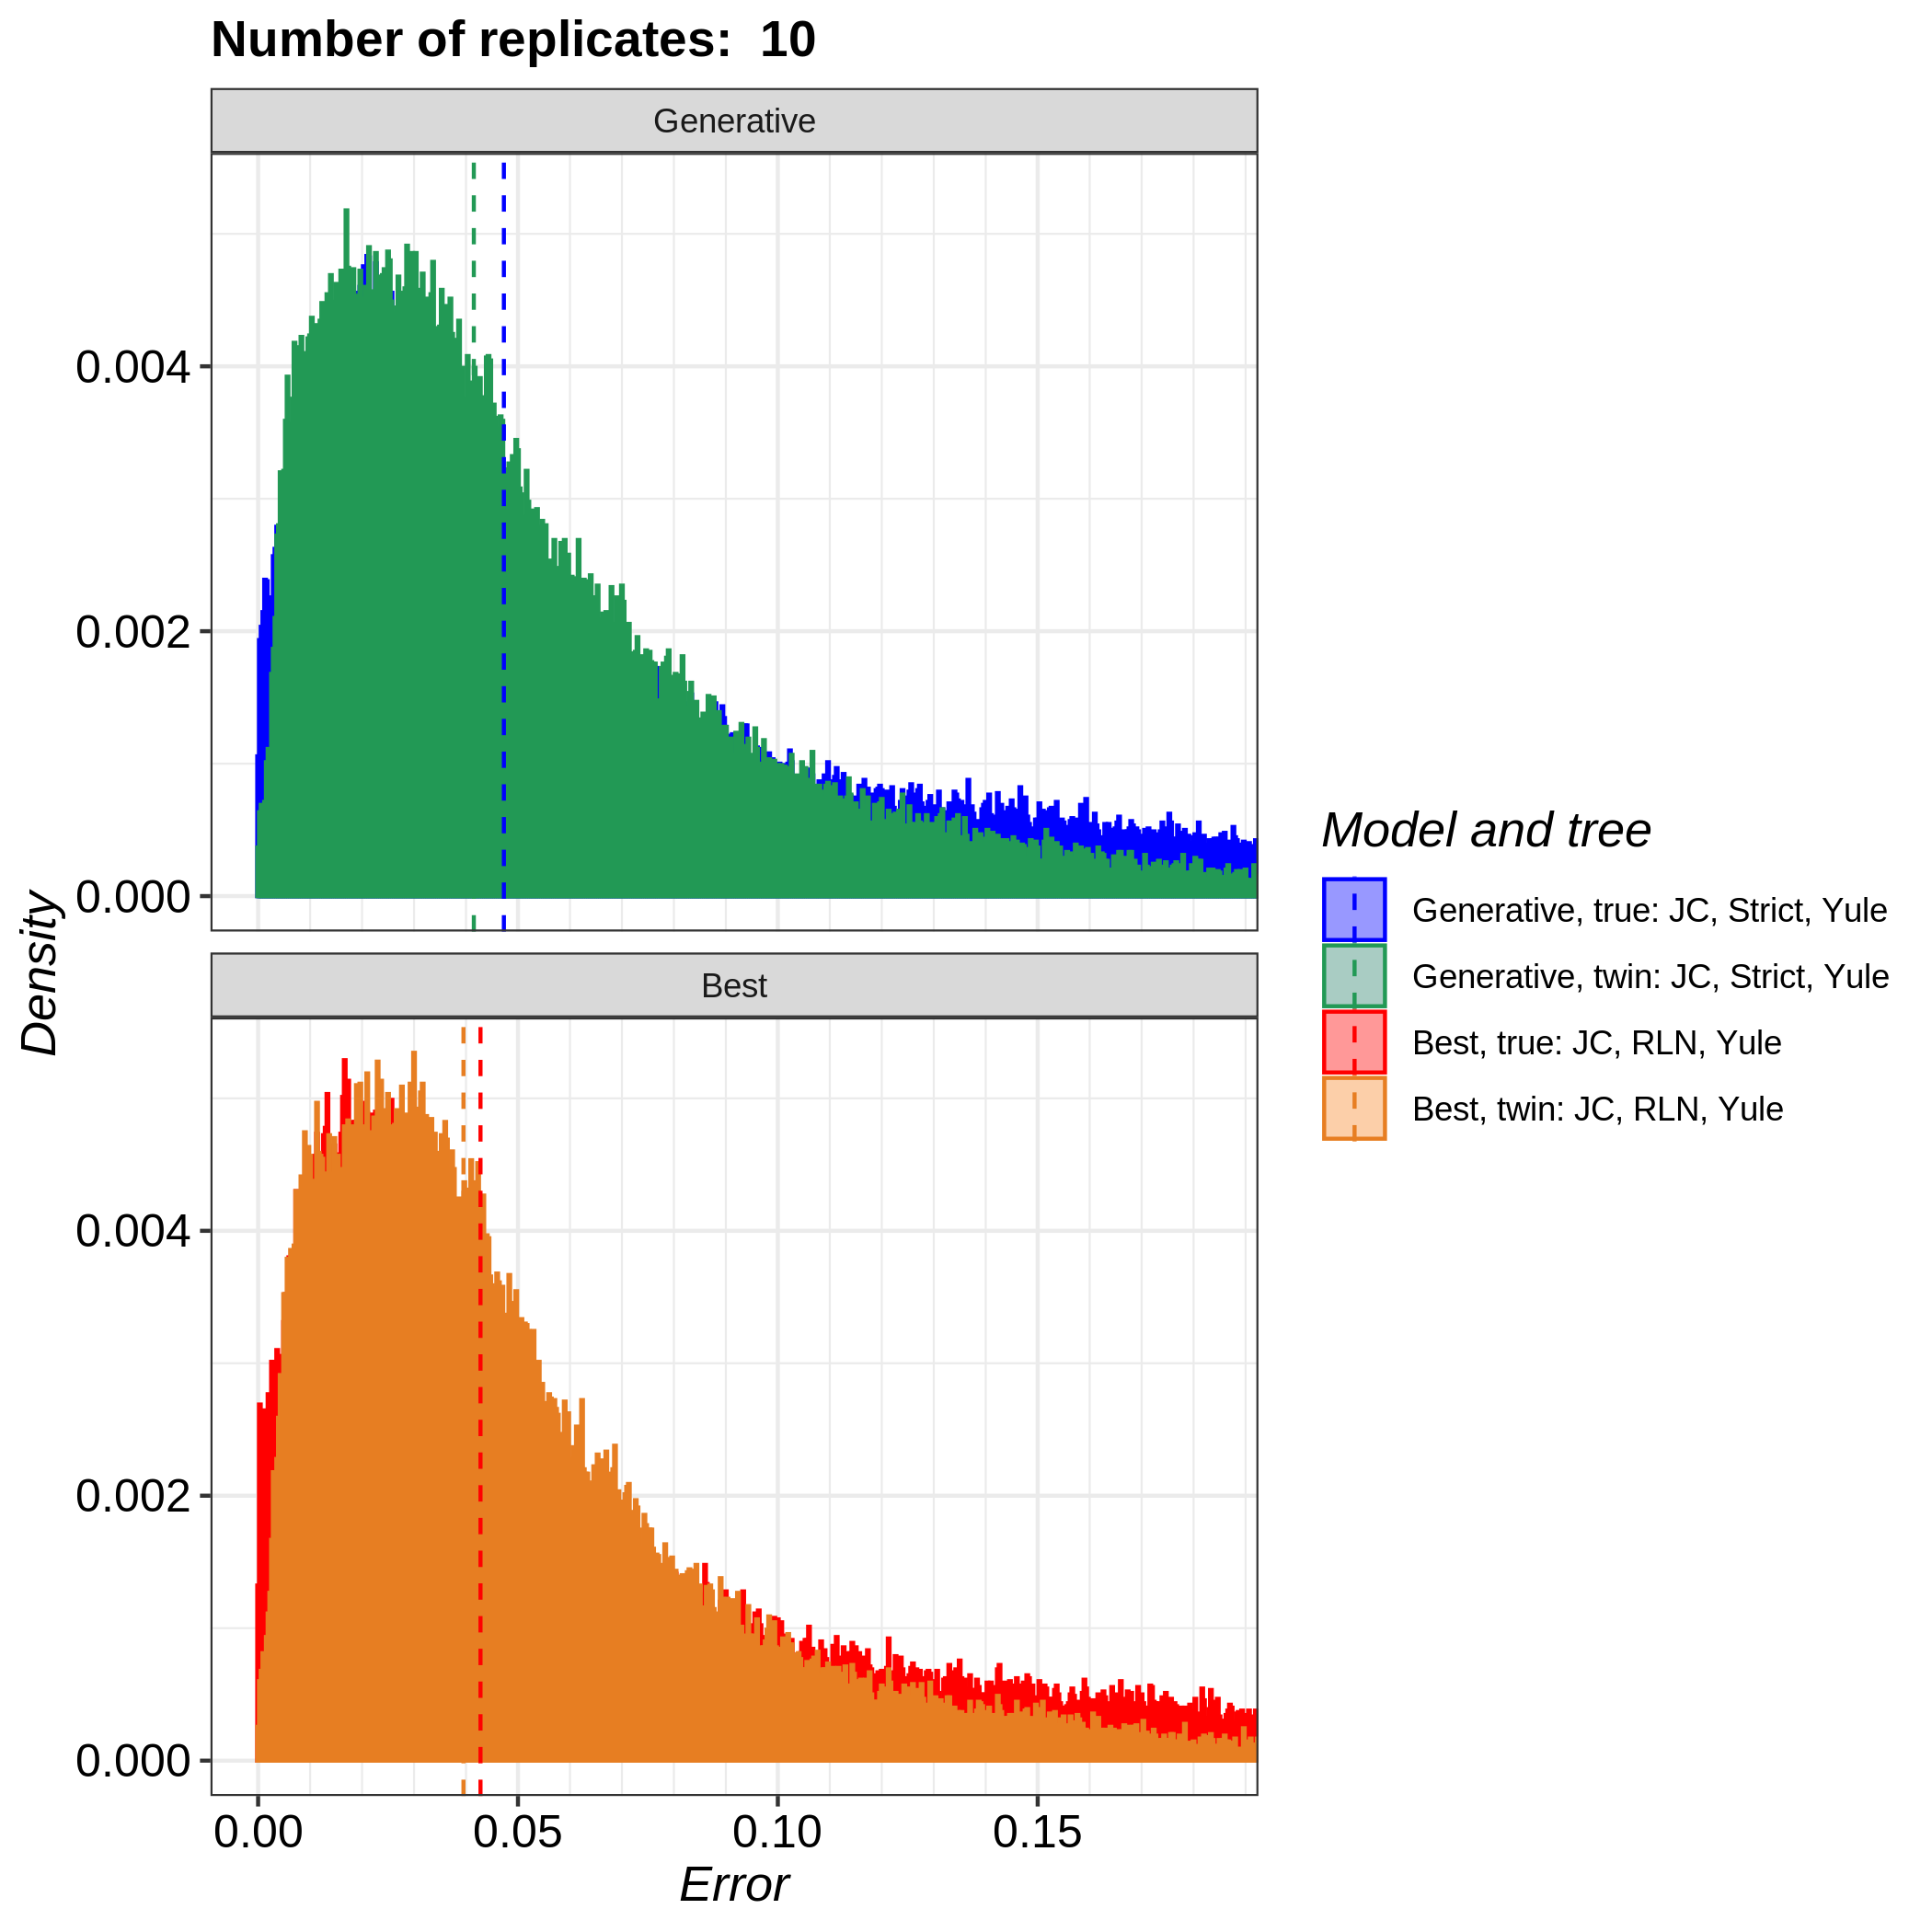
\includegraphics[width=0.98\textwidth]{pirouette_example_34/errors.png}
  \caption{Aggregate error distributions for 100 replicates. 
    Here each each alignment has a sequence length of 2000 nucleotides. 
    This took 4.4 days (wall clock time) to compute.}
  \label{fig:example_2000_nucleotides}
\end{figure}

\begin{figure}[H]
  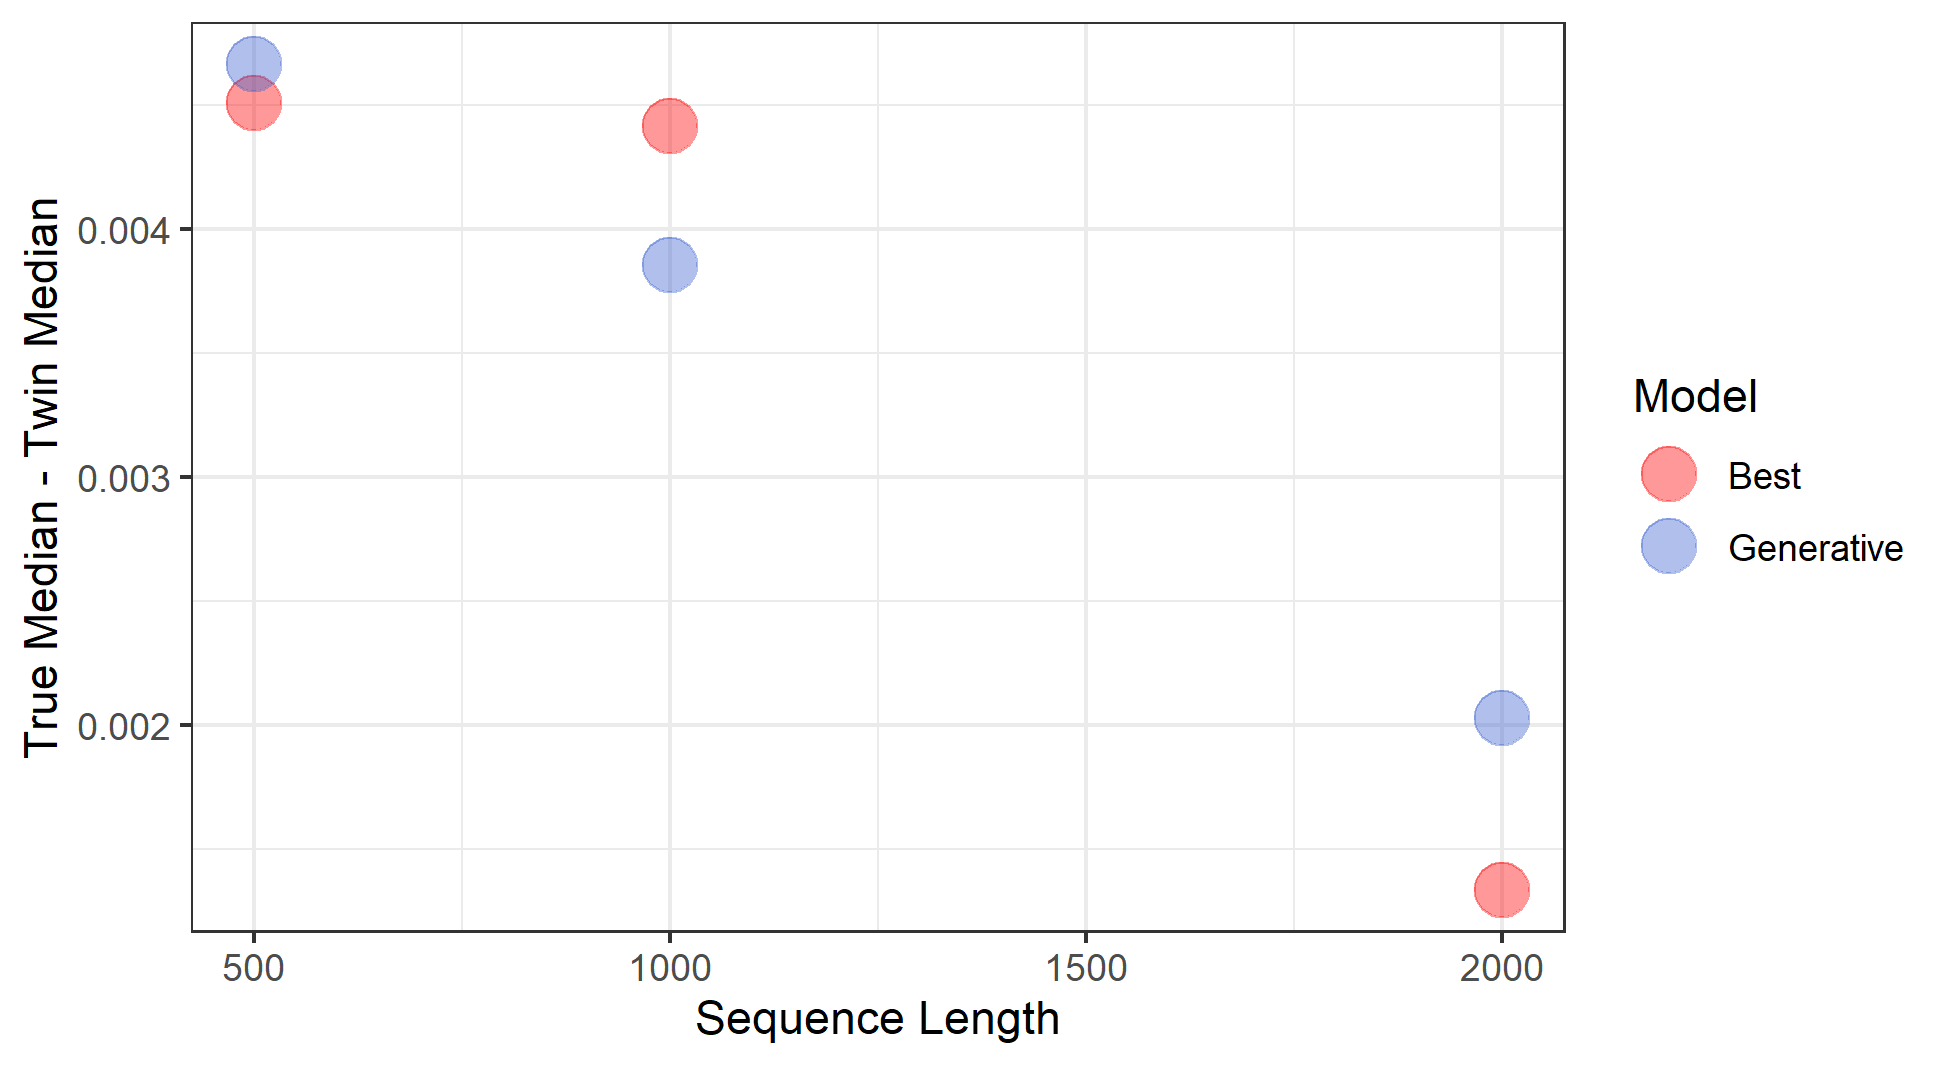
\includegraphics[width=0.98\textwidth]{supplementary_figures/plot_error_vs_sequence_length.png}
  \caption{Difference between median true error and median twin error for different sequence lengths.}
  \label{fig:error_vs_seqlength}
\end{figure}

\new{
  From figures \ref{fig:example_500_nucleotides}, 
  \ref{fig:example_1000_nucleotides} and \ref{fig:example_2000_nucleotides} 
  we can observe that the discrepancy between the true and twin error 
  distributions tends to become smaller as the number of nucleotides increase (see also Fig. \ref{fig:error_vs_seqlength}).
  This occurred for both the generative and best candidate cases.
  This follows the expectation that a prior becomes less important when
  more information becomes available.
}

The code to reproduce these figures can be found at  
\begin{sloppypar}
  \url{https://github.com/richelbilderbeek/pirouette_example_19} (500 nucleotides),
  \url{https://github.com/richelbilderbeek/pirouette_example_28} (1000 nucleotides, main example),
  and \url{https://github.com/richelbilderbeek/pirouette_example_34} (2000 nucleotides).
\end{sloppypar}

\newpage

%%%%%%%%%%%%%%%%%%%%%%%%%%%%%%%%%%%%%%%%%%%%%%%%%%%%%%%%%%%%%%%%%%%%%%%%%%%%%%%%
\subsection{The effect of assuming a Yule tree prior on a Yule tree}
\label{subsec:simplest_correct_parameterization}
%%%%%%%%%%%%%%%%%%%%%%%%%%%%%%%%%%%%%%%%%%%%%%%%%%%%%%%%%%%%%%%%%%%%%%%%%%%%%%%%

The main example uses a tree generated by a non-standard tree model.
Here, we show the same results, with the only difference that
the tree used is generated by simplest tree model (the Yule model),
which we also assume as the (correct) tree prior.

\begin{figure}[H]
  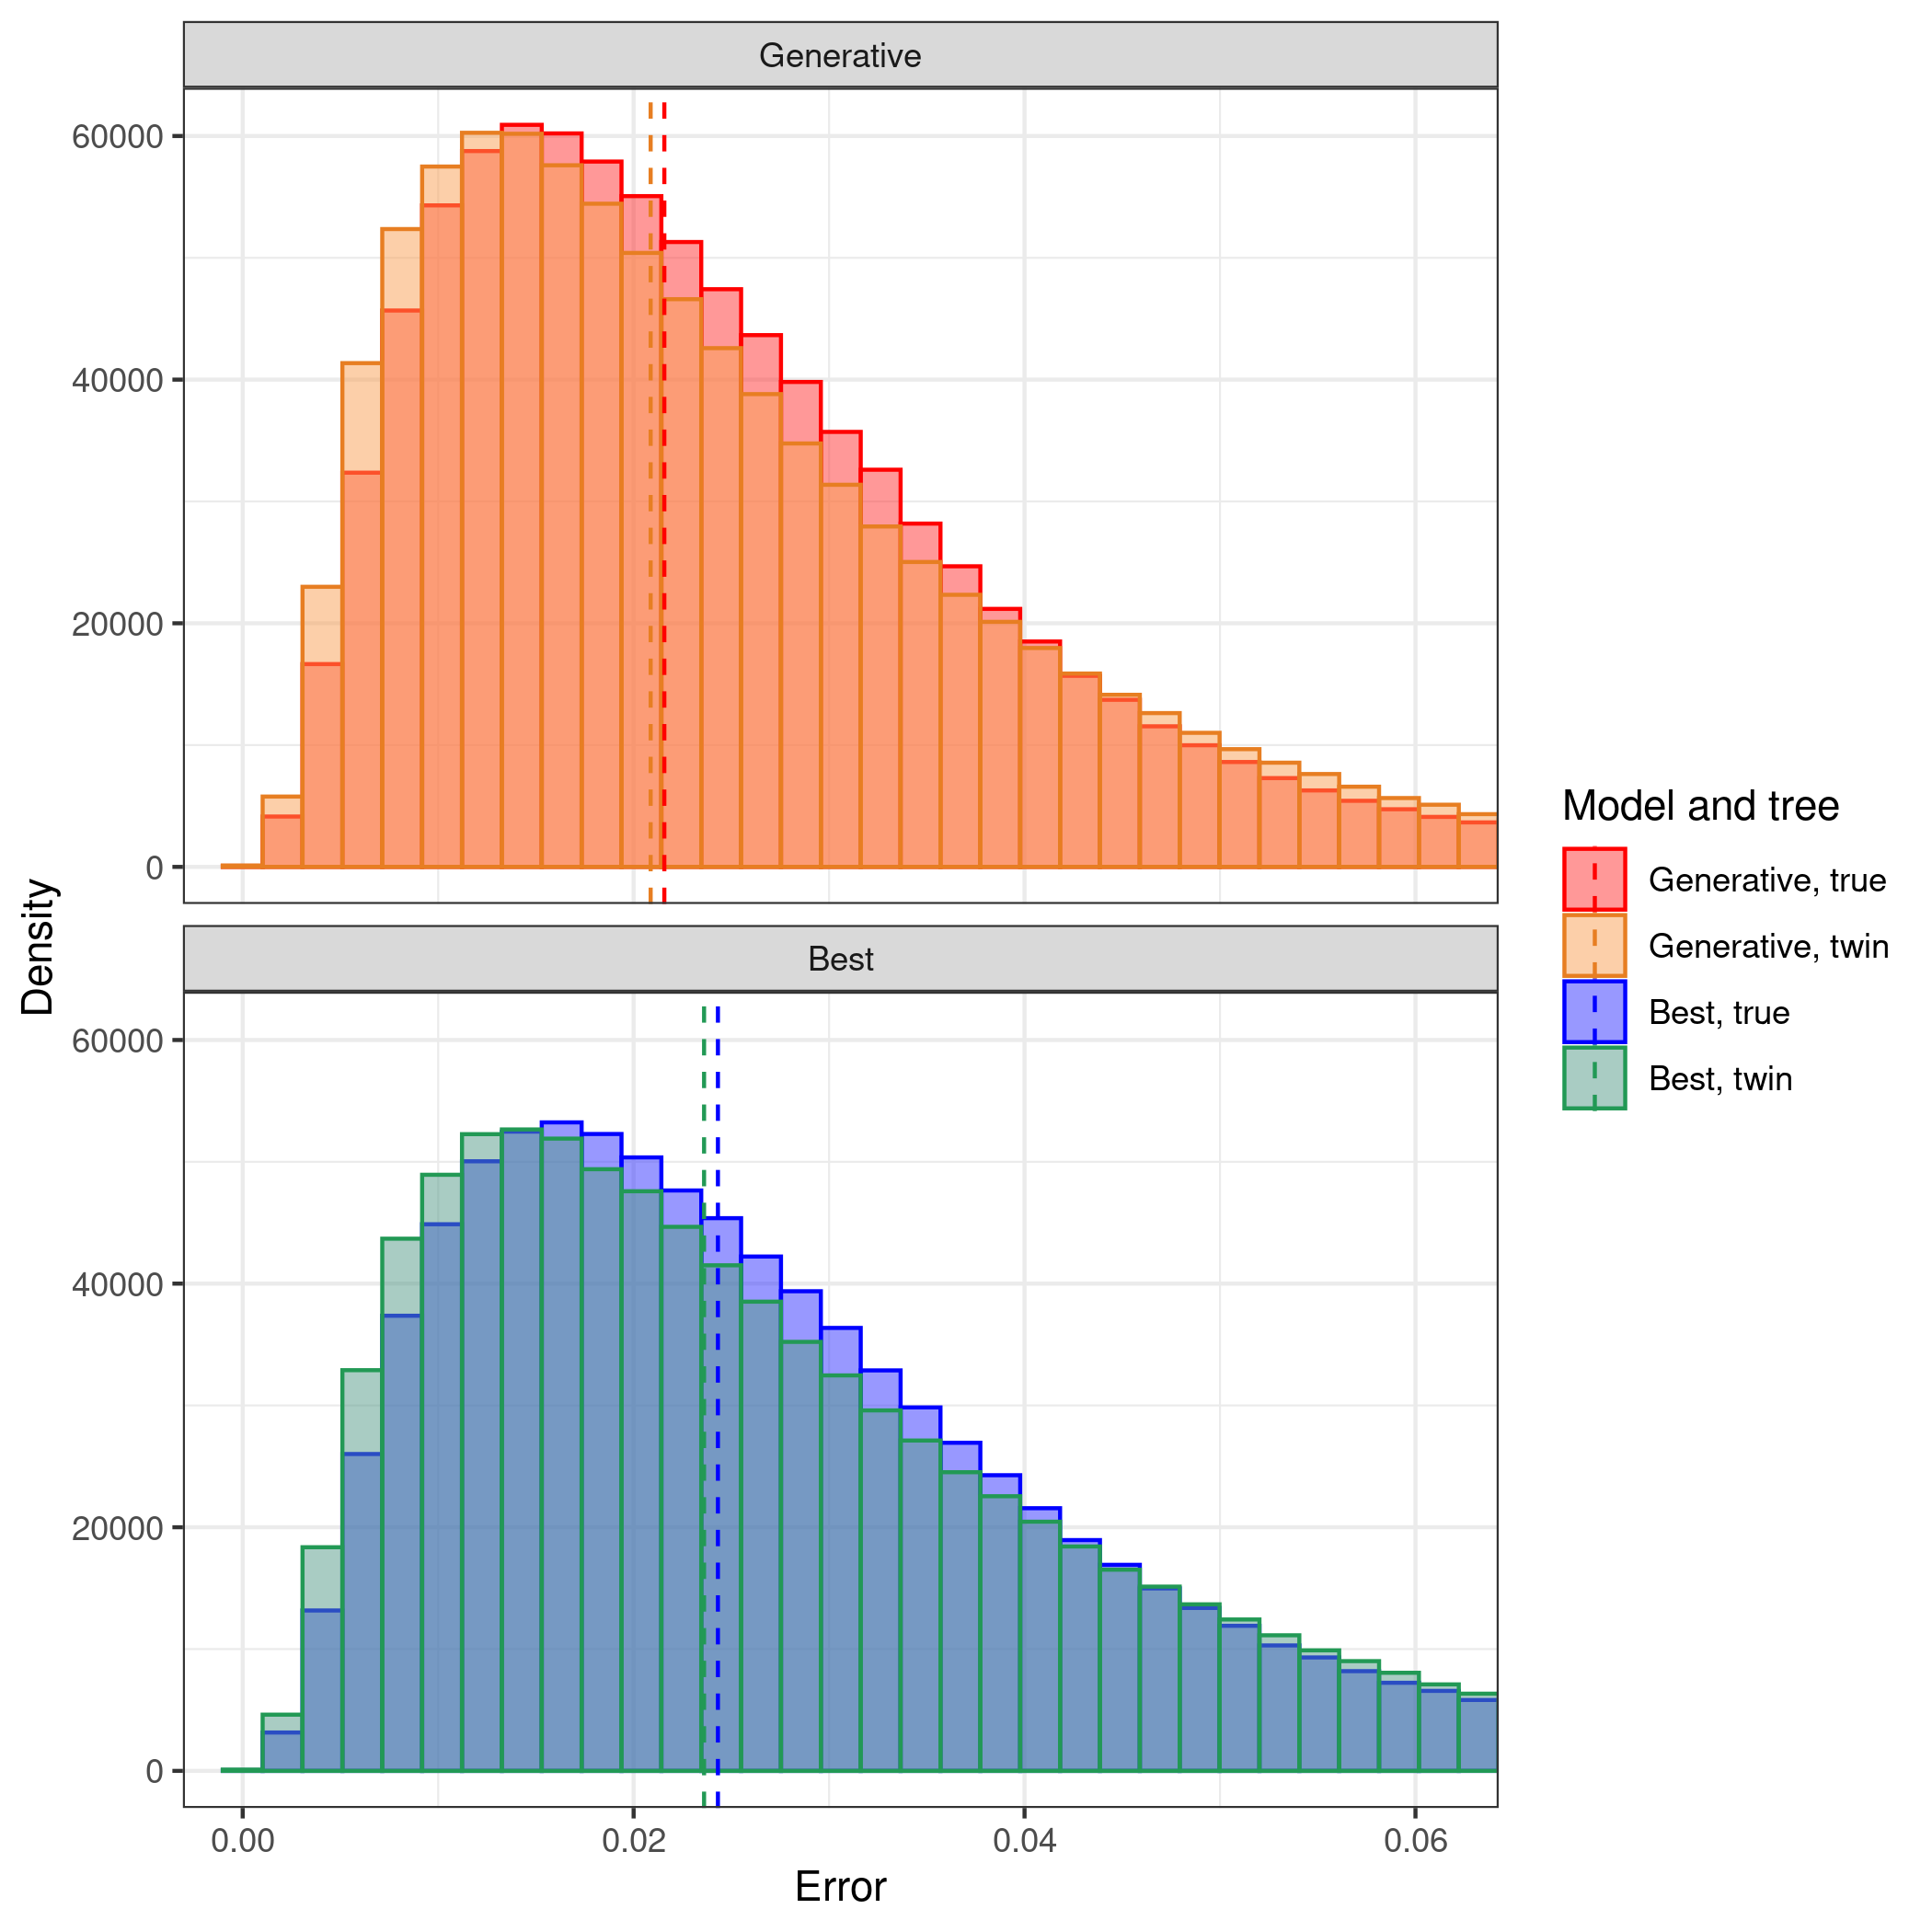
\includegraphics[width=0.98\textwidth]{pirouette_example_22/errors.png}
  \caption{Aggregate error distributions for 100 replicates. 
    Here each true tree is generated by a Yule process. 
    For the inference we used a Yule tree prior. 
    This took 2.9 days (wall clock time) to compute.}
  \label{fig:example_yule}
\end{figure}

This example shows a parameterization at the correct level for the
simplest case possible.

\new{
  As expected the twin and true distributions in Fig. \ref{fig:example_yule} 
  are extremely similar for both the generative and the best candidate case.
}

The code to reproduce this figure can be found at  
\begin{sloppypar}
  \url{https://github.com/richelbilderbeek/pirouette_example_22}.
\end{sloppypar}

\newpage

%%%%%%%%%%%%%%%%%%%%%%%%%%%%%%%%%%%%%%%%%%%%%%%%%%%%%%%%%%%%%%%%%%%%%%%%%%%%%%%%
\subsection{The effect of assuming a Yule tree prior on a BD tree}
\label{subsec:under_parameterization}
%%%%%%%%%%%%%%%%%%%%%%%%%%%%%%%%%%%%%%%%%%%%%%%%%%%%%%%%%%%%%%%%%%%%%%%%%%%%%%%%

The main example uses a tree generated by a non-standard tree model.
Here, we show the same results, with the difference that
the tree used is generated by a birth-death (BD) tree model,
where we assume it is generated by a Yule (or pure-birth) model.
This example thus shows the effect of underparameterization.

\begin{figure}[H]
  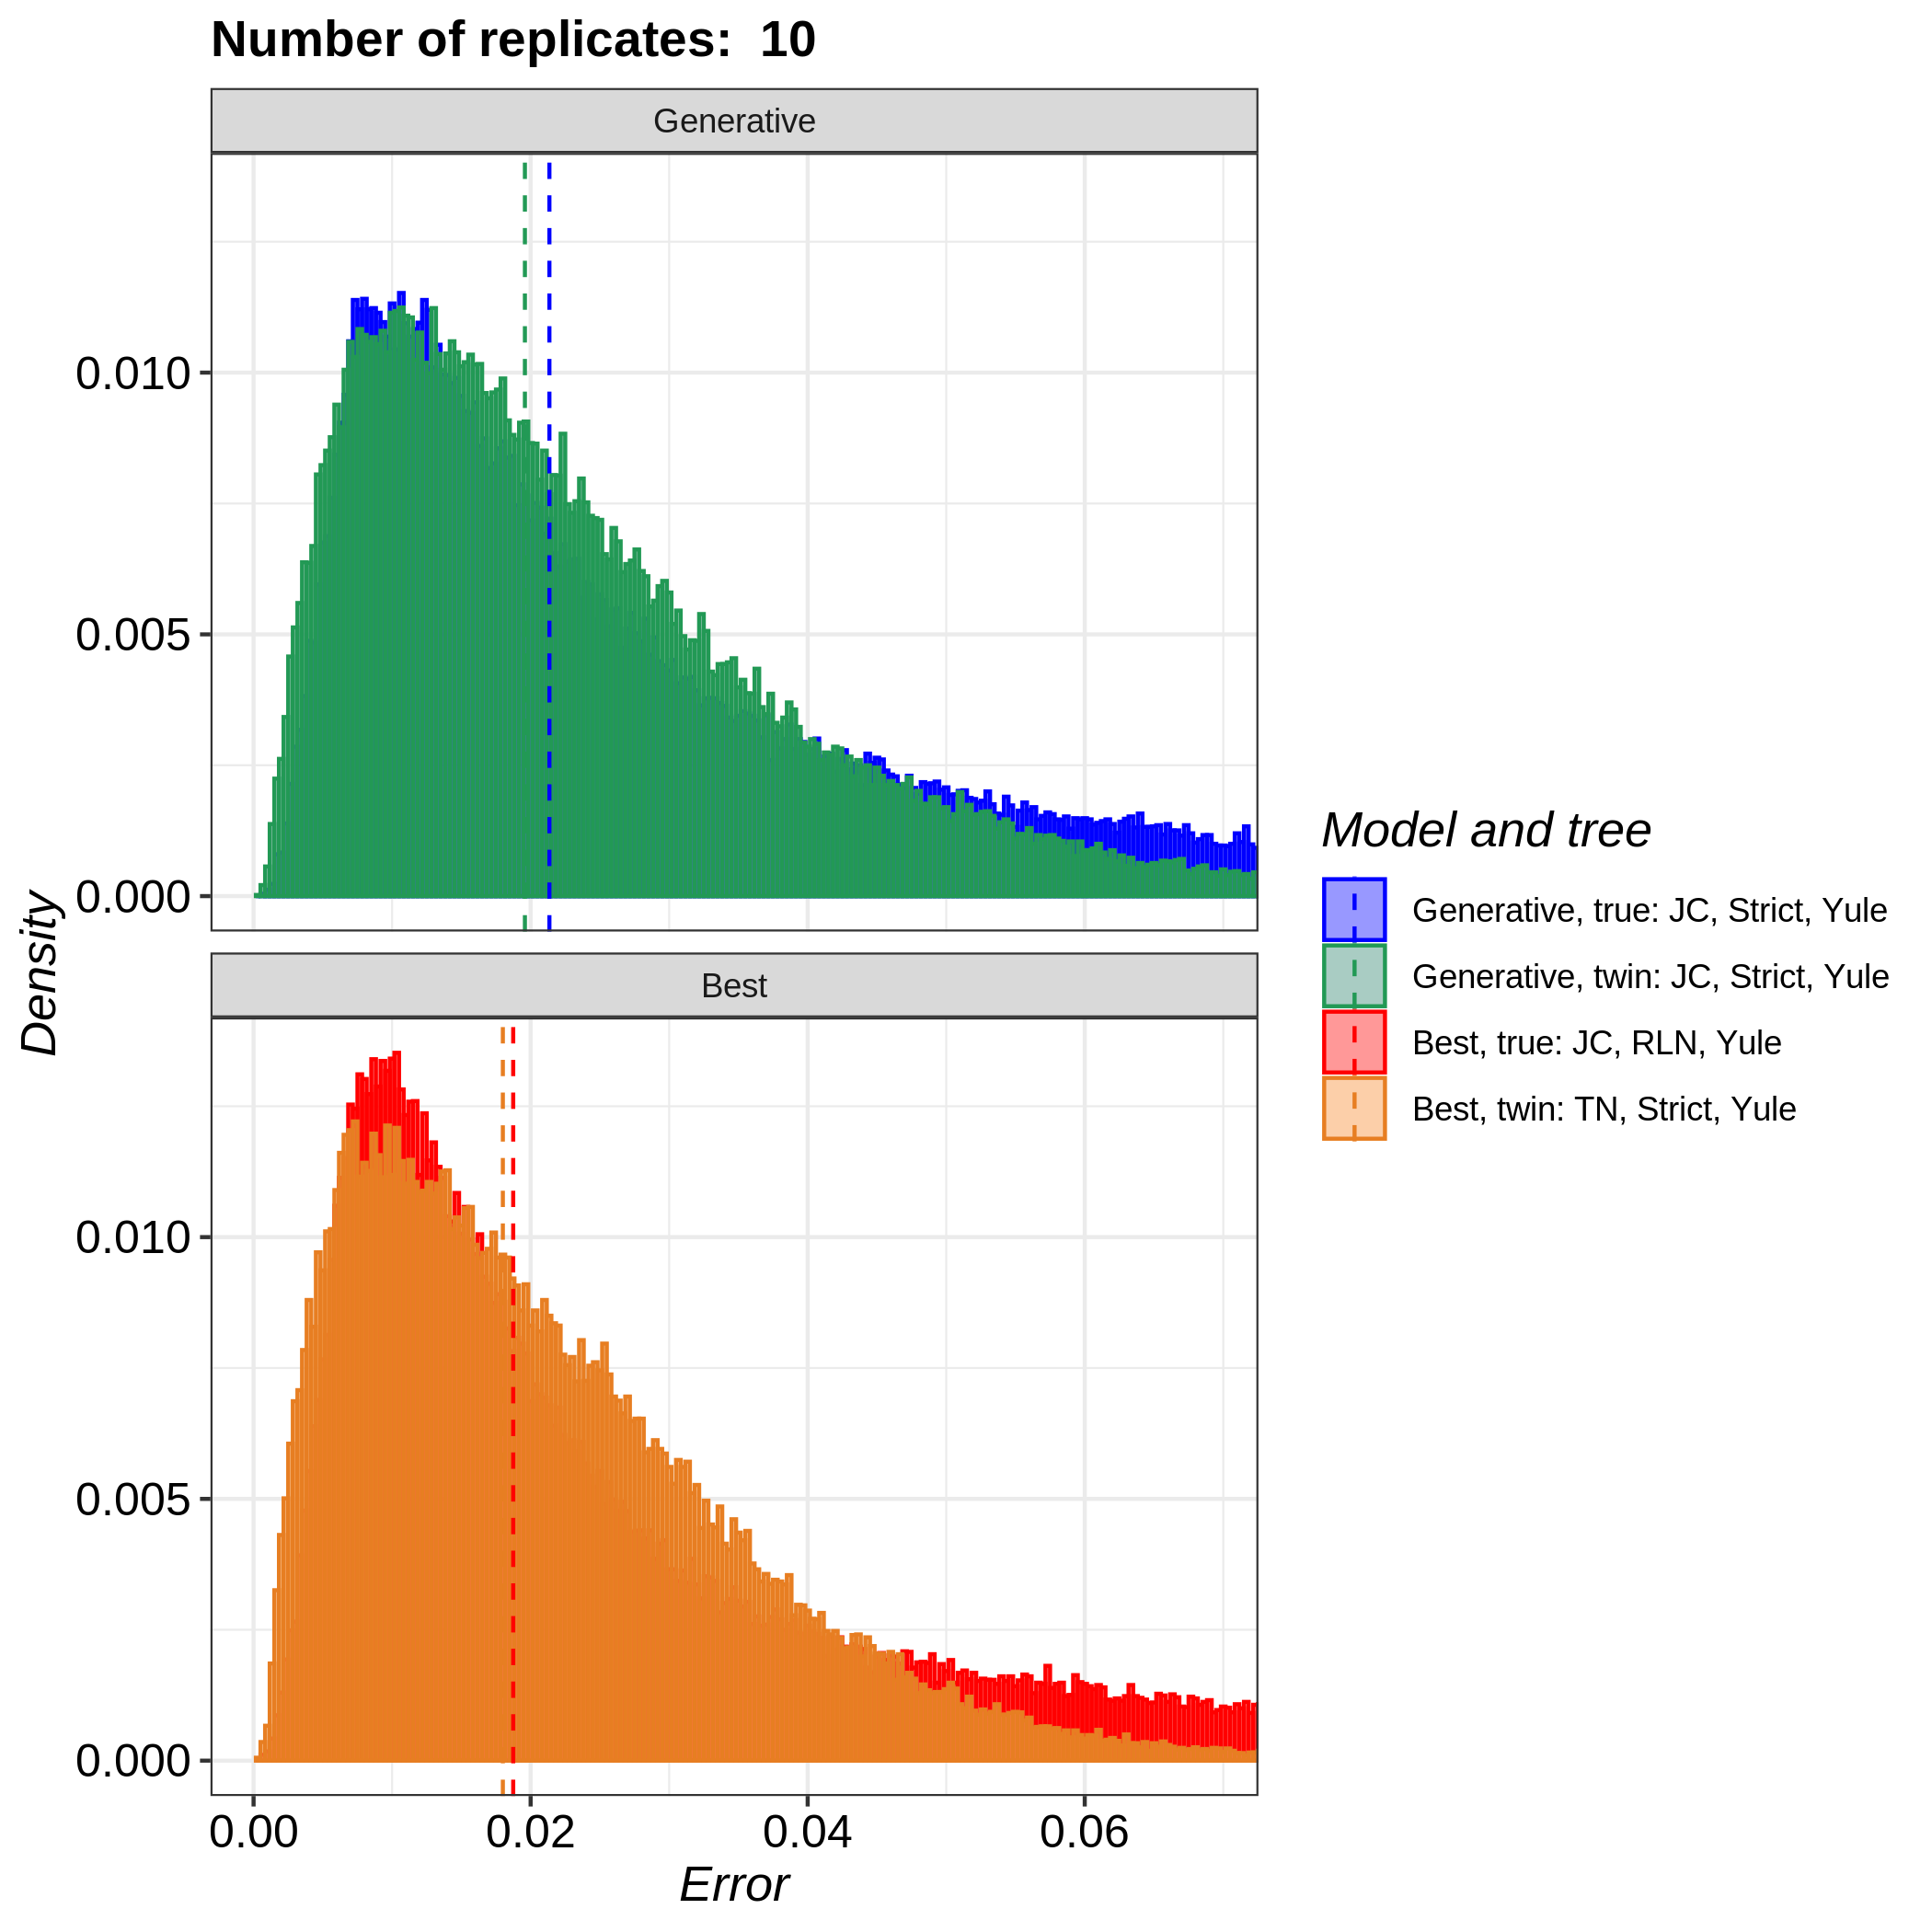
\includegraphics[width=0.98\textwidth]{pirouette_example_26/errors.png}
  \caption{Aggregate error distributions for 100 replicates. 
    Here each true tree is generated by a BD process. 
    For the inference we used instead a Yule tree prior. 
    This took 2.7 days (wall clock time) to compute.}
\end{figure}

\new{
  Because the two models are very similar to each other (the BD model can be 
  turned into a Yule model just by setting the extinction parameter to 
  zero [\cite{nee1994reconstructed}]) the median discrepancy is
  almost negligible. 
  However, with respect to the previous 
  case (subsection \ref{subsec:simplest_correct_parameterization}), 
  where a Yule tree prior was used, 
  the distributions here exhibit a greater difference.
}
\new{As we use only extant trees, it is reasonable that the method
  is slightly weaker in distinguishing between the Yule and BD
  models. It is unknown what the discriminatory power would be
  when comparing trees with extinction events.}

The code to reproduce this figure can be found at
\begin{sloppypar}
  \url{https://github.com/richelbilderbeek/pirouette_example_26}.
\end{sloppypar}

\newpage

%%%%%%%%%%%%%%%%%%%%%%%%%%%%%%%%%%%%%%%%%%%%%%%%%%%%%%%%%%%%%%%%%%%%%%%%%%%%%%%%
\subsection{The effect of diversity-dependent trees differing in how likely they are under the DD process}
\label{subsec:better_label_needed}
%%%%%%%%%%%%%%%%%%%%%%%%%%%%%%%%%%%%%%%%%%%%%%%%%%%%%%%%%%%%%%%%%%%%%%%%%%%%%%%%

Here we show the results of a \verb;pirouette; run on a dataset 
of multiple DD trees that we selected for having a low, median
and high likelihood. In this way, we effectively selected for trees
that are rare, uncommon and common respectively.

\begin{figure}[H]
  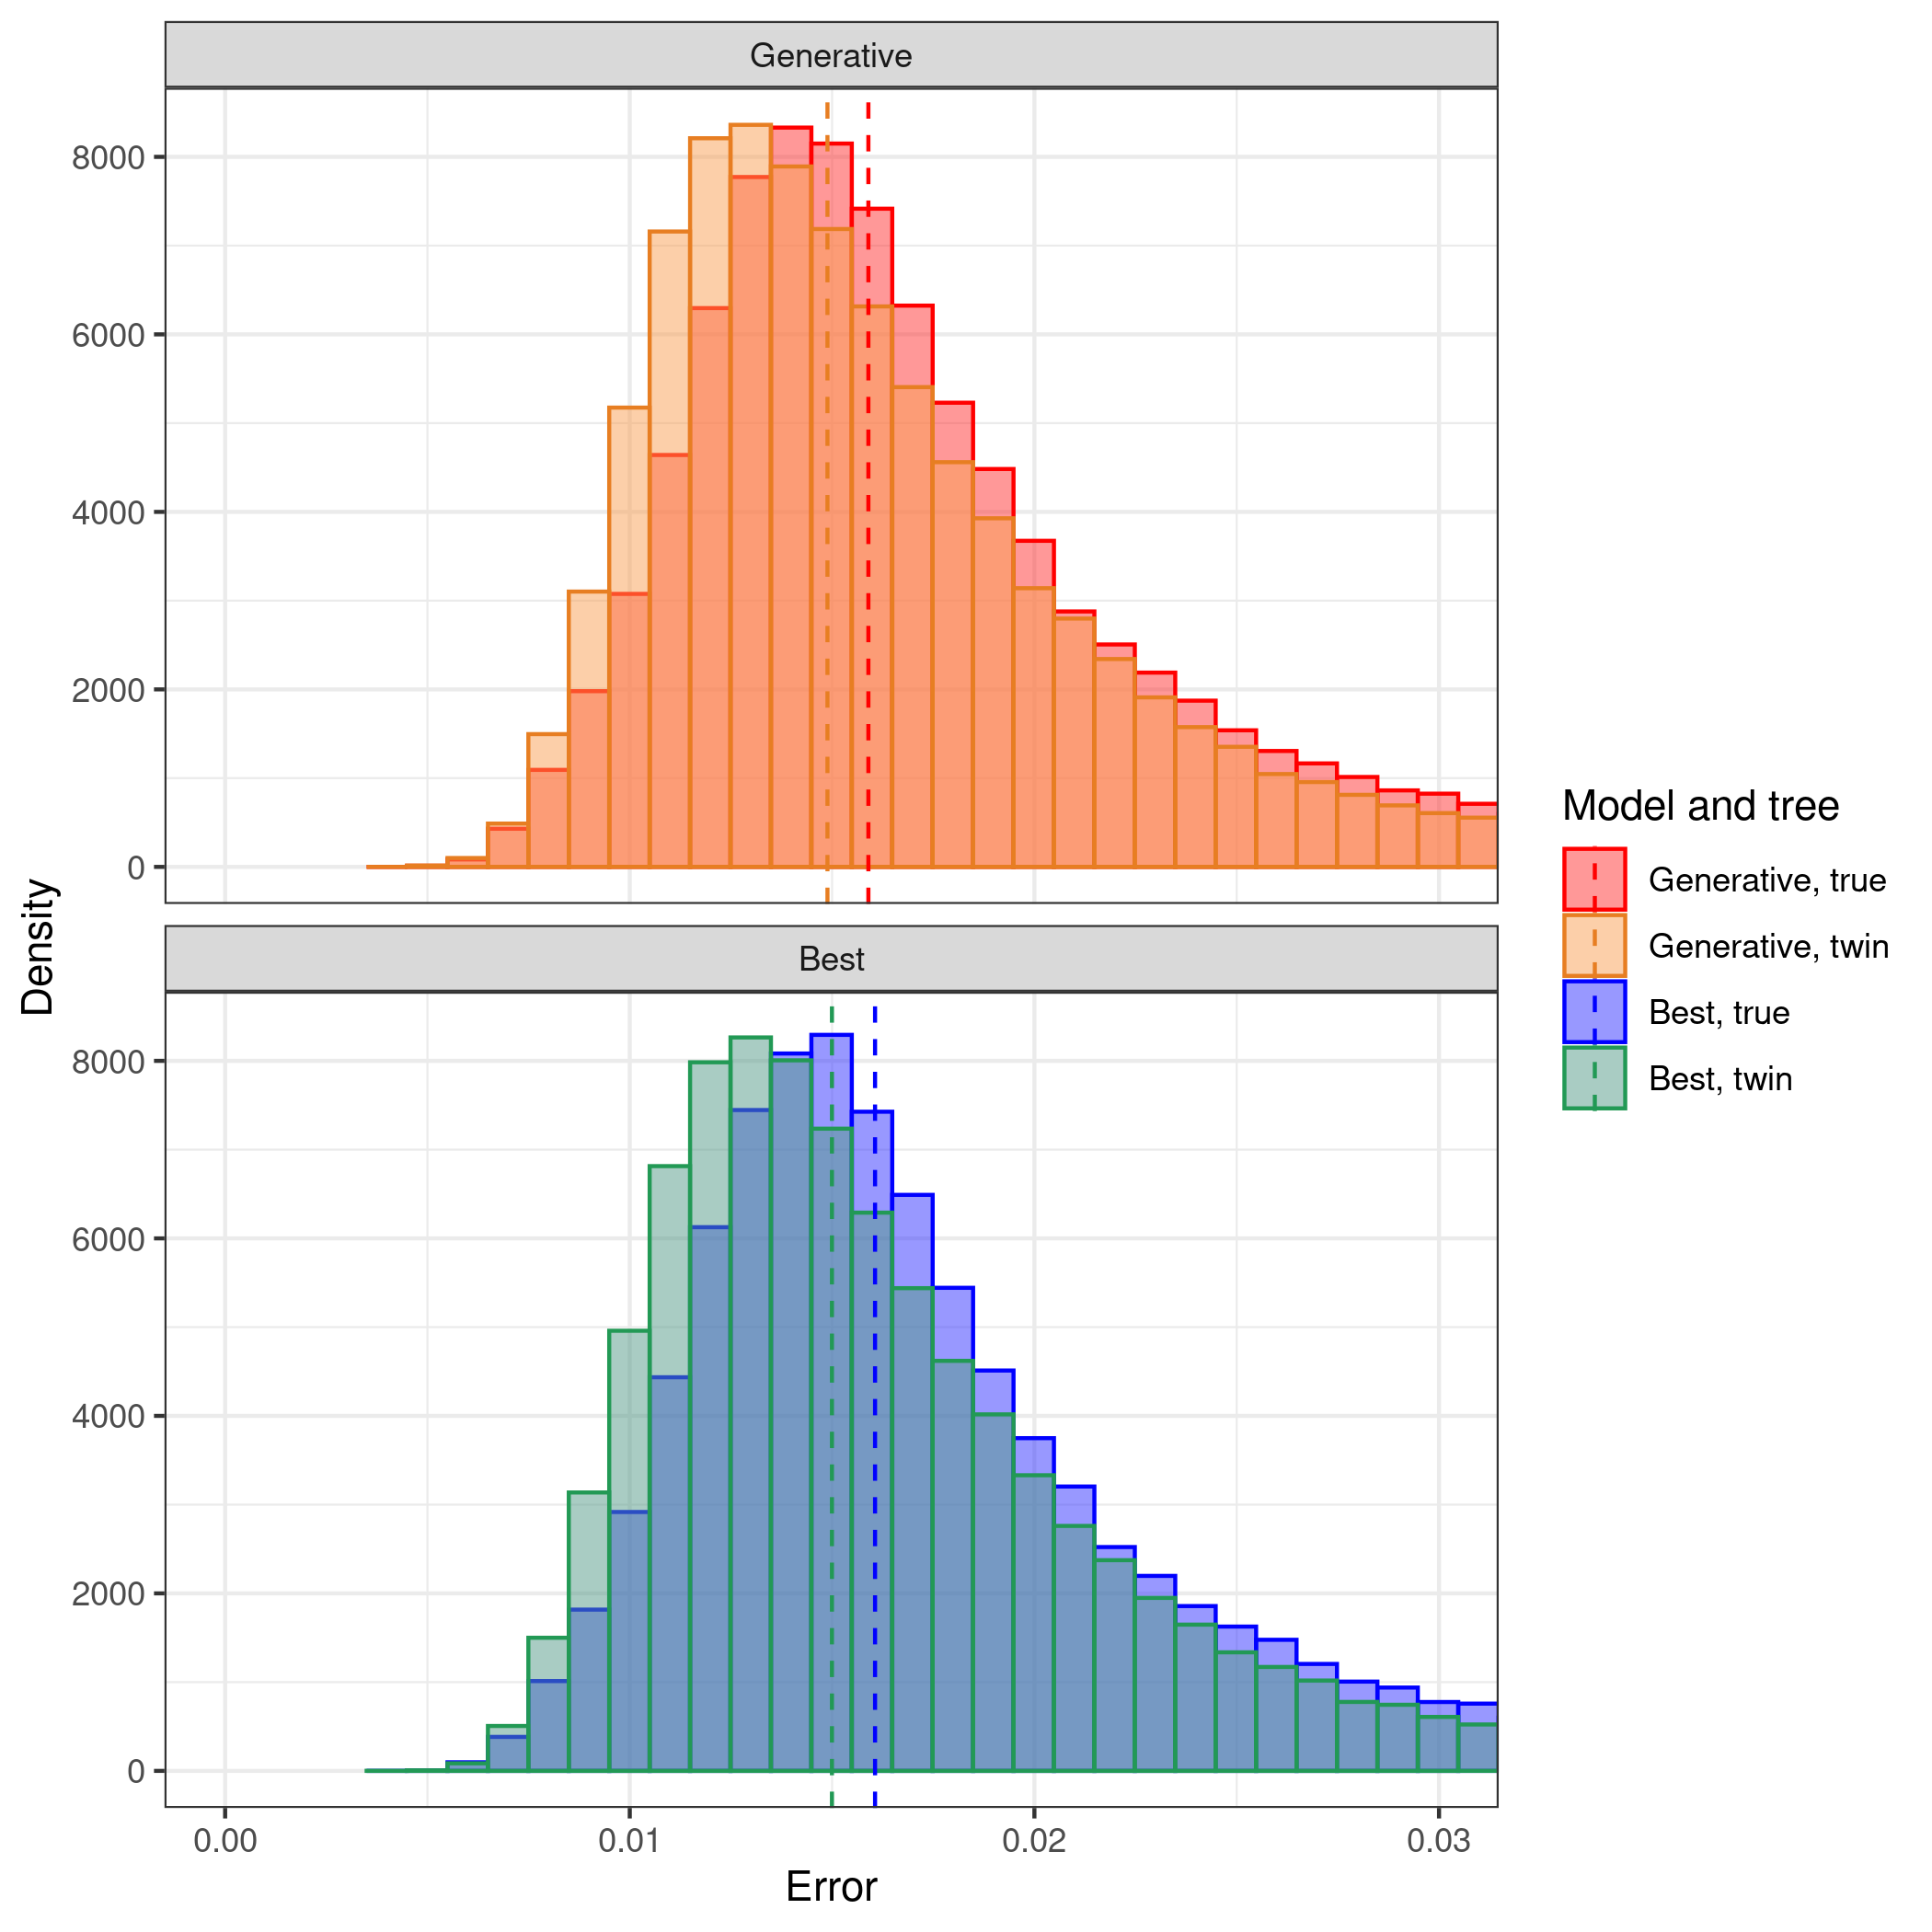
\includegraphics[width=0.98\textwidth]{pirouette_example_23/errors_low.png}
  \caption{Aggregate error distributions for a distribution of trees, where the true trees are DD with low likelihood.}
\end{figure}

\begin{figure}[H]
  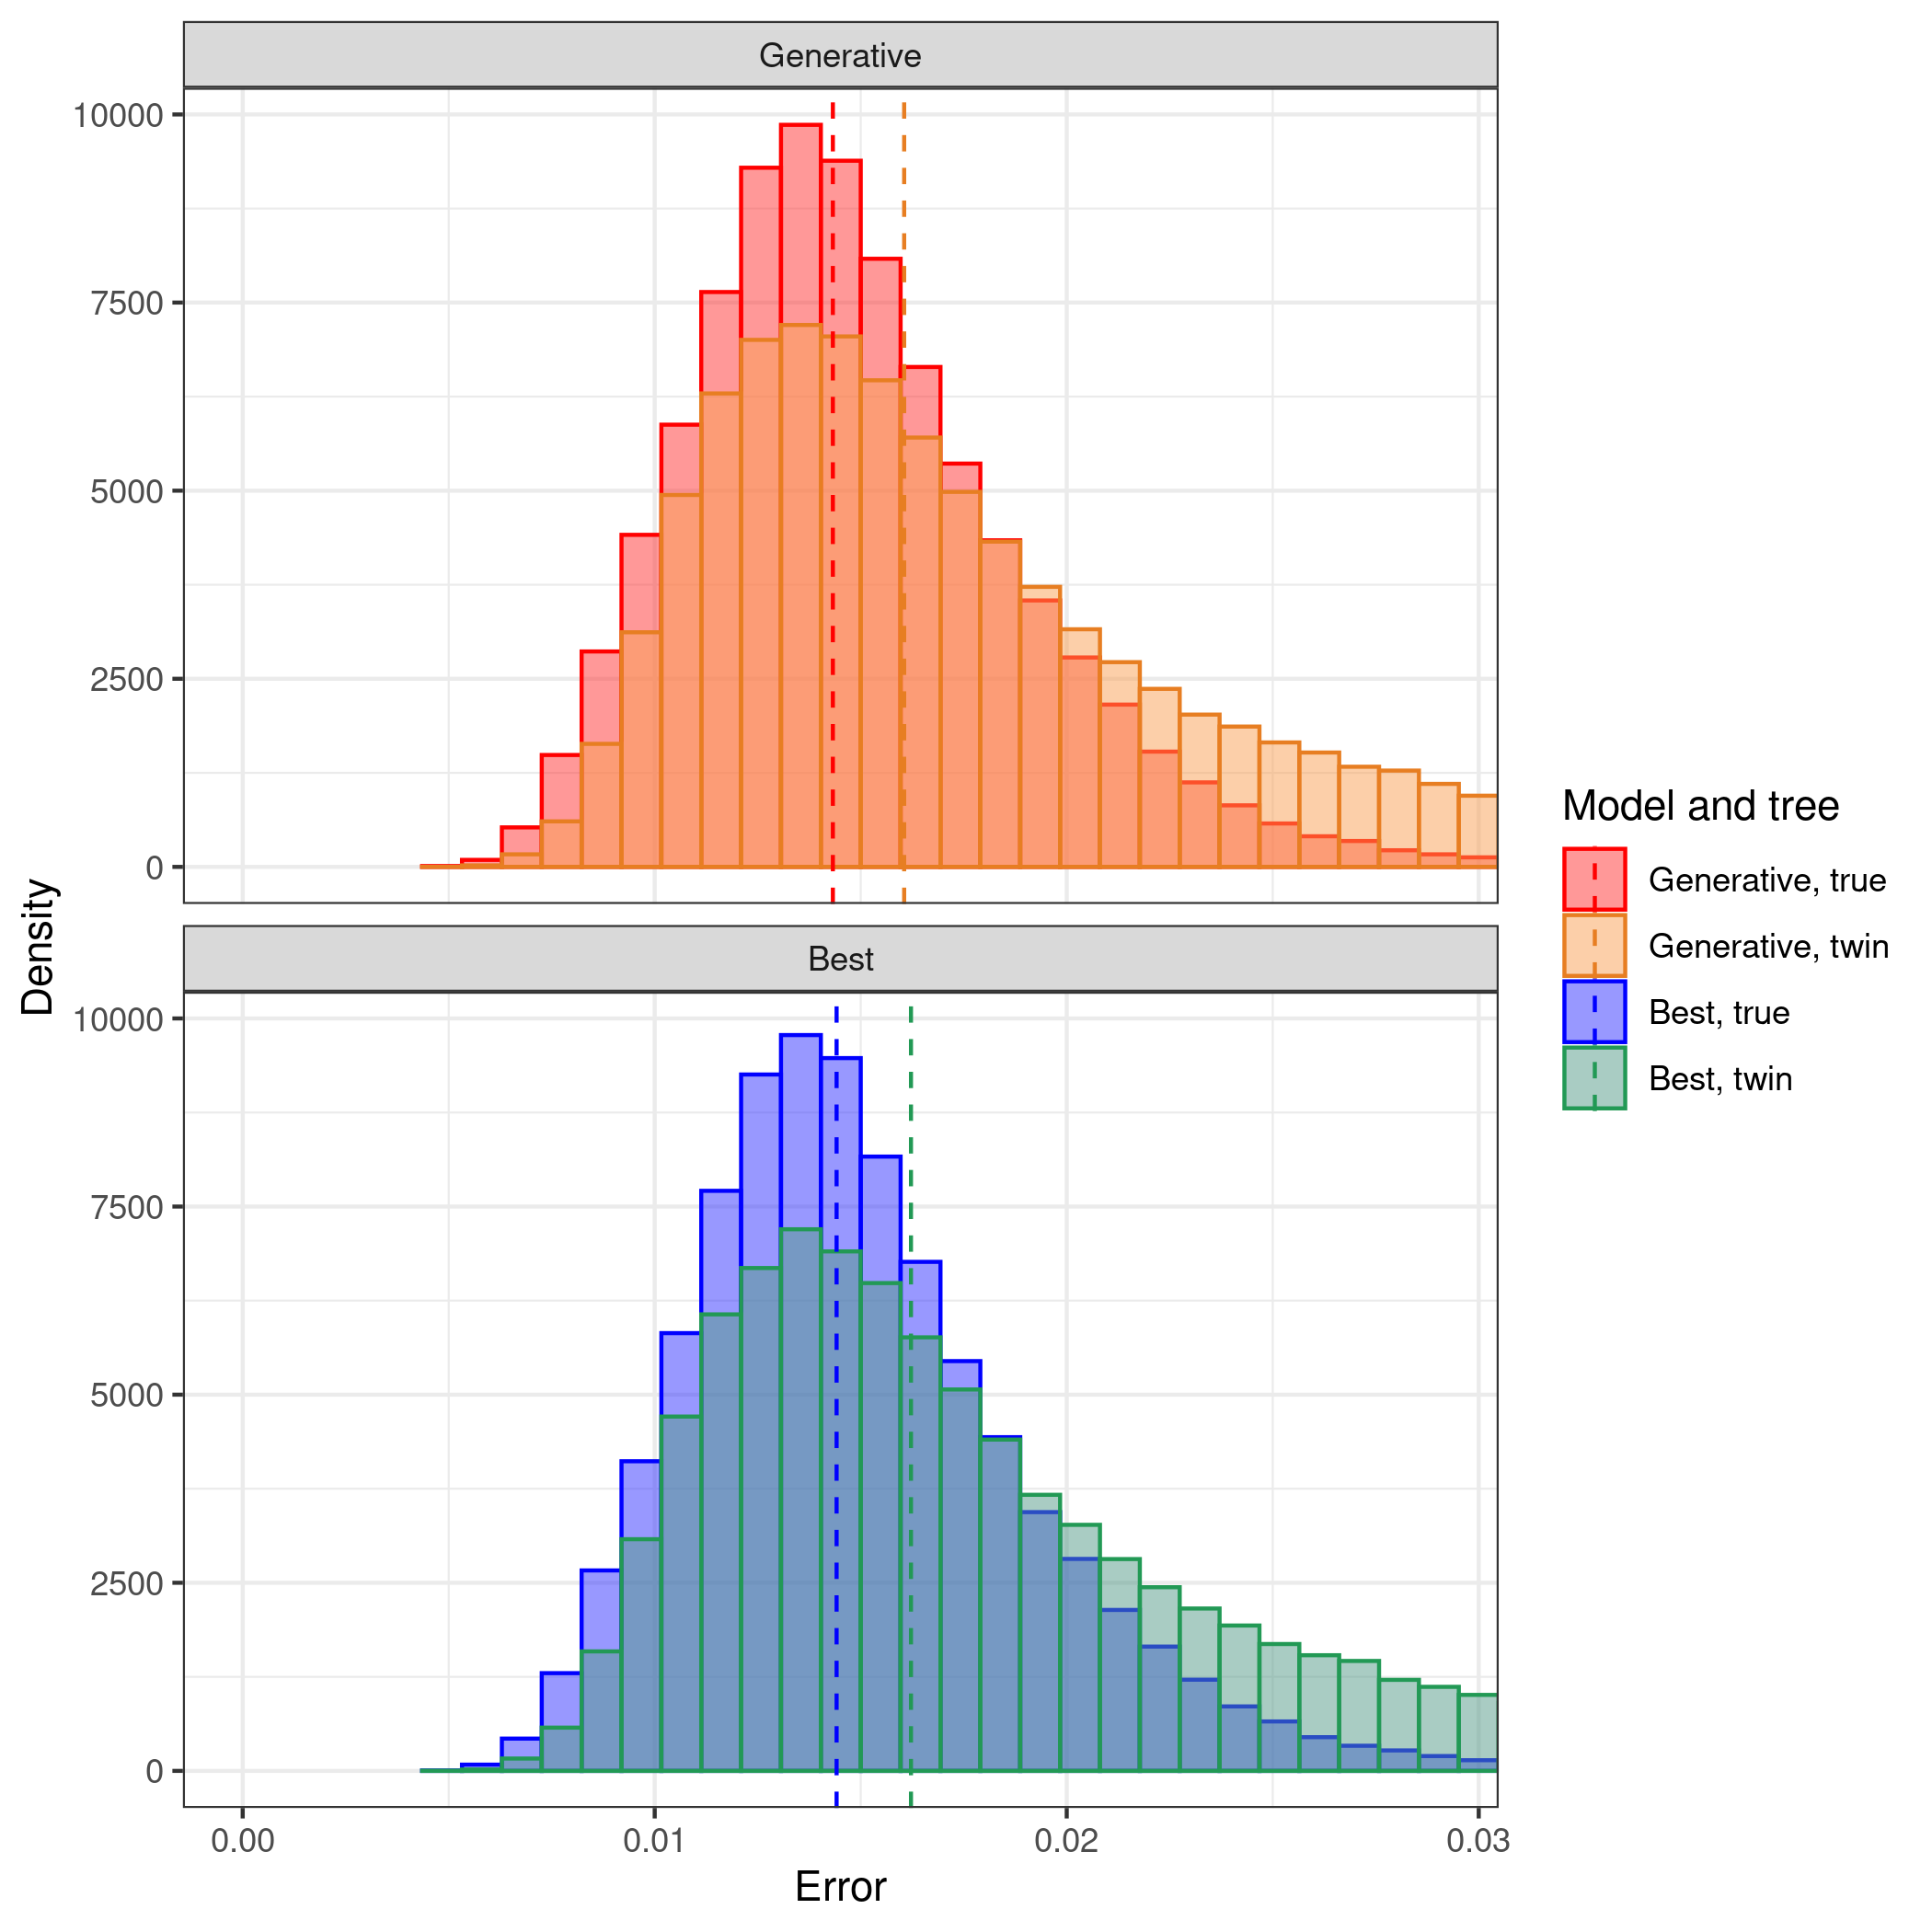
\includegraphics[width=0.98\textwidth]{pirouette_example_23/errors_mid.png}
  \caption{Aggregate error distributions for a distribution of trees, 
    where the true trees are DD with median likelihood.}
\end{figure}

\begin{figure}[H]
  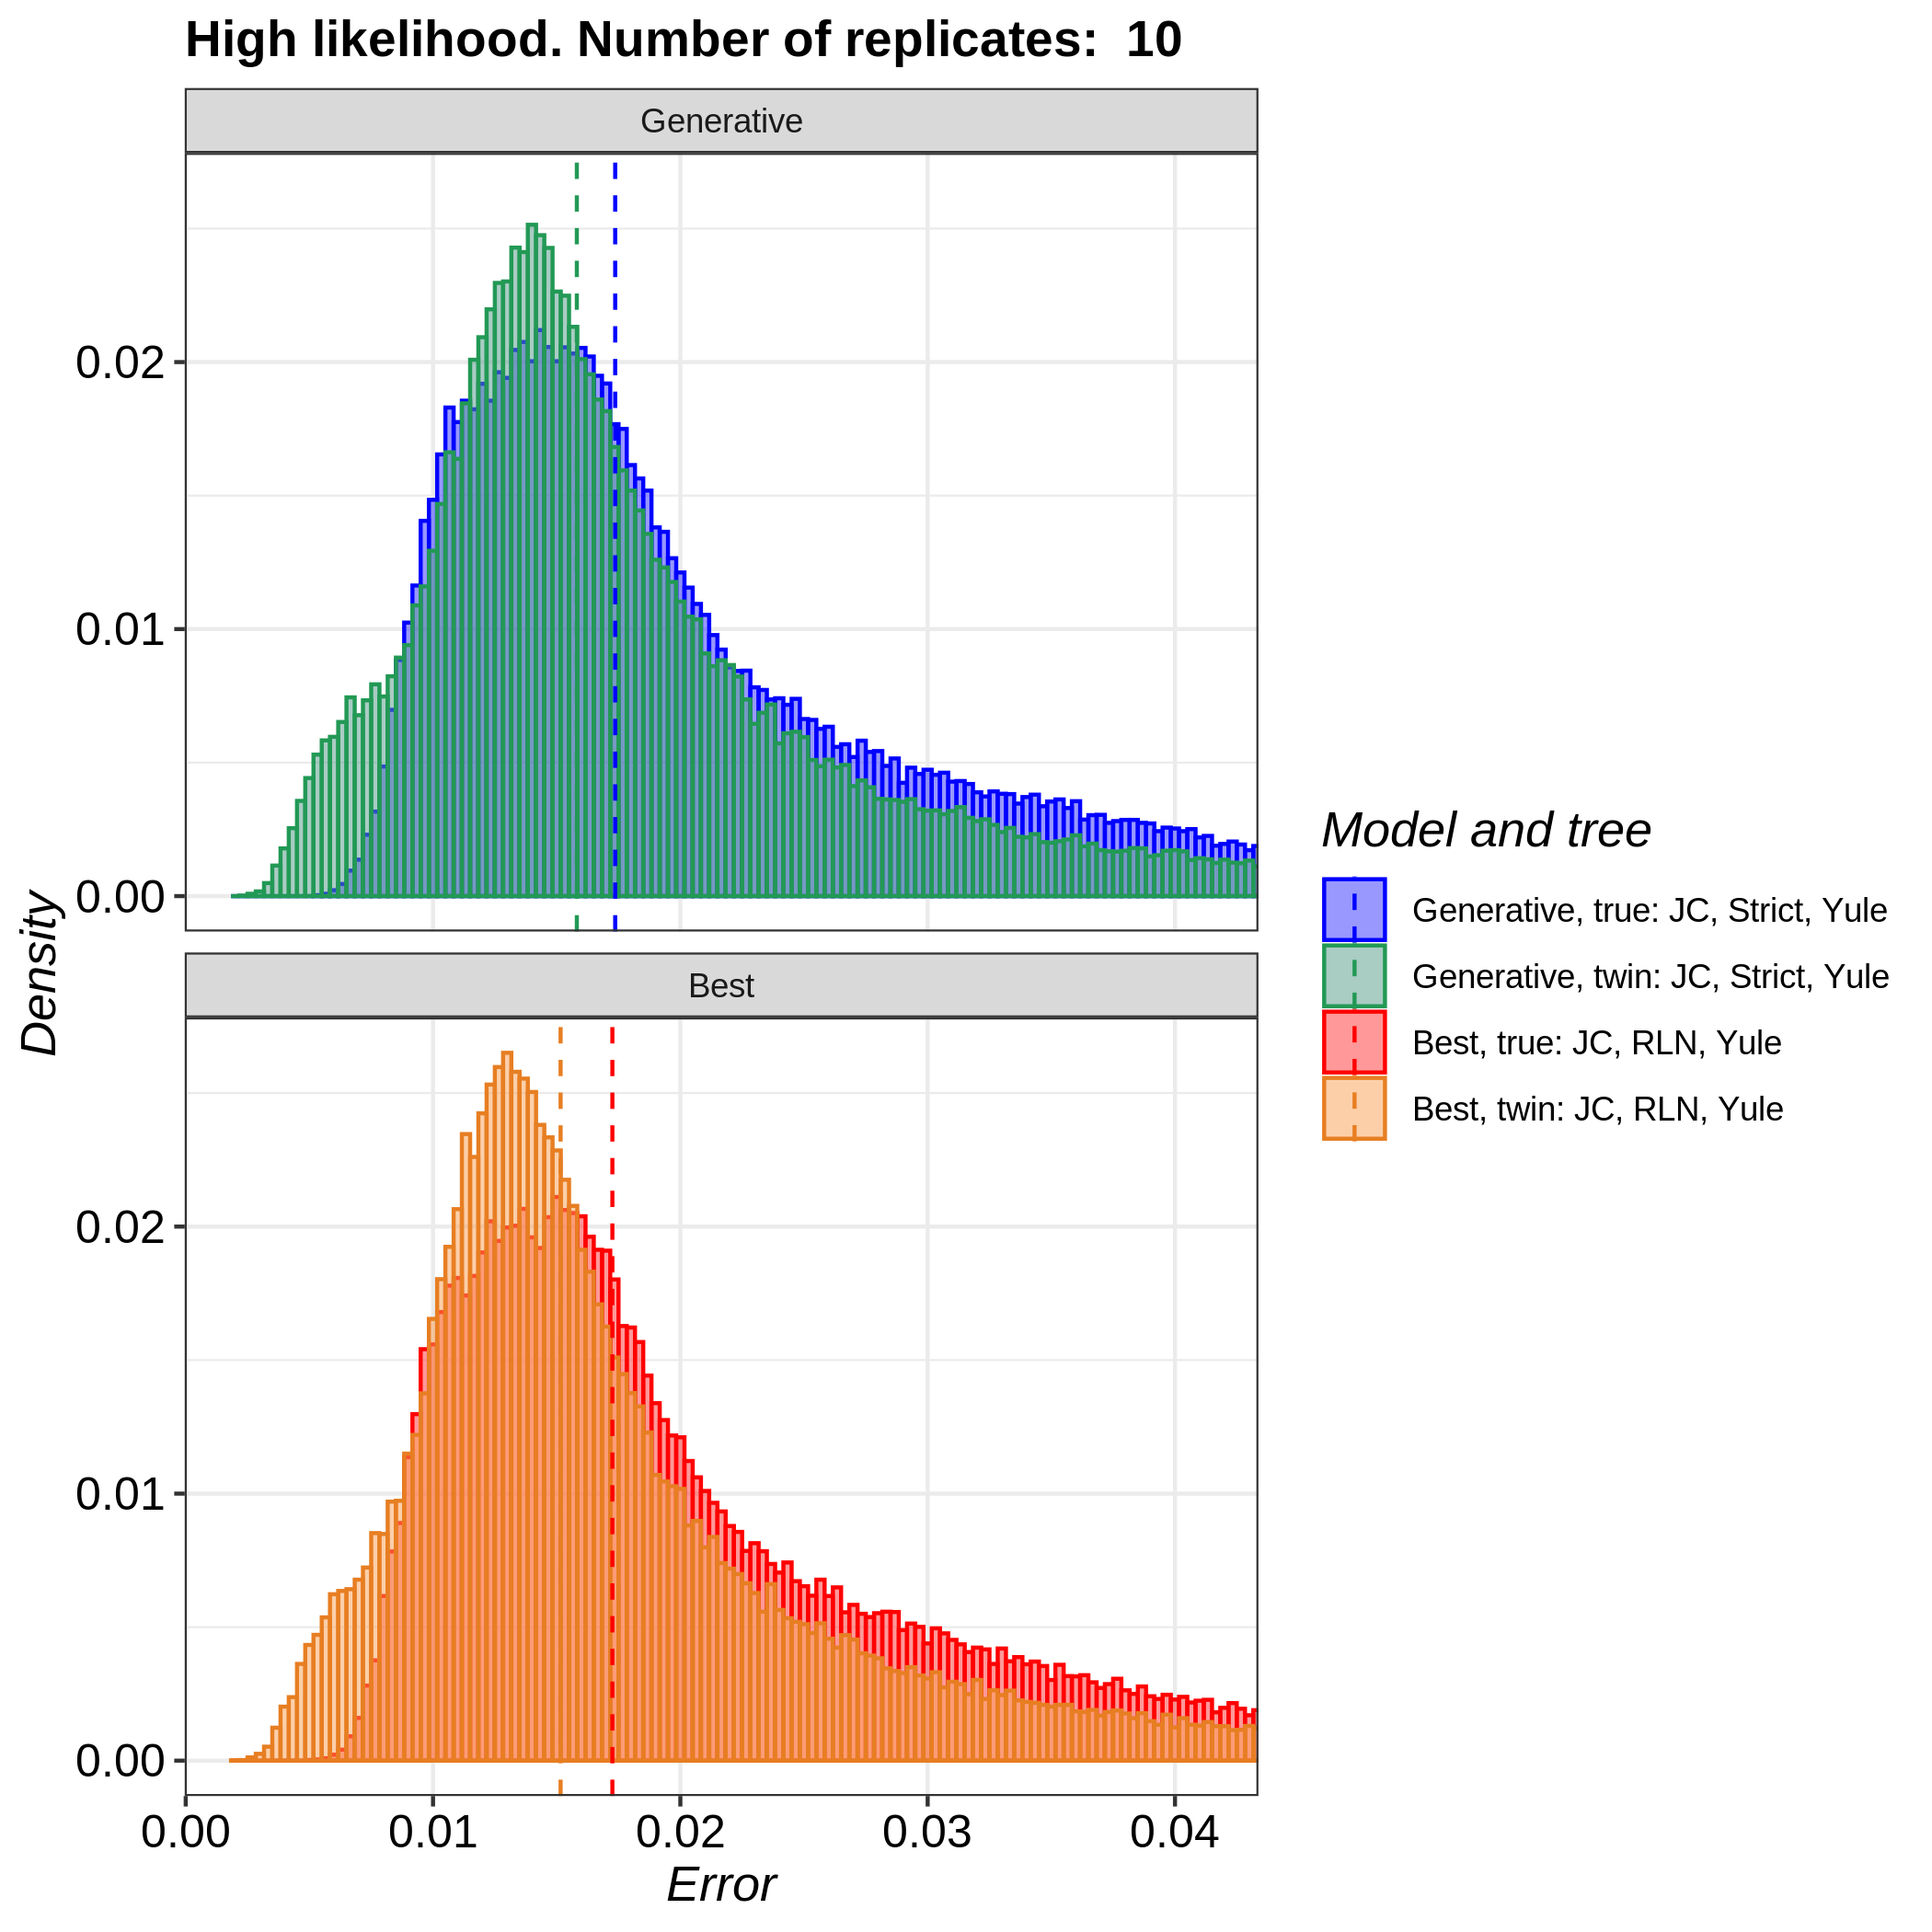
\includegraphics[width=0.98\textwidth]{pirouette_example_23/errors_high.png}
  \caption{
    Aggregate error distributions for a distribution of trees, 
    where the true trees are DD with high likelihood.
  }
\end{figure}

\new{
  Here the median errors are similar in the three settings and similar to 
  ones relative to the full dataset of \ref{subsec:distribution}. We can also 
  notice that in the case of median likelihood, the twin median error appears 
  to be lower than the true mean error. This is usually a sign that the number 
  of replicates (in this case 10) is too low to allow us to draw precise 
  conclusions from this test. We did not explore further in this 
  direction using more simulations because computational times turned to be 
  extremely high. 
  The entire run took 120 hours in total.
}

The code to reproduce these figure can be found at  
\begin{sloppypar}
  \url{https://github.com/richelbilderbeek/pirouette_example_23}
\end{sloppypar}.

\newpage

%%%%%%%%%%%%%%%%%%%%%%%%%%%%%%%%%%%%%%%%%%%%%%%%%%%%%%%%%%%%%%%%%%%%%%%%%%%%%%%%
\subsection{The effect of equal or equalized mutation rate in the twin alignment}
\label{subsec:different_n_mutations}
%%%%%%%%%%%%%%%%%%%%%%%%%%%%%%%%%%%%%%%%%%%%%%%%%%%%%%%%%%%%%%%%%%%%%%%%%%%%%%%%
  
The main example uses a twin alignment that has the same number
of \new{substitution}s (as measured from the ancestral sequence) as the true alignment. Here, we show the same results, with the difference that
the twin alignment uses the same mutation rate, yet is not guaranteed
to have the same number of \new{substitution}s.

\begin{figure}[H]
  %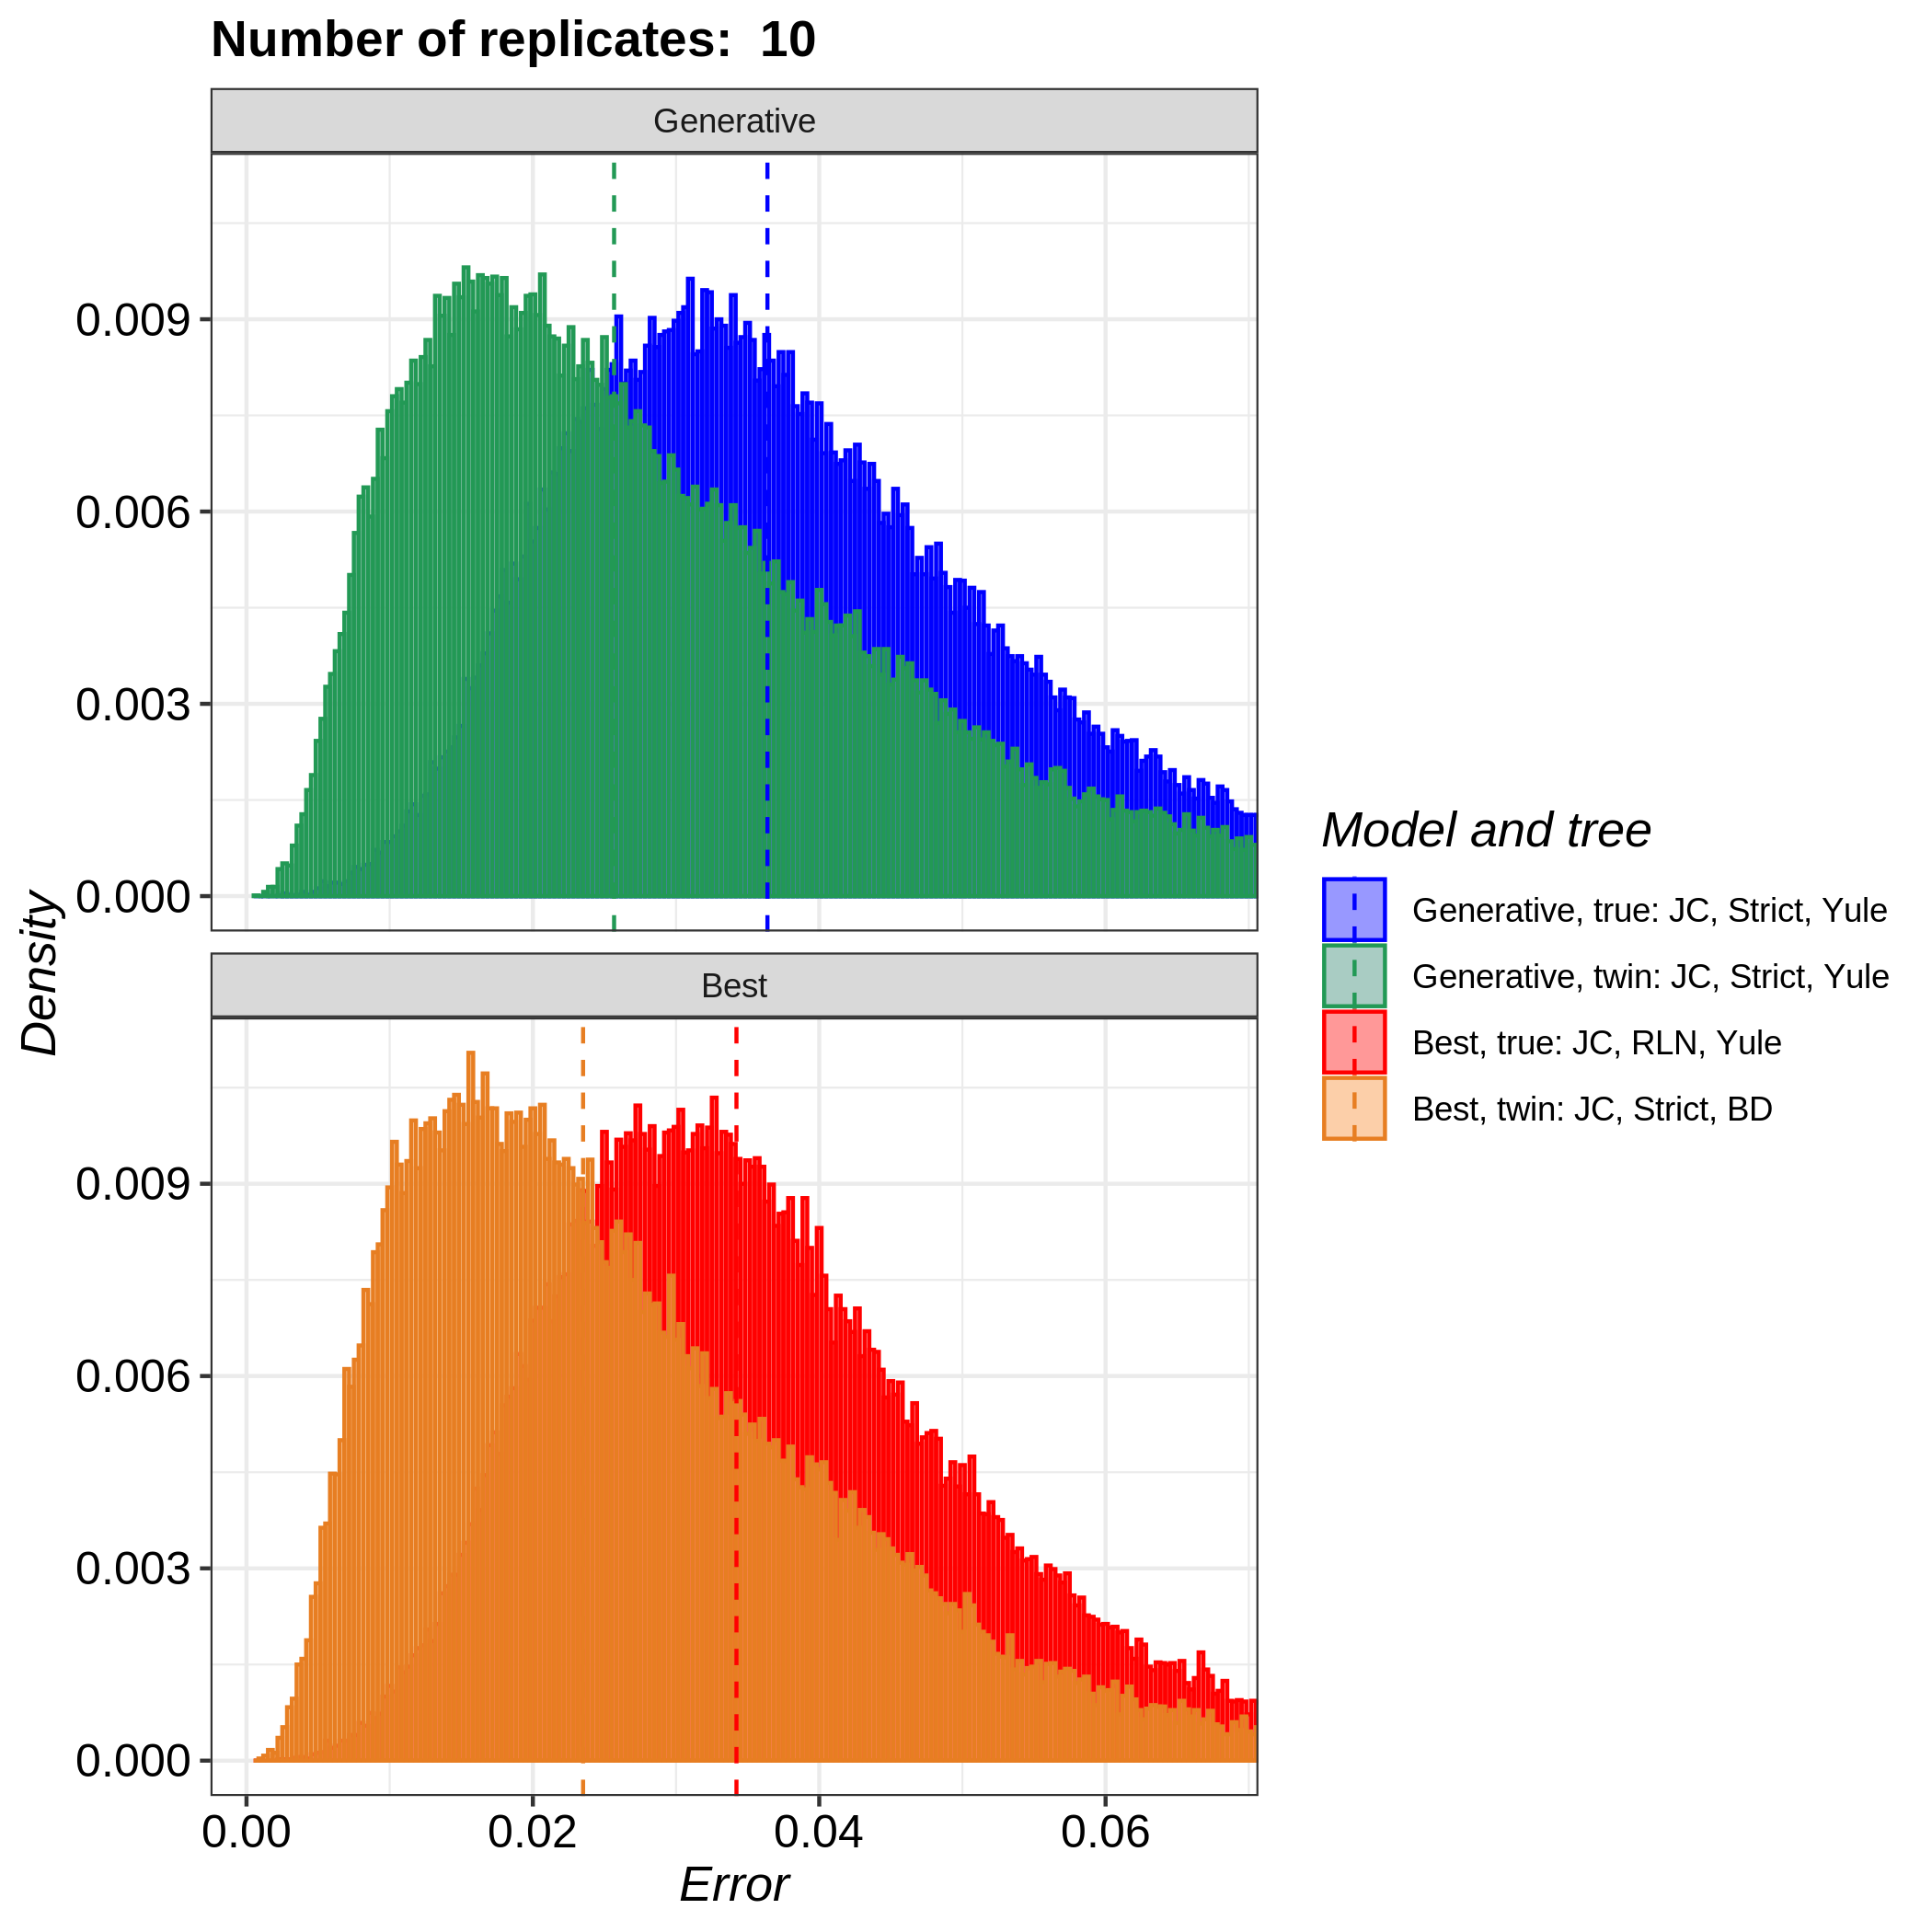
\includegraphics[width=0.98\textwidth]{pirouette_example_18/errors.png}
  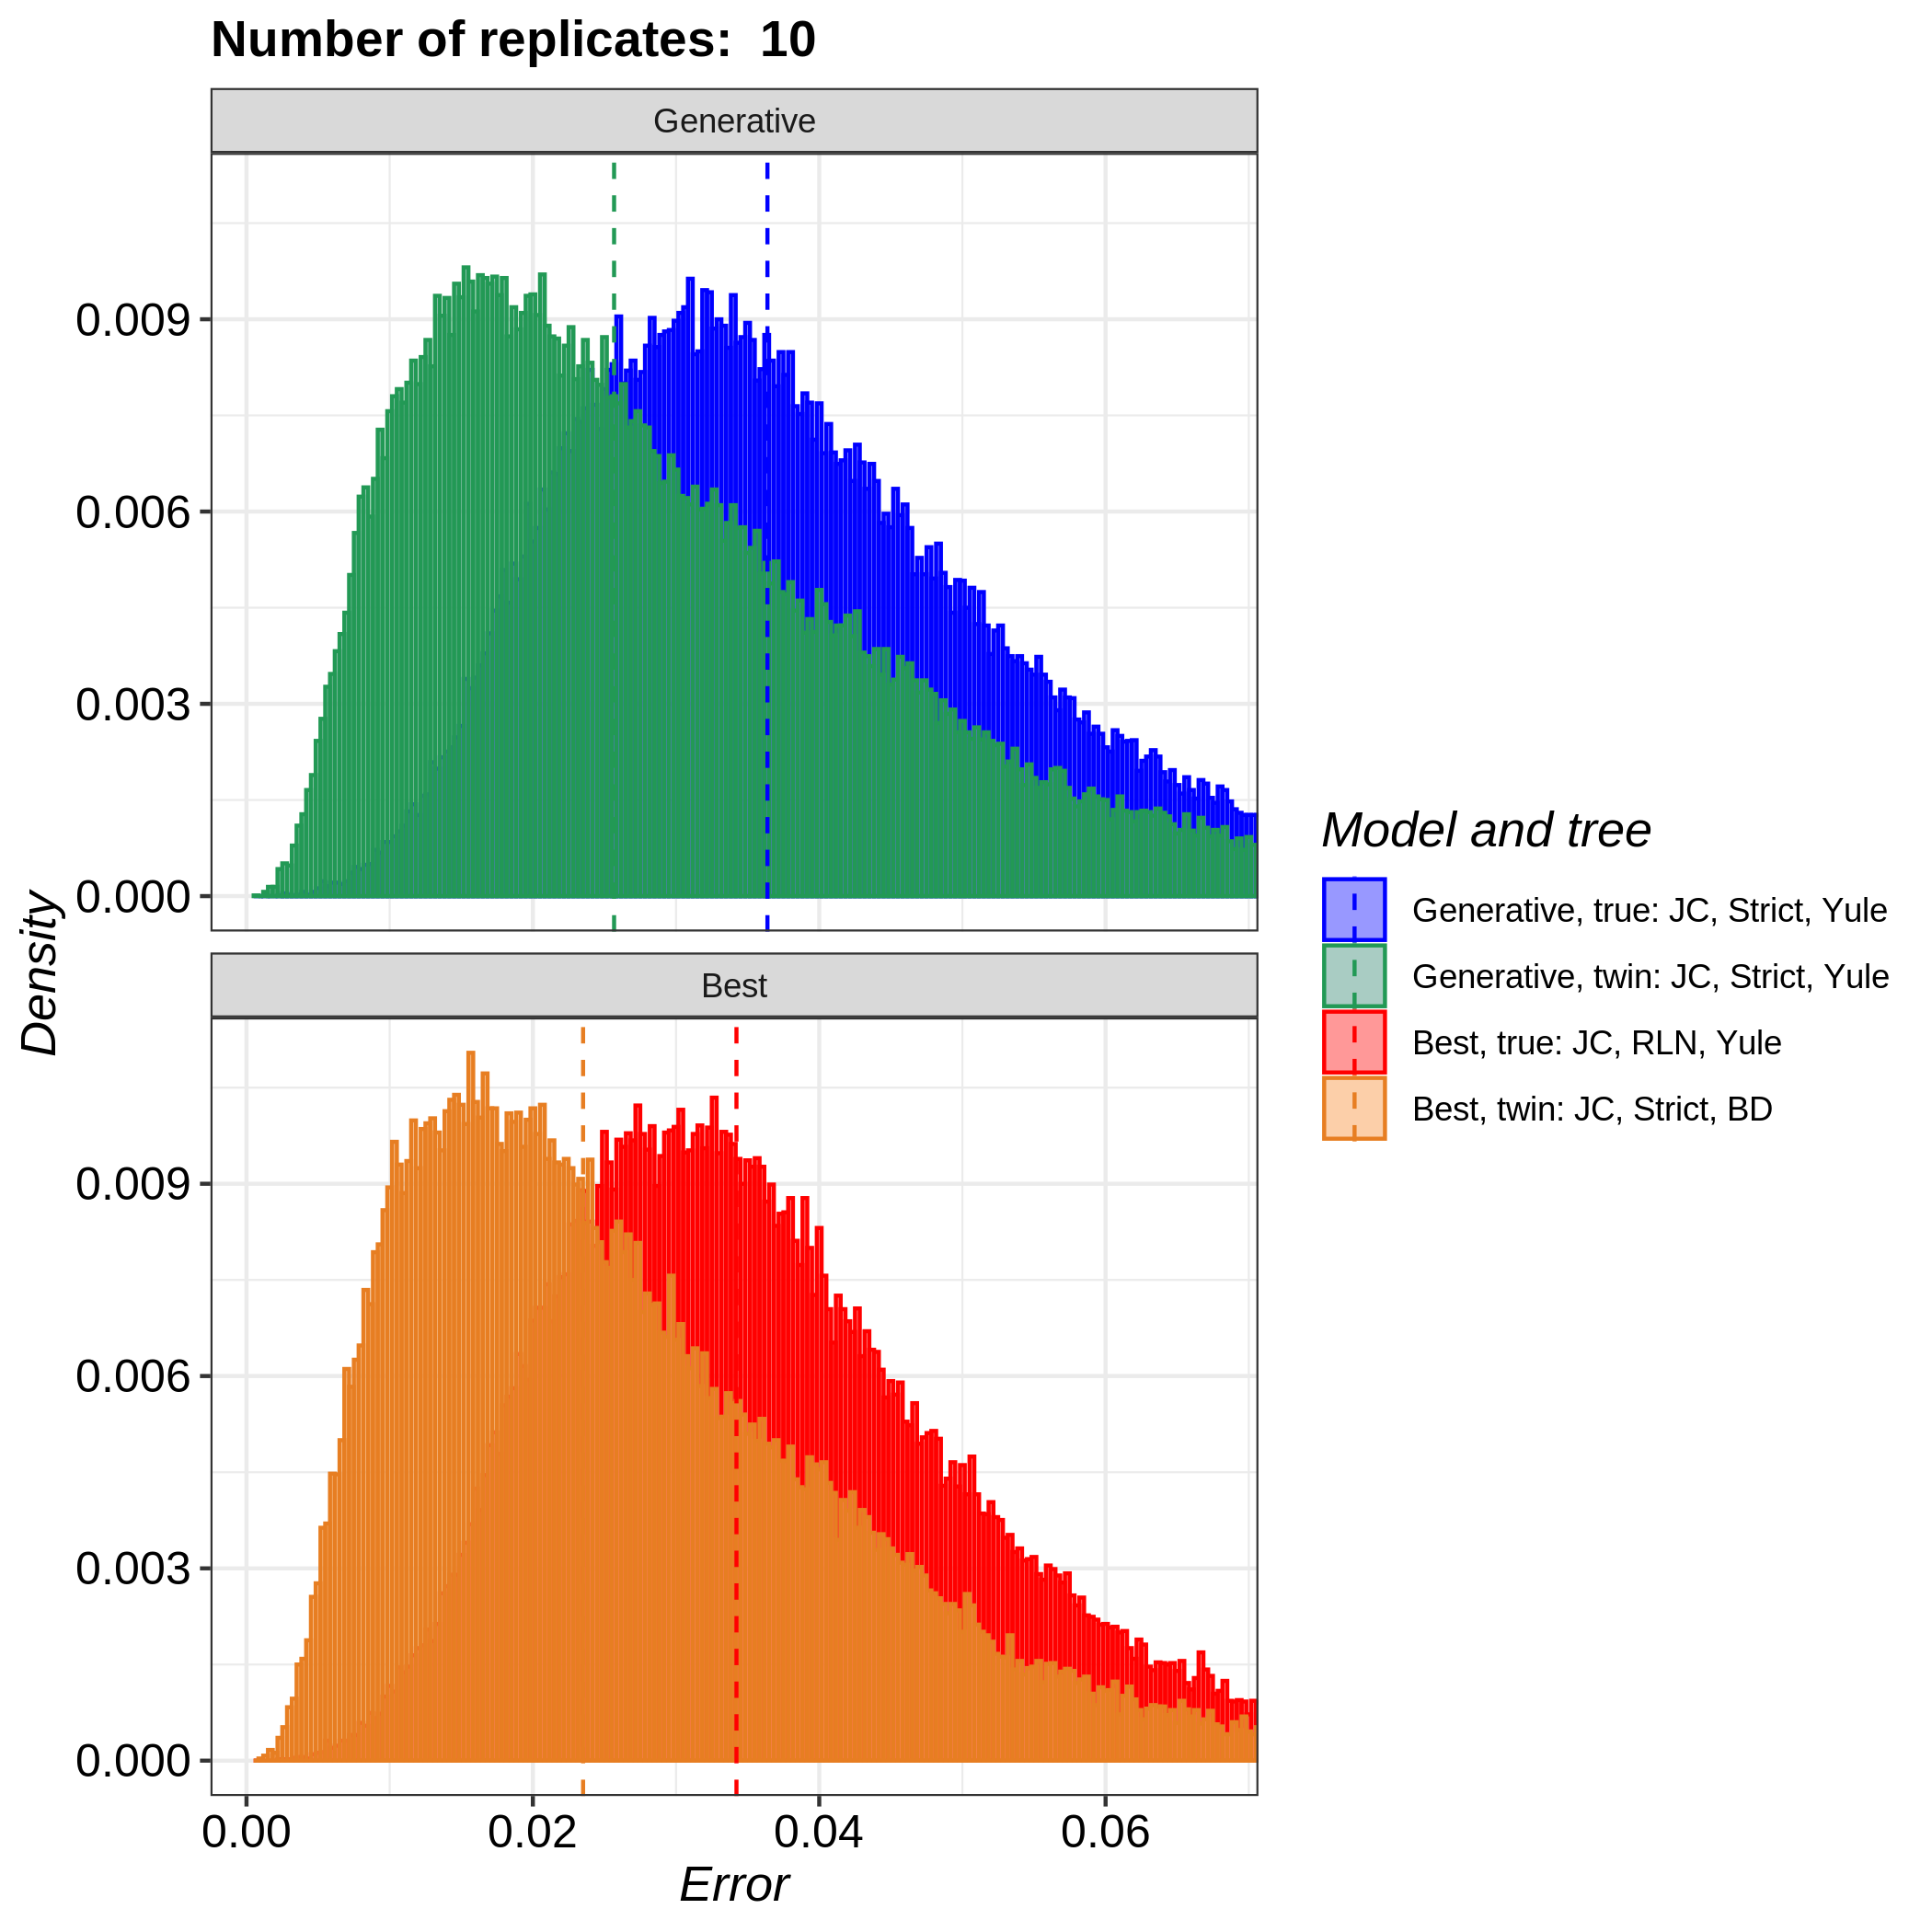
\includegraphics[width=0.94\textwidth]{pirouette_example_18/errors.png}
  \caption{Aggregate error distributions for 100 replicates.
    similar to Fig. \ref{fig:replicate_trees}, 
    but here the number of \new{substitution}s is not imposed 
    to be the same between true and twin alignment. 
    Instead, an equal mutation rate is used. 
    This took 3.3 days (wall clock time) to compute.}
  \label{fig:example_random_mutations}
\end{figure}

\new{
  Comparing figures \ref{fig:example_random_mutations} 
  and \ref{fig:replicate_trees} we can see that the discrepancy between 
  true and twin distributions tend to increase. 
  This is probably due to the fact that letting mutation rates 
  induces a difference in the amount of information contained in the 
  alignments and this is reflected in the error distributions.
}

The code to reproduce this figure can be found at
\begin{sloppypar}
  \url{https://github.com/richelbilderbeek/pirouette_example_18} and
  \url{https://github.com/richelbilderbeek/pirouette_example_28}.
\end{sloppypar}

\newpage

%%%%%%%%%%%%%%%%%%%%%%%%%%%%%%%%%%%%%%%%%%%%%%%%%%%%%%%%%%%%%%%%%%%%%%%%%%%%%%%%
\subsection{The effect of mutation rate}
\label{subsec:mutation_rate}
%%%%%%%%%%%%%%%%%%%%%%%%%%%%%%%%%%%%%%%%%%%%%%%%%%%%%%%%%%%%%%%%%%%%%%%%%%%%%%%%

The main example uses a mutation rate such that all nucleotides,
on average, mutate once over the history going from the
ancestral sequence at the crown to the alignments at the tips.
This value equals `1.0 / crown age`.
In this way, the alignment is expected to contain the maximum
amount of information.

Here, we show the same results for different mutation rates.
\new{
\iffalse
  We can observe that the error tends to increases for mutation rates above
  `1.0 / crown age`. Below this value, the errors are the same.
  For these lower mutation rates, however, the shape of the error
  distribution changes for the baseline/generative models,
  deviating more and more from the gamma-distribution-like shape
  as is still present in the twin distributions.
\fi
 The results for the different mutation rates are shown in Figs. \ref{fig:example_0.25_mutation_rate} (0.25 / crown age), \ref{fig:example_0.50_mutation_rate} (0.50 / crown age), \ref{fig:example_0.75_mutation_rate} (0.75 / crown age), \ref{fig:replicate_trees} (1.00 / crown age), \ref{fig:example_1.25_mutation_rate} (1.25 / crown age),
 \ref{fig:example_1.50_mutation_rate} (1.50 / crown age) and
 \ref{fig:example_2.00_mutation_rate} (2.00 / crown age).
 }
\new{
 Fig. \ref{fig:error_vs_mutationrate} summarizes all the other figures showing on the y-axis, for each value of the mutation rate, the difference between the median of the true distribution and the median of the twin distribution. We can observe a general positive trend as the mutation rate increase, even though the value for 1.5 / crown age suggests to take this result with caution. It is possible, however, that a more regular trend could be observed increasing the number of simulations.
}

The code to reproduce this figure can be found at
\begin{sloppypar}
  \url{https://github.com/richelbilderbeek/pirouette_example_35} (0.25 / crown age),
  \url{https://github.com/richelbilderbeek/pirouette_example_36} (0.50 / crown age),
  \url{https://github.com/richelbilderbeek/pirouette_example_37} (0.75 / crown age),
  \url{https://github.com/richelbilderbeek/pirouette_example_28} (1.00 / crown age, example reported in \ref{subsec:distribution}, see Fig. \ref{fig:replicate_trees}),
  \url{https://github.com/richelbilderbeek/pirouette_example_38} (1.25 / crown age),
  \url{https://github.com/richelbilderbeek/pirouette_example_39} (1.50 / crown age),
  \url{https://github.com/richelbilderbeek/pirouette_example_40} (2.00 / crown age),
\end{sloppypar}

\begin{figure}[H]
  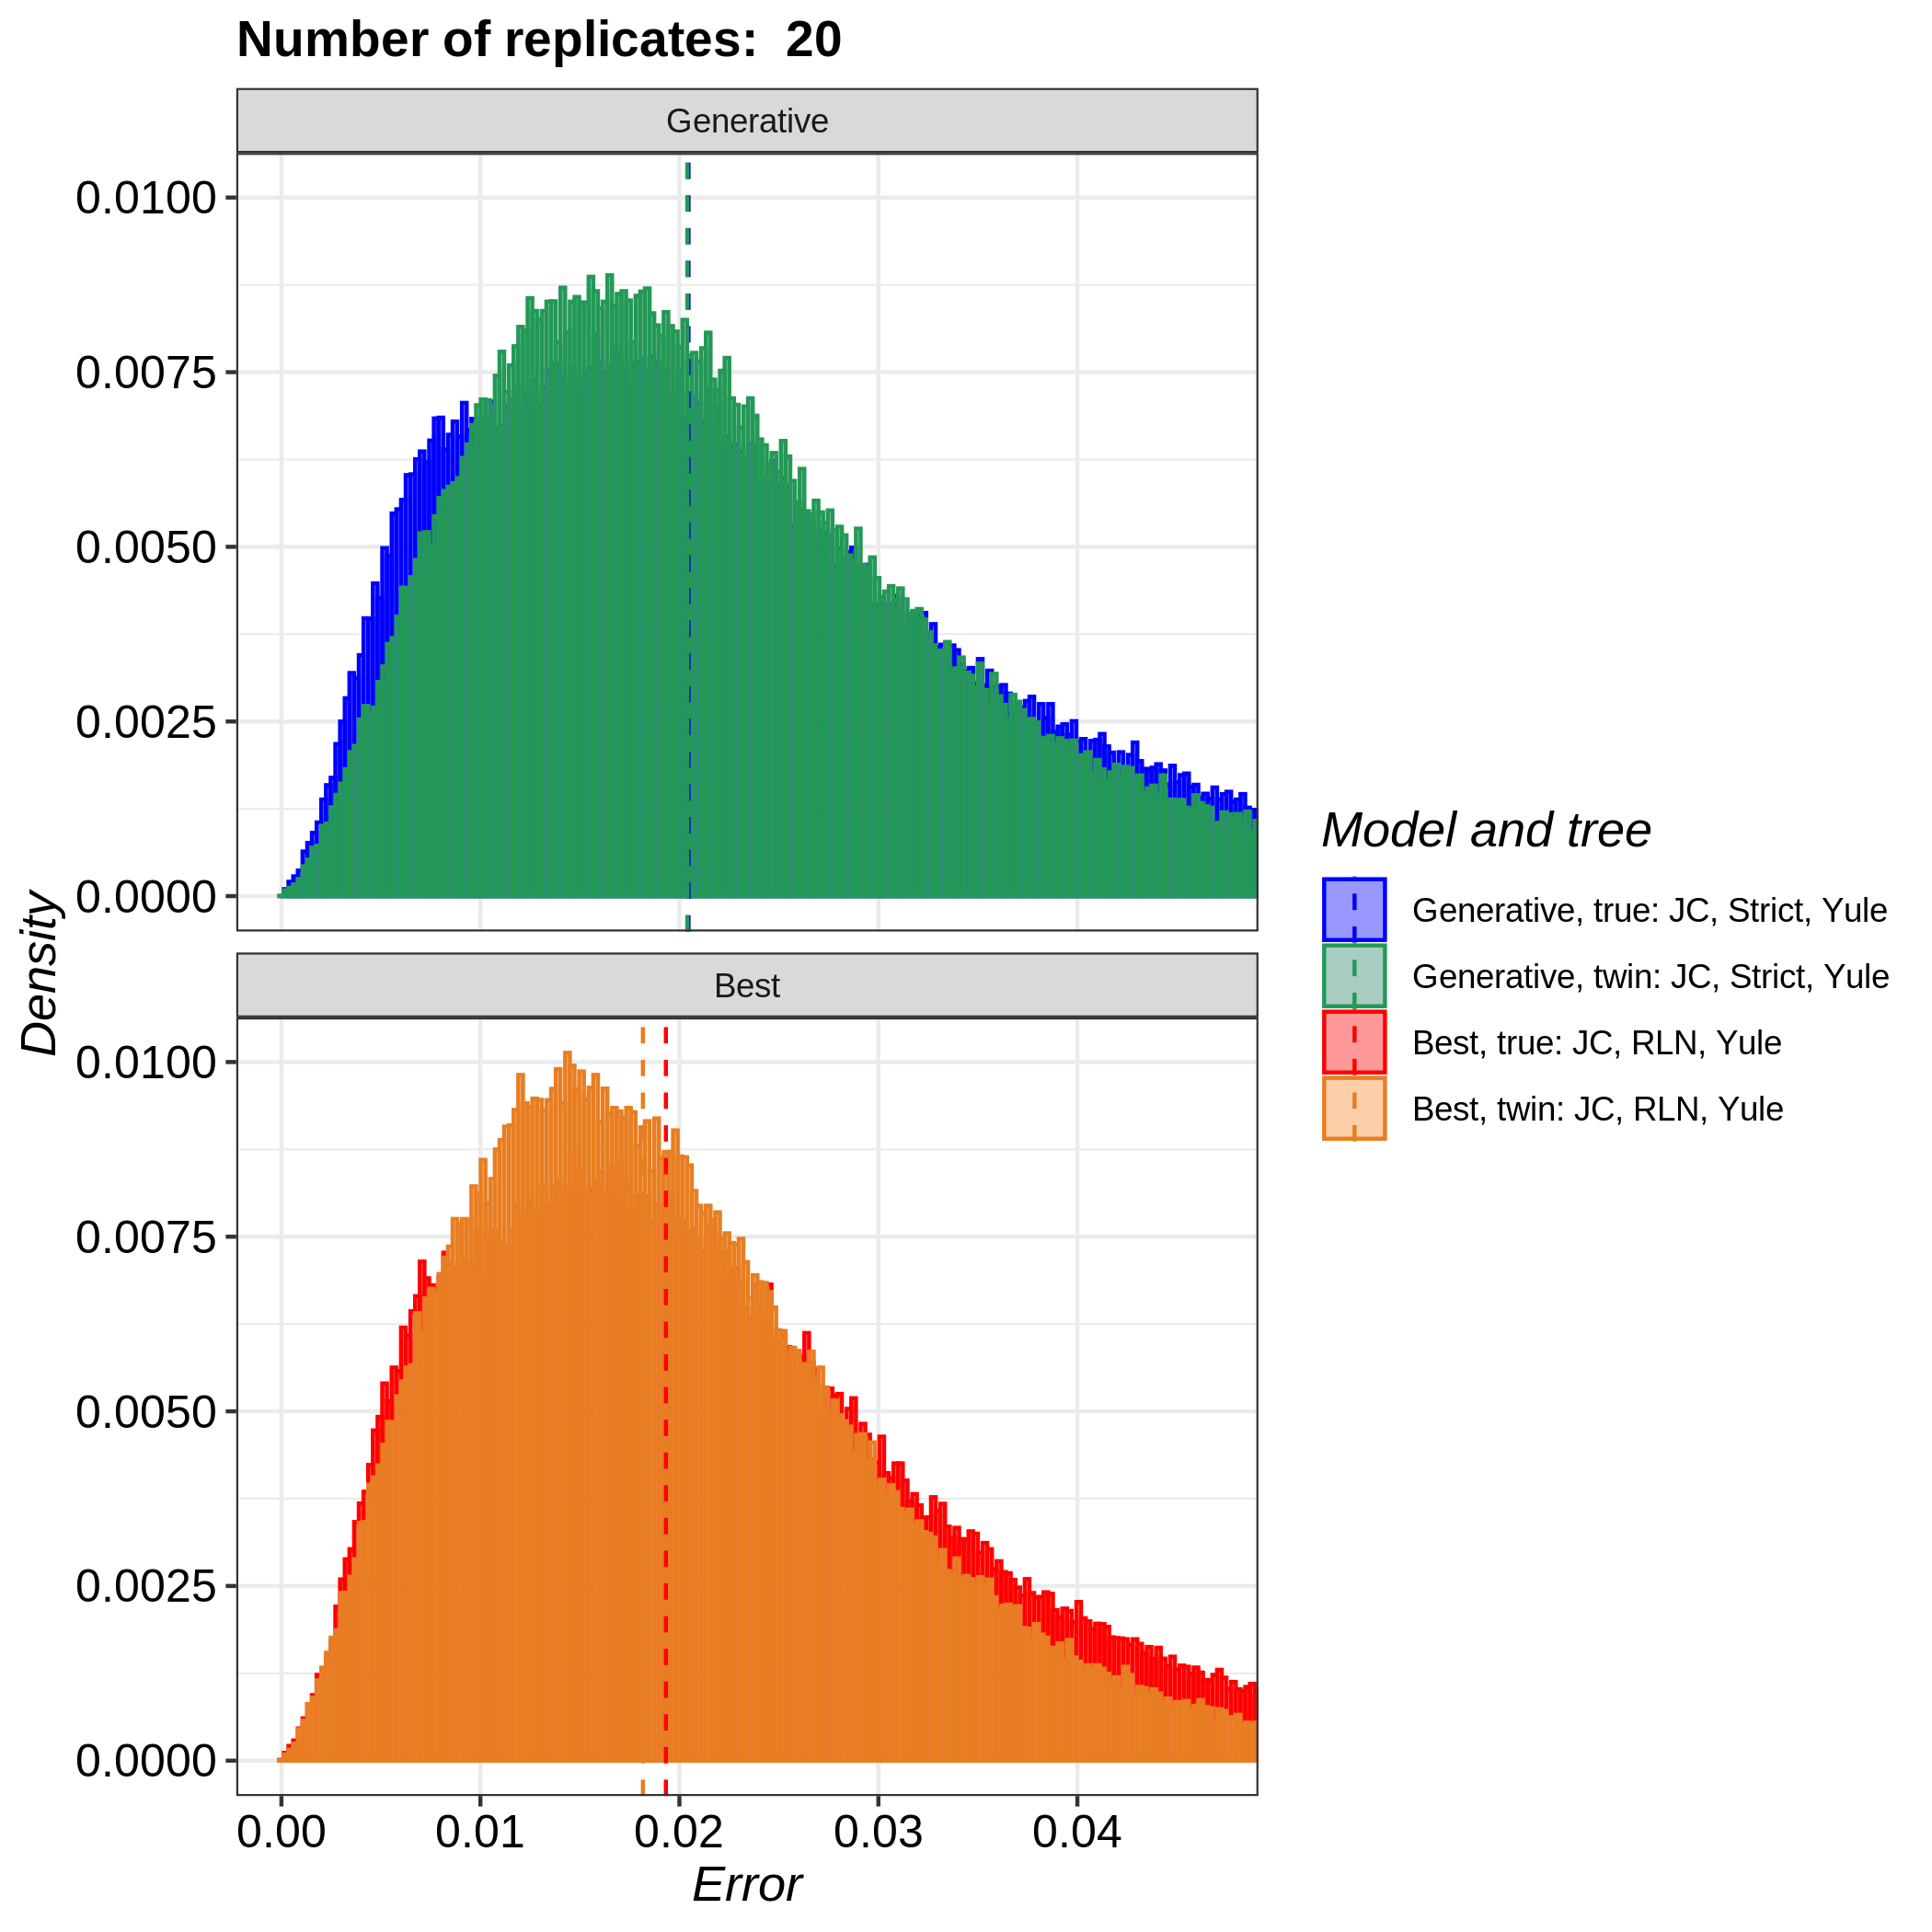
\includegraphics[width=0.98\textwidth]{pirouette_example_35/errors.png}
  \caption{Aggregate error distributions for 100 replicates,
    for the tree distribution presented 
    in \ref{subsec:distribution} but with a per-nucleotide mutation rate 
    of 0.25 / crown age. 
    This took 1.8 days (wall clock time) to compute.}
  \label{fig:example_0.25_mutation_rate}
\end{figure}

\begin{figure}[H]
  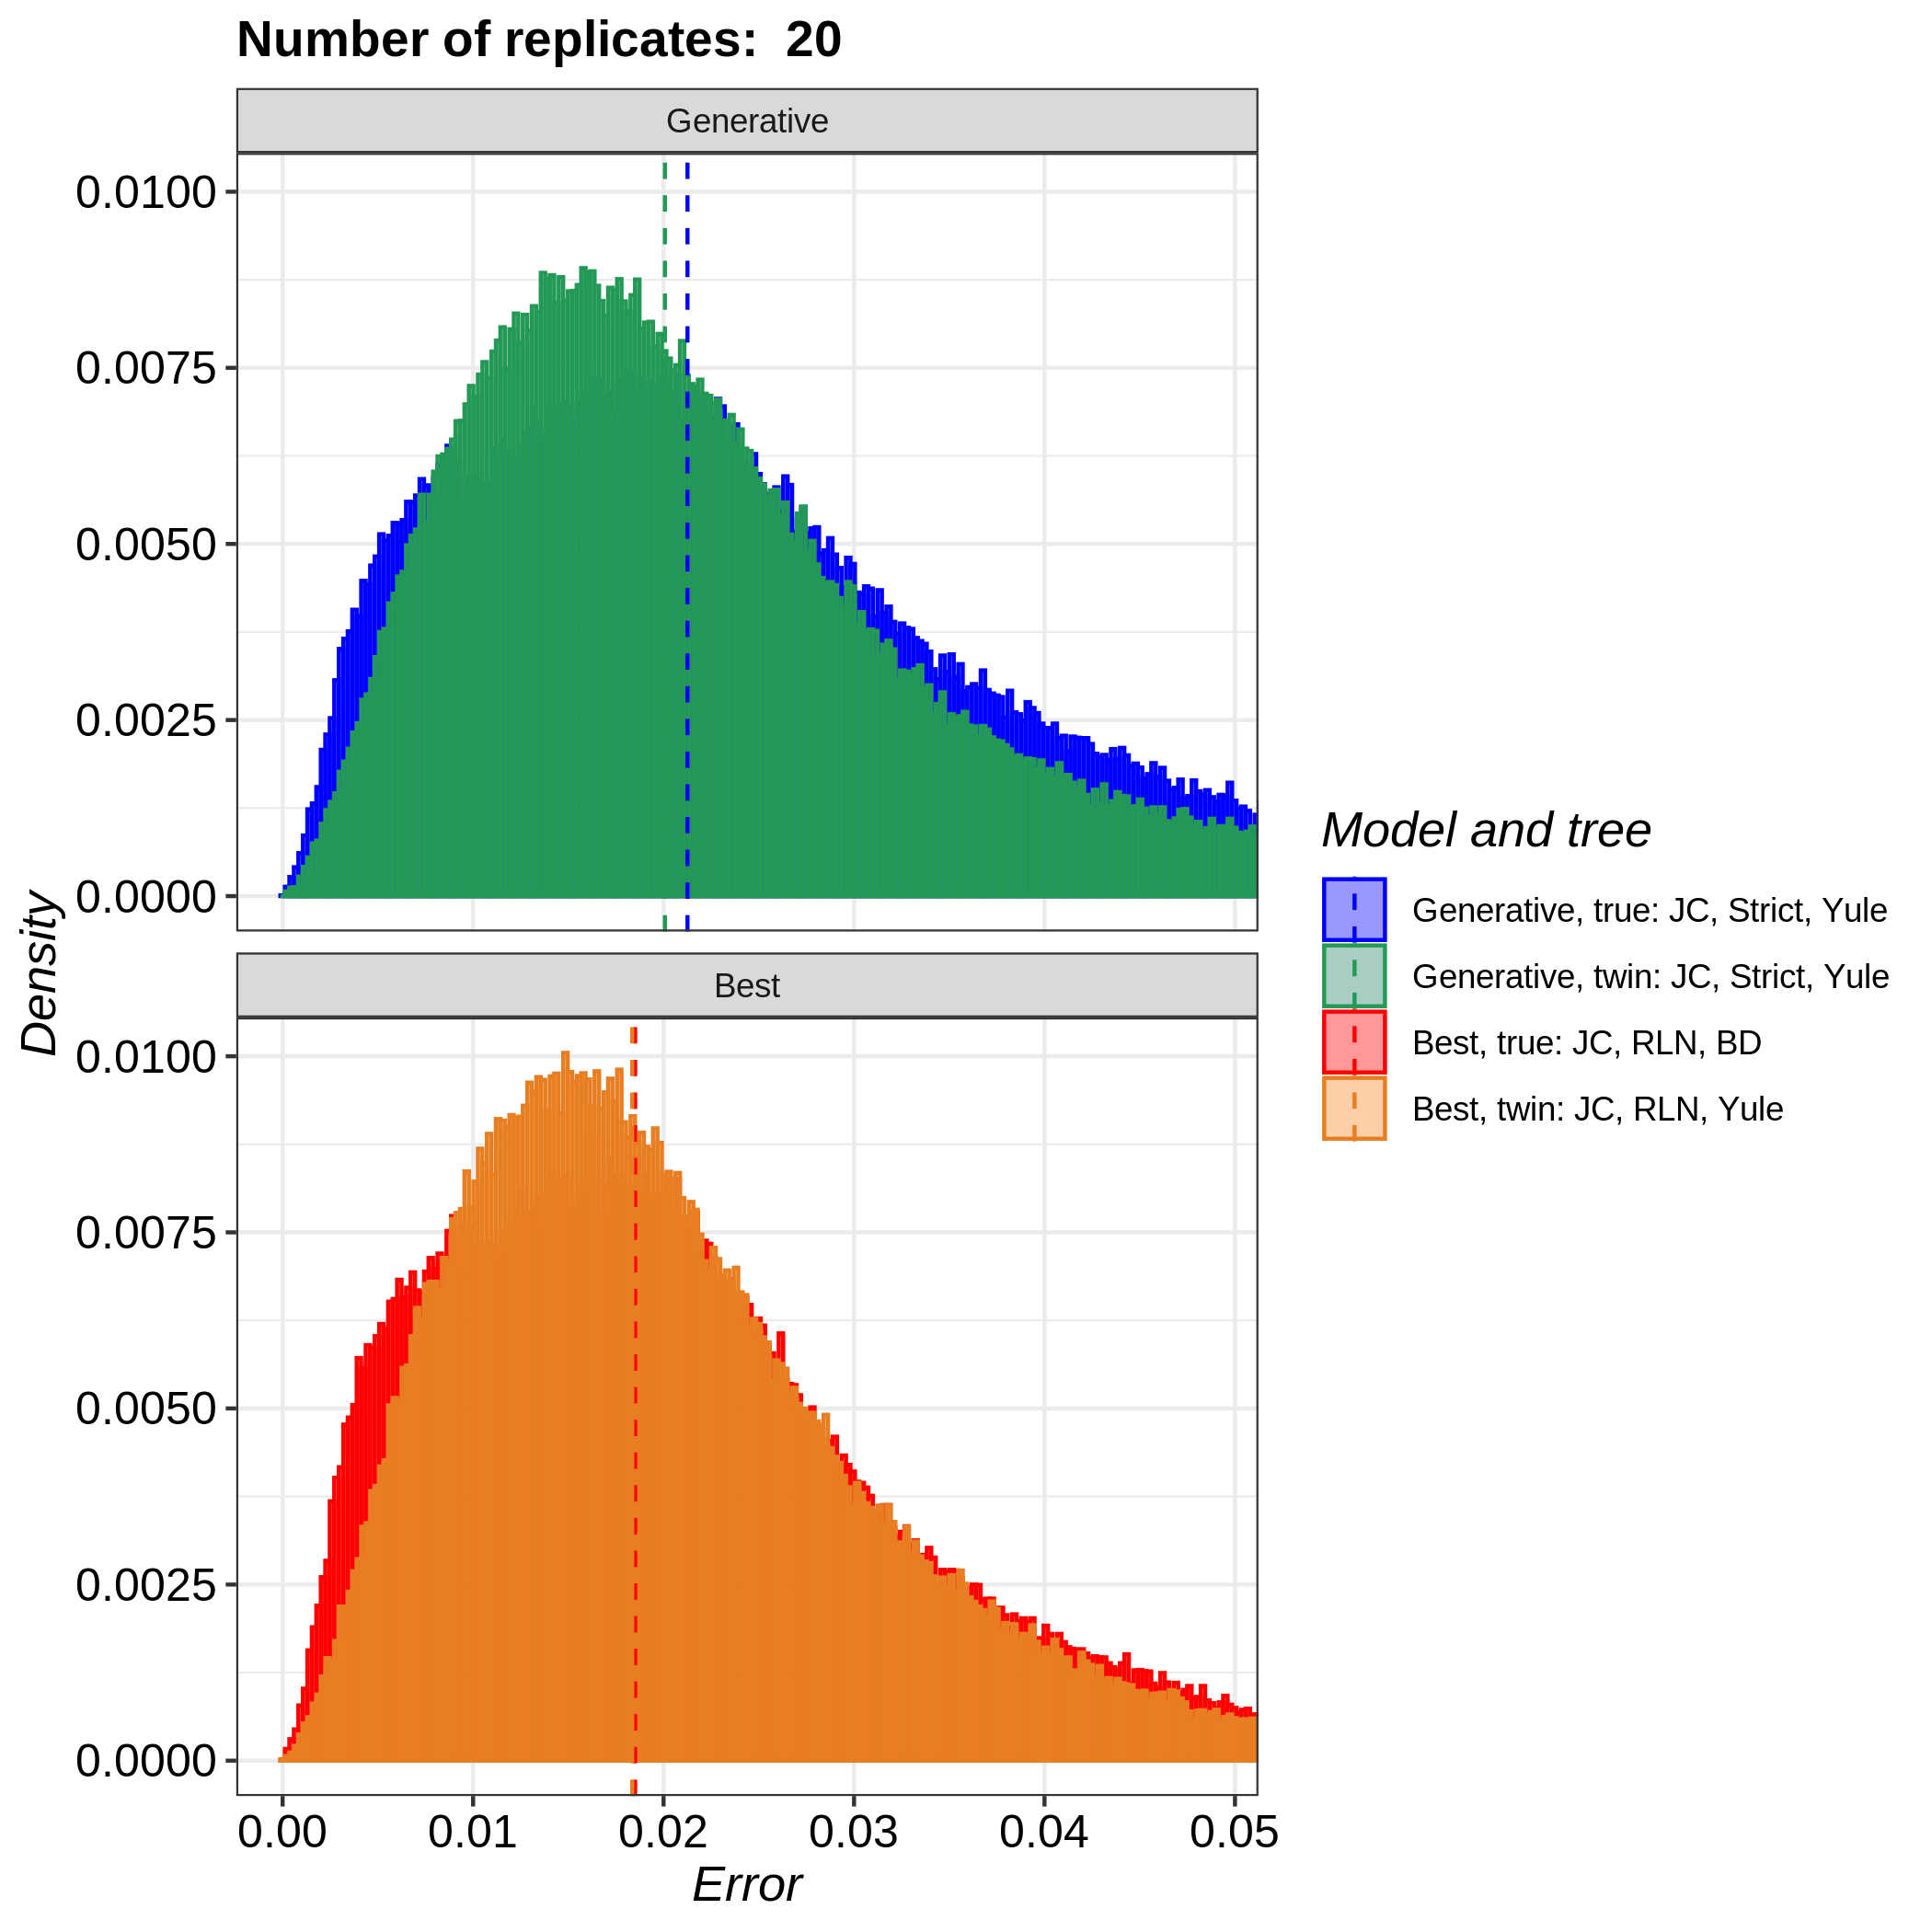
\includegraphics[width=0.98\textwidth]{pirouette_example_36/errors.png}
  \caption{Aggregate error distributions for 100 replicates,
    for the tree distribution presented 
    in \ref{subsec:distribution} but with a per-nucleotide mutation rate 
    of 0.50 / crown age. 
    This took 2.2 days (wall clock time) to compute.}
  \label{fig:example_0.50_mutation_rate}
\end{figure}

\begin{figure}[H]
  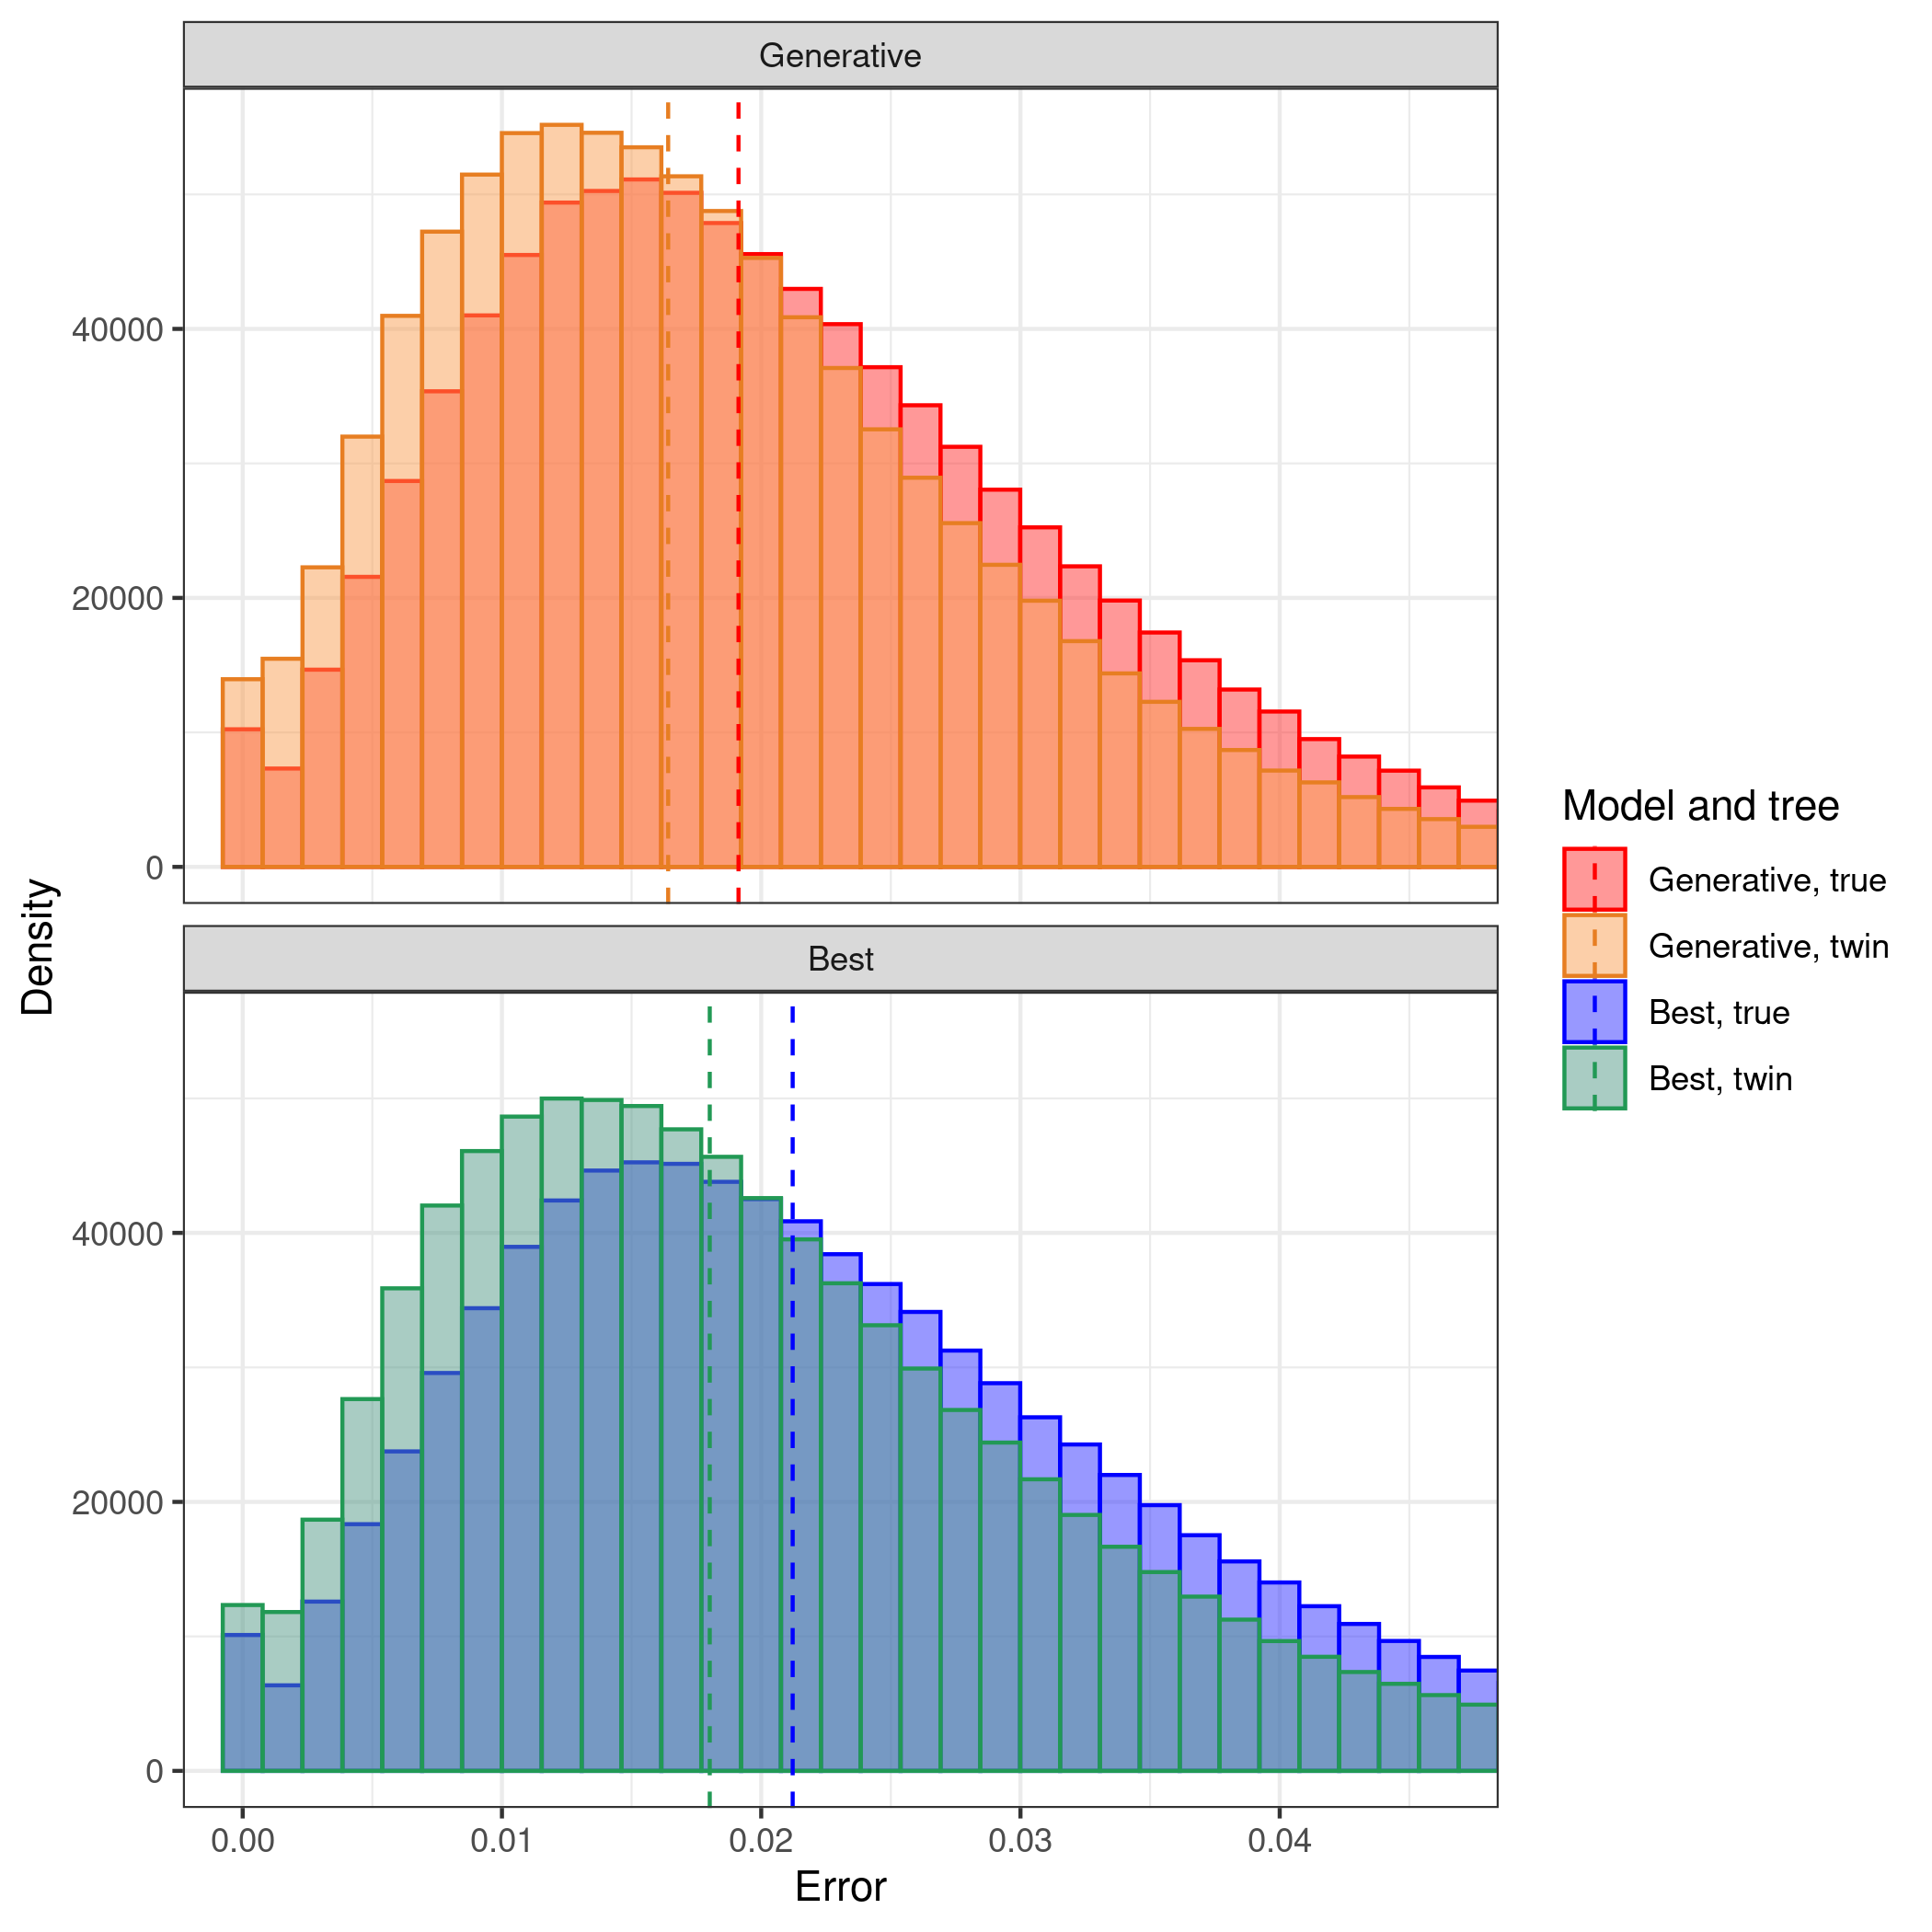
\includegraphics[width=0.98\textwidth]{pirouette_example_37/errors.png}
  \caption{Aggregate error distributions for 100 replicates,
    for the tree distribution presented 
    in \ref{subsec:distribution} but with a per-nucleotide mutation rate 
    of 0.75 / crown age. 
    This took 2.5 days (wall clock time) to compute.}
  \label{fig:example_0.75_mutation_rate}
\end{figure}

\begin{figure}[H]
  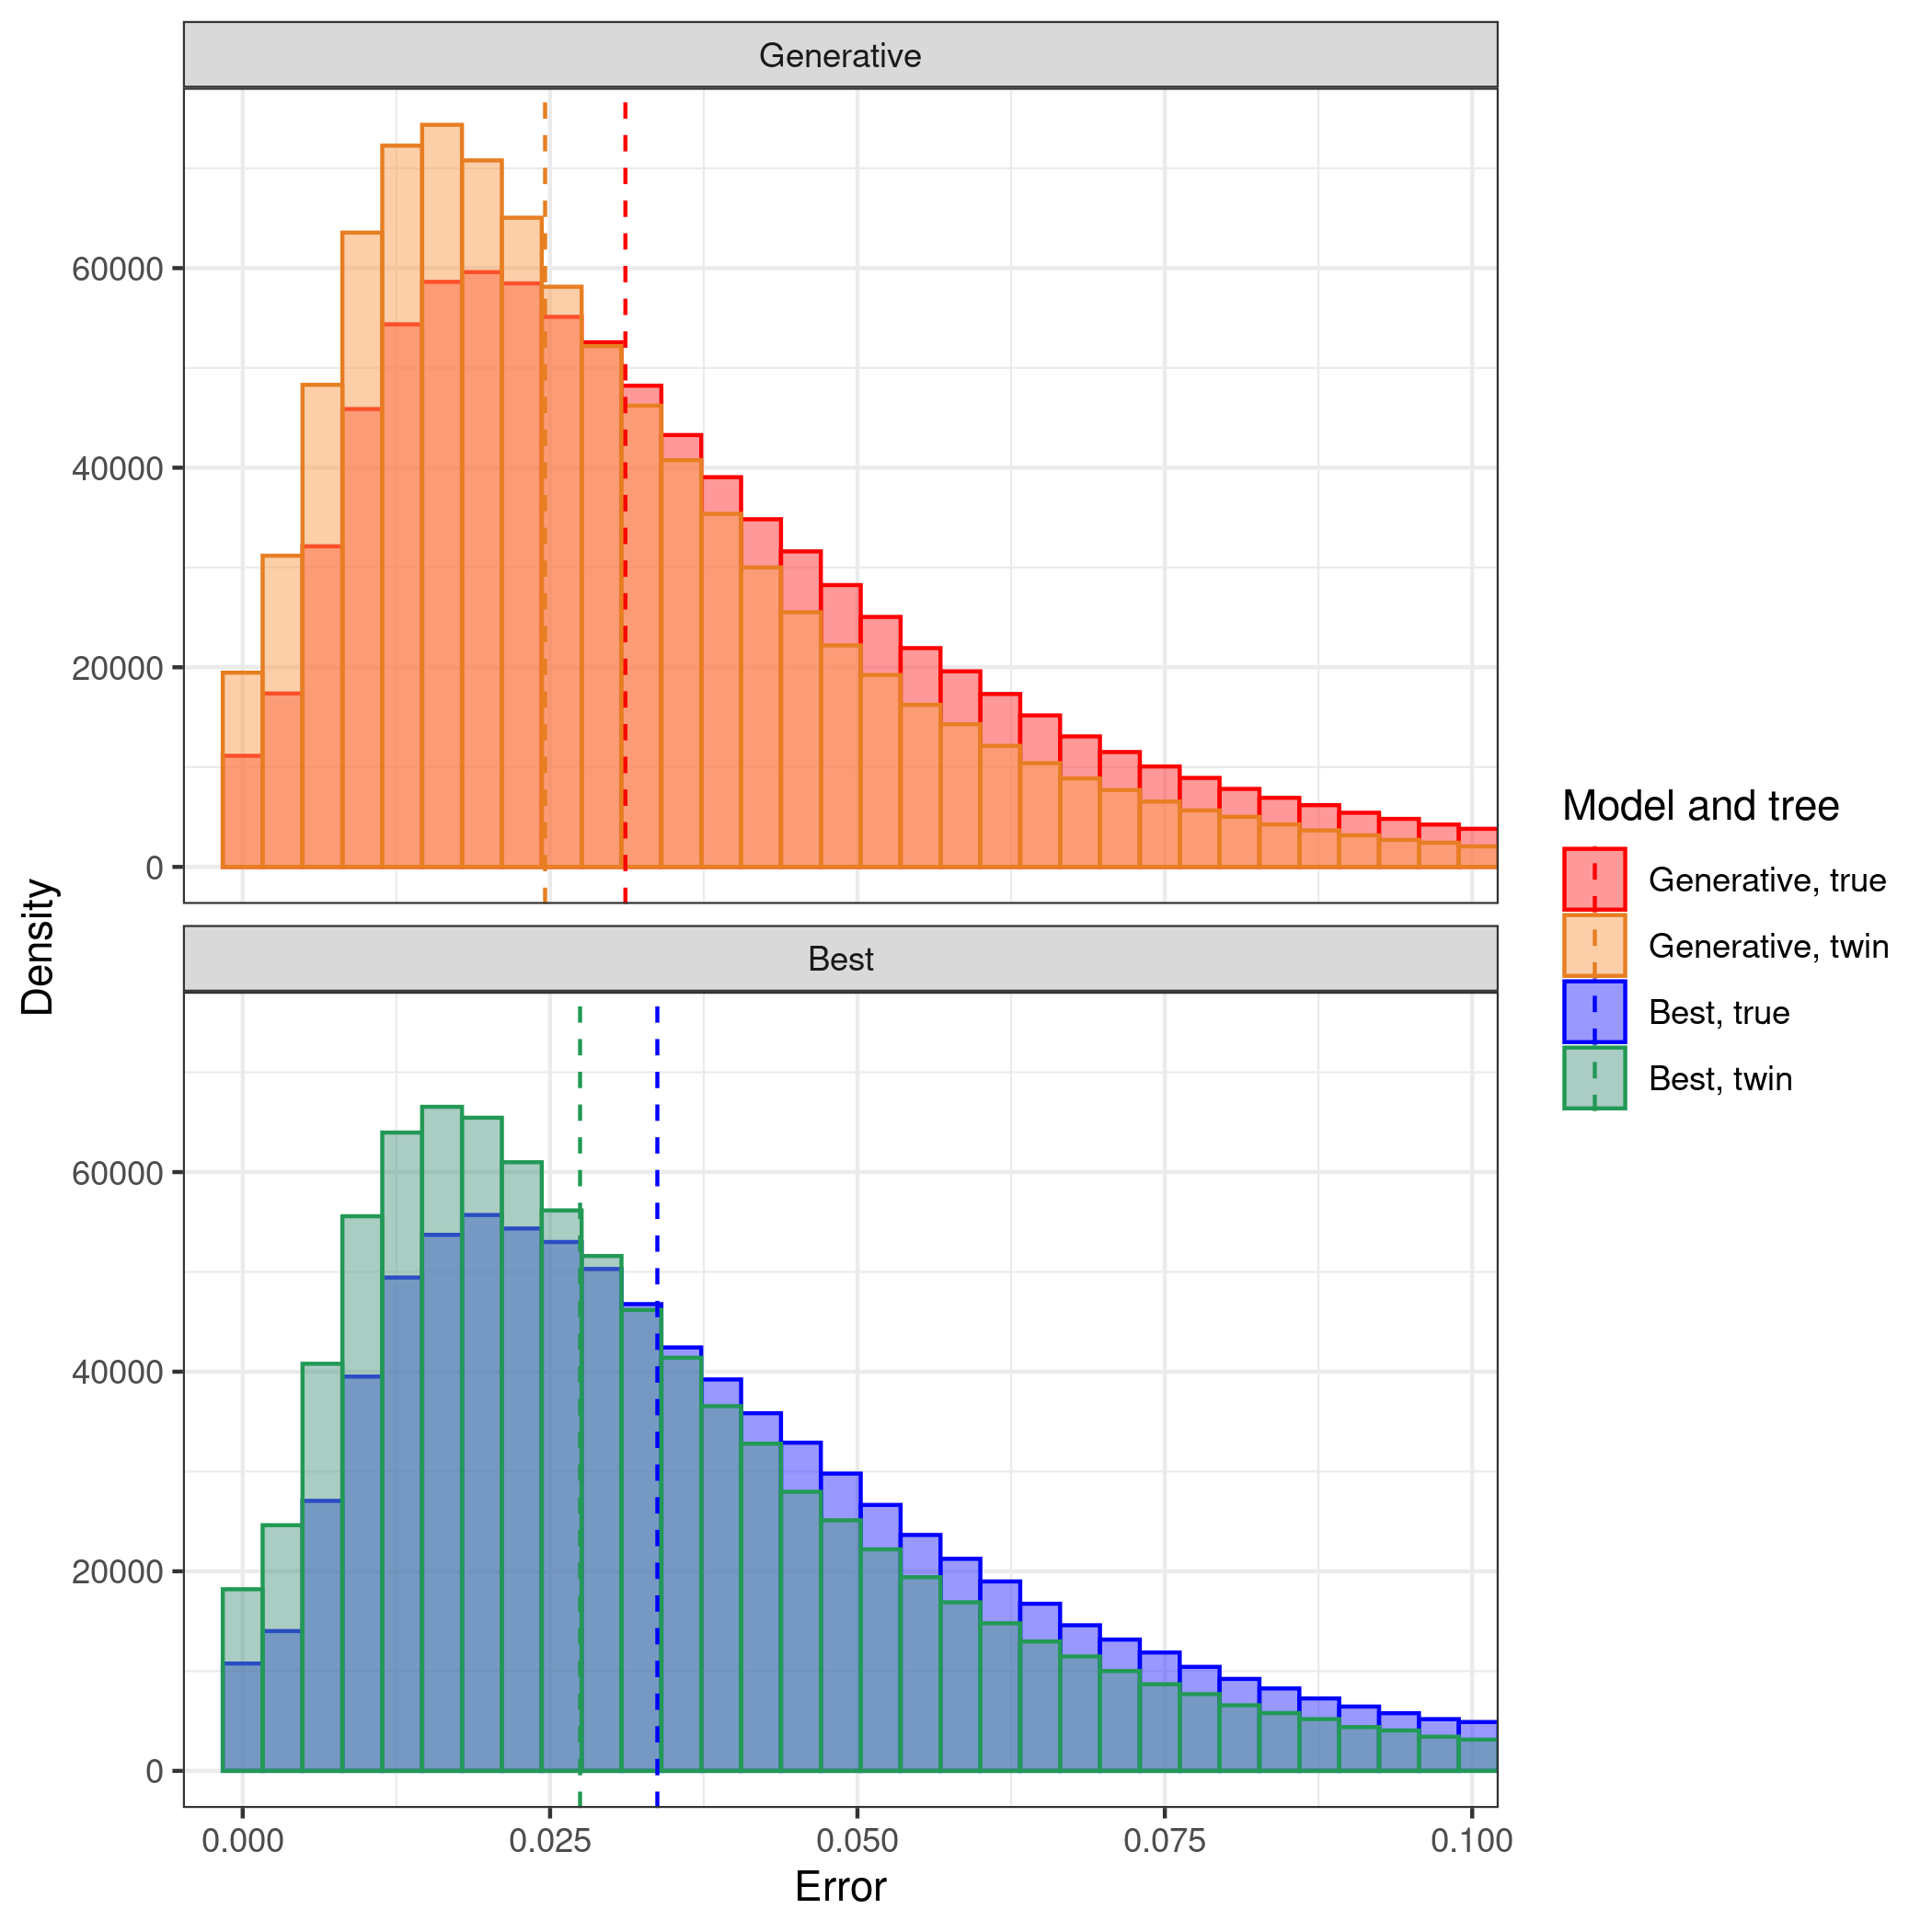
\includegraphics[width=0.98\textwidth]{pirouette_example_38/errors.png}
  \caption{Aggregate error distributions for 100 replicates,
    for the tree distribution presented 
    in \ref{subsec:distribution} but with a per-nucleotide mutation rate 
    of 1.25 / crown age. 
    This took 2.9 days (wall clock time) to compute.}
  \label{fig:example_1.25_mutation_rate}
\end{figure}

\begin{figure}[H]
  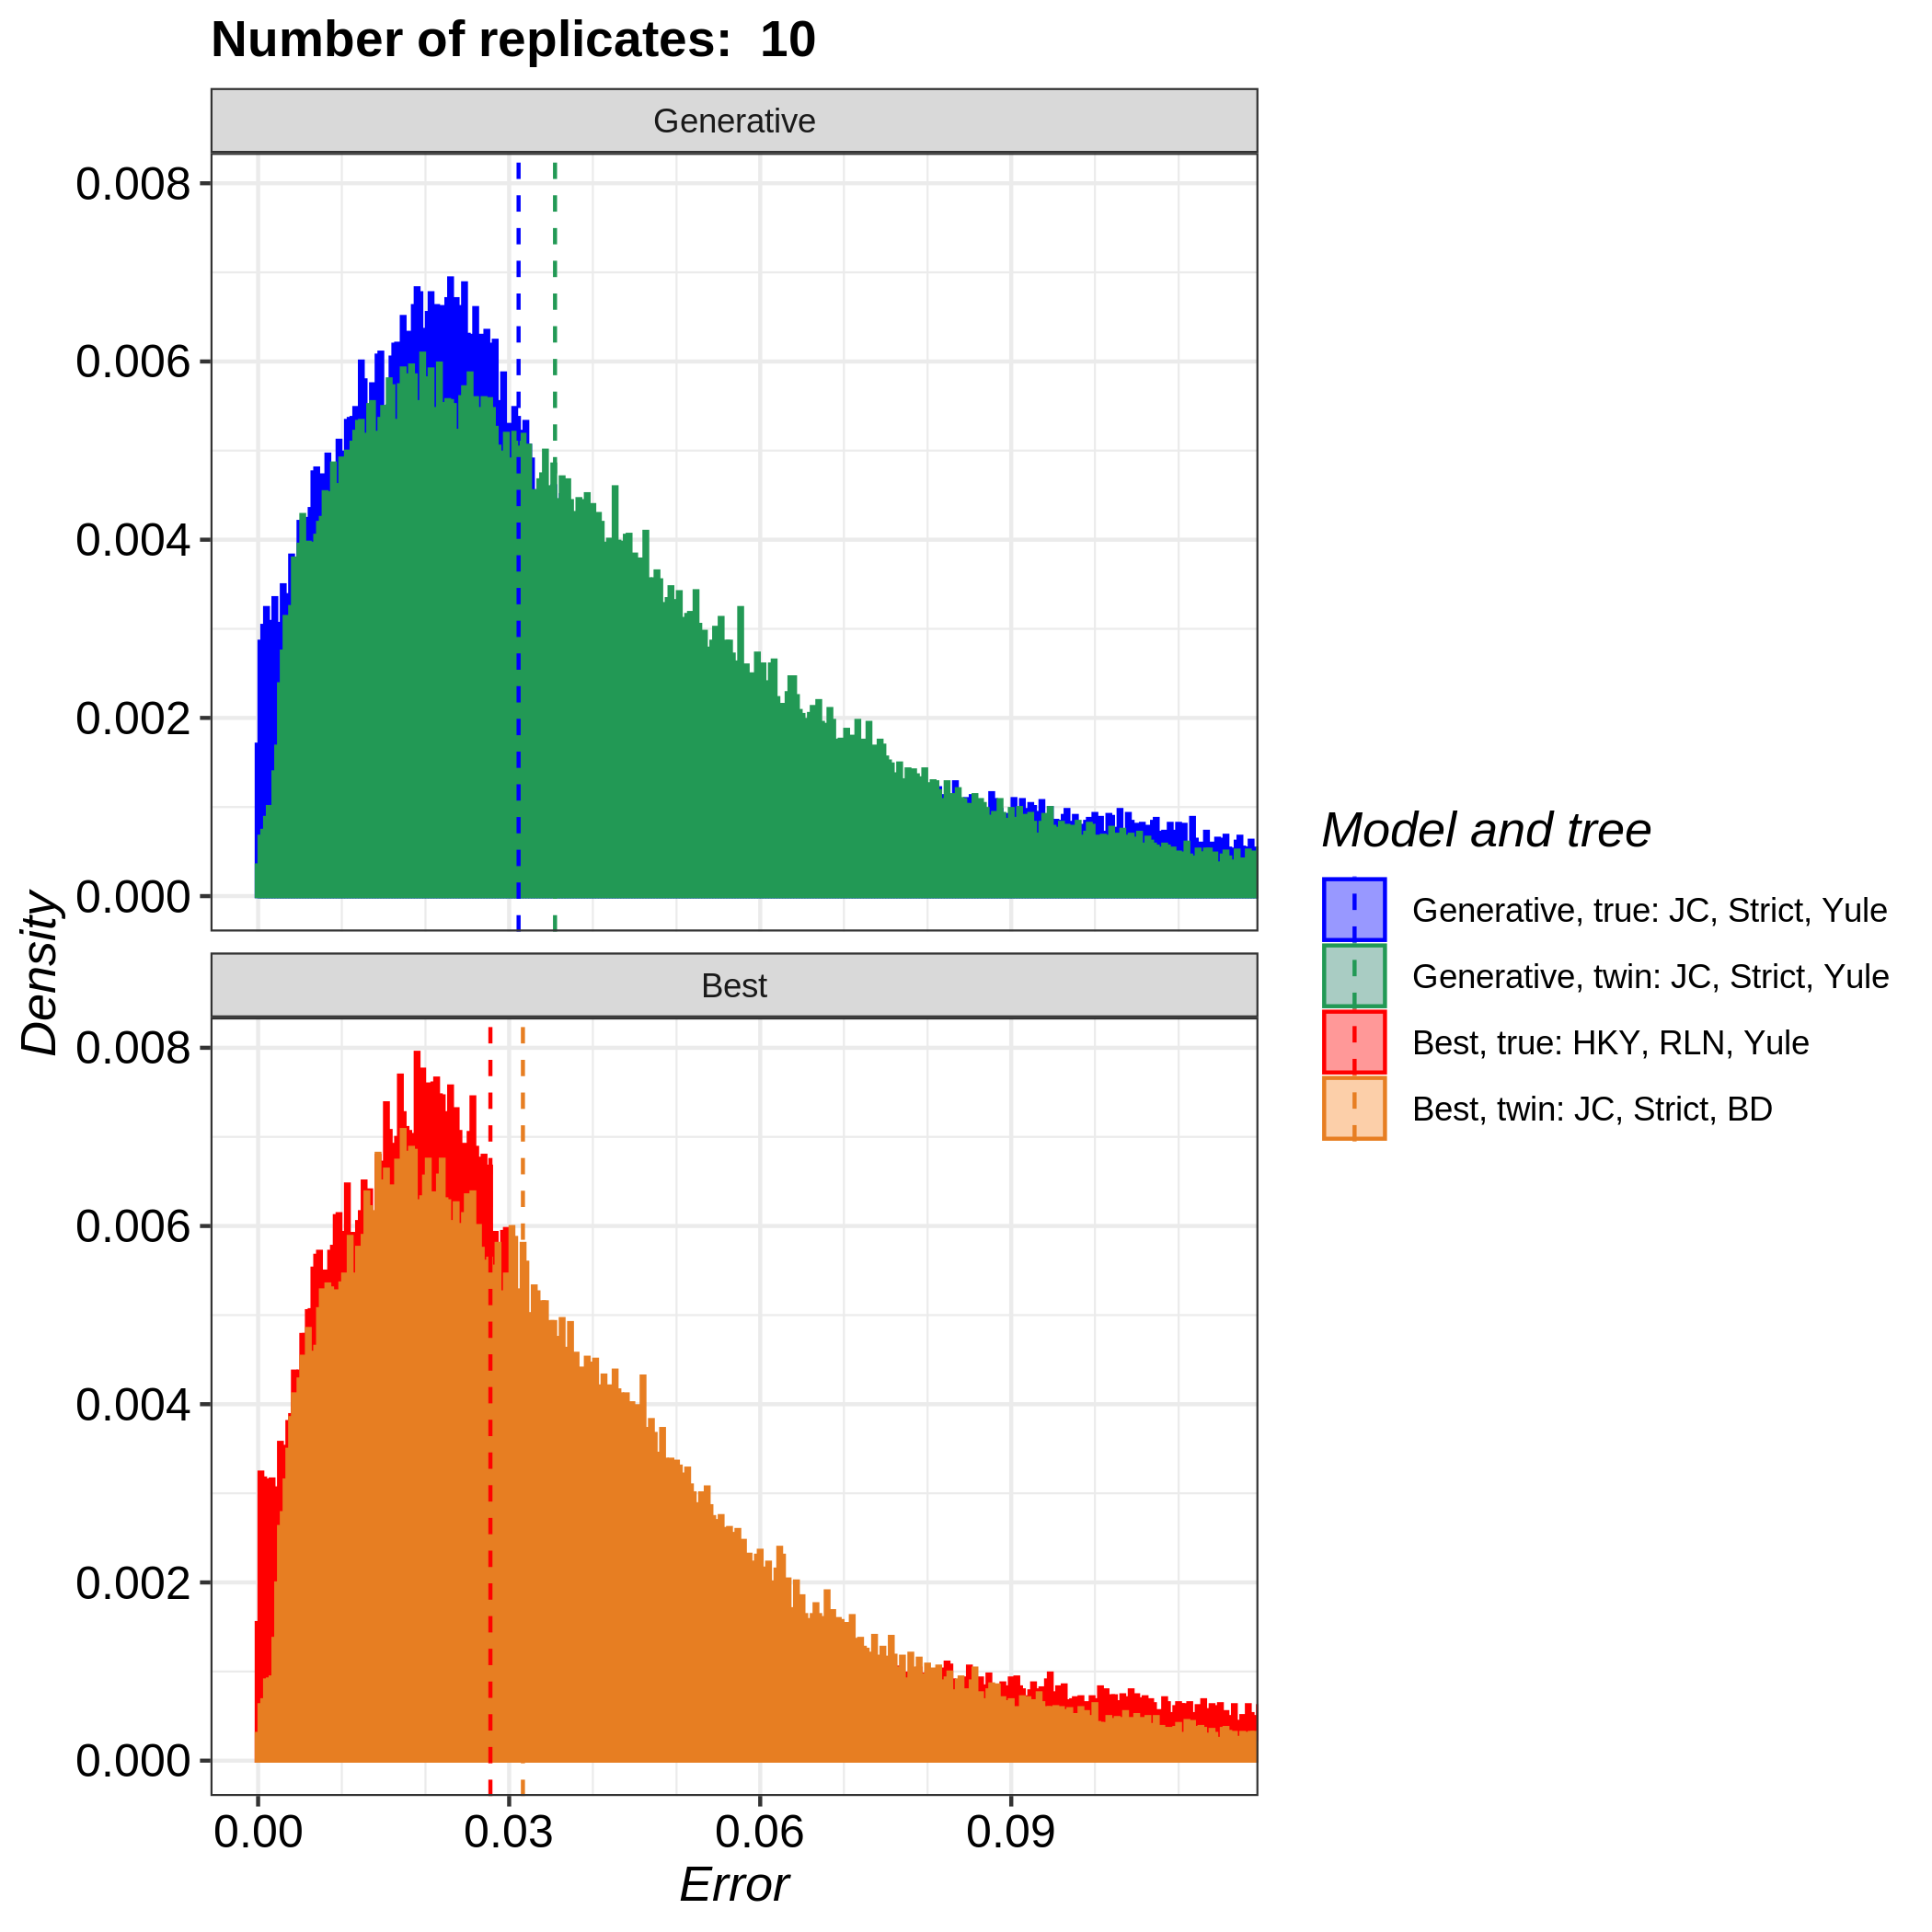
\includegraphics[width=0.98\textwidth]{pirouette_example_39/errors.png}
  \caption{Aggregate error distributions for 100 replicates,
    for the tree distribution presented 
    in \ref{subsec:distribution} but with a per-nucleotide mutation rate 
    of 1.50 / crown age. 
    This took 3.0 days (wall clock time) to compute.}
  \label{fig:example_1.50_mutation_rate}
\end{figure}

\begin{figure}[H]
  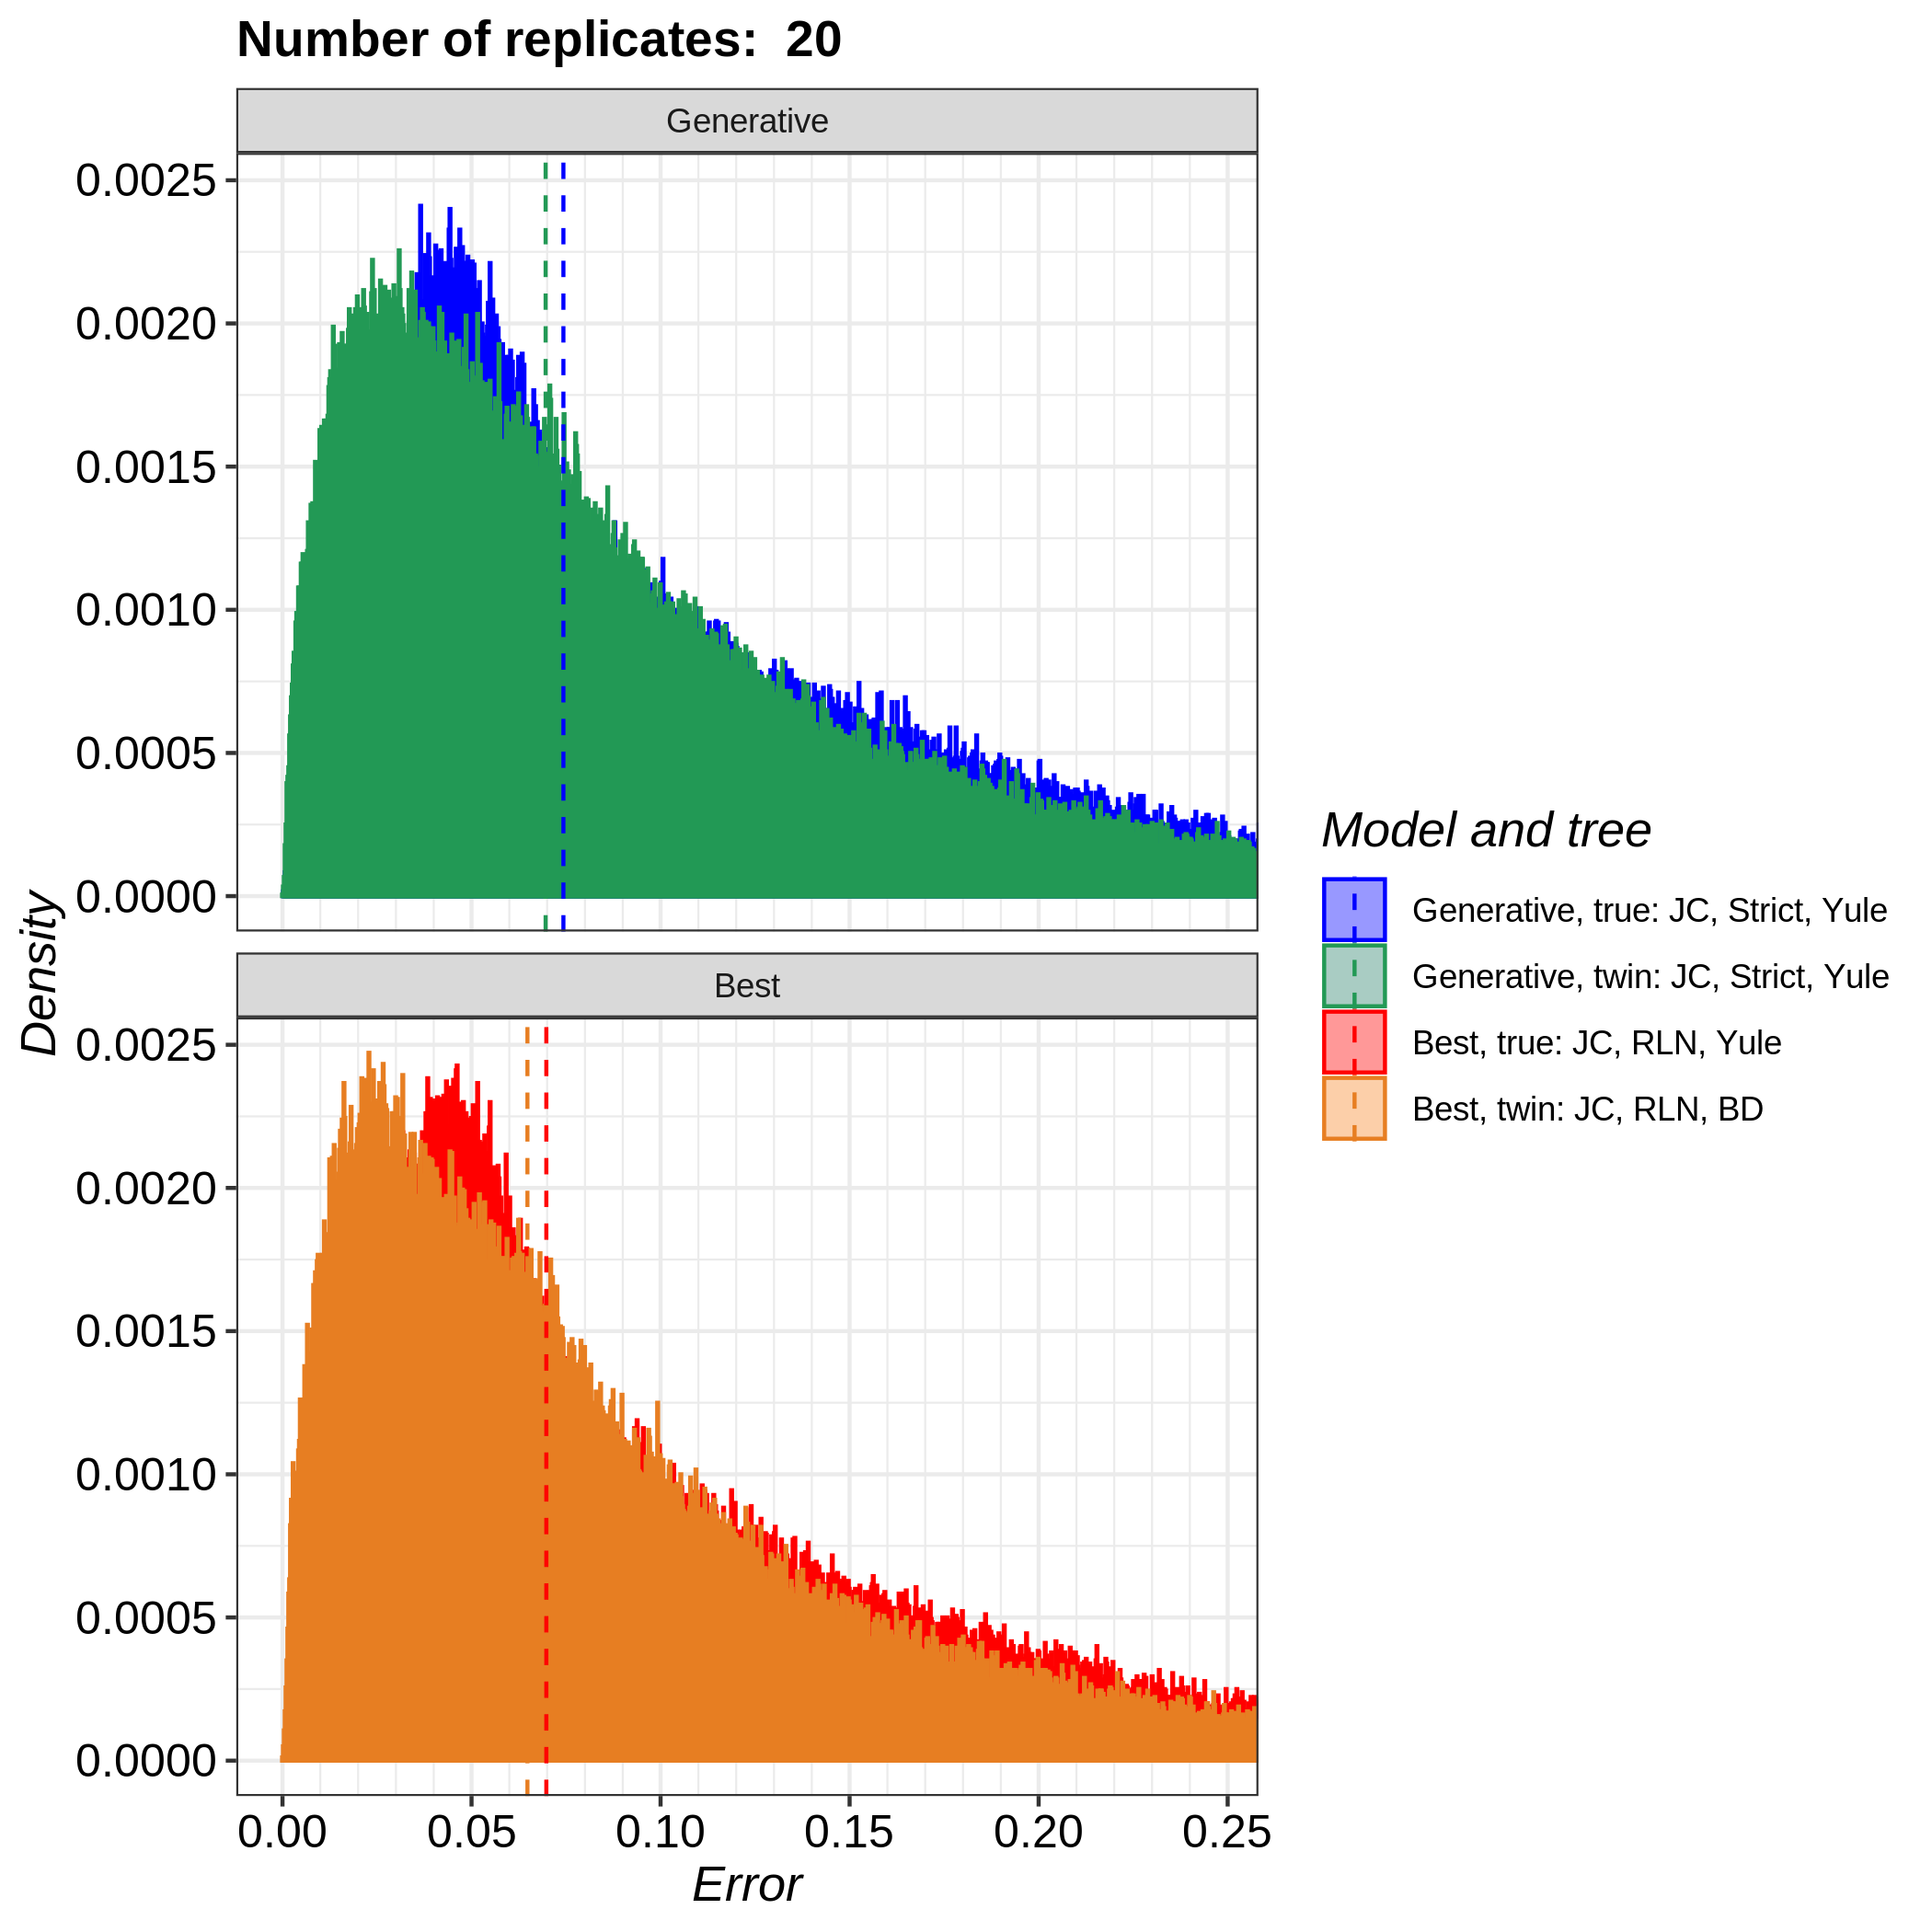
\includegraphics[width=0.98\textwidth]{pirouette_example_40/errors.png}
  \caption{Aggregate error distributions for 100 replicates,
    for the tree distribution presented 
    in \ref{subsec:distribution} but with a per-nucleotide mutation rate 
    of 2.0 / crown age. 
    This is done for 100 replicates.
    This took 3.0 days (wall clock time) to compute.}
  \label{fig:example_2.00_mutation_rate}
\end{figure}

\begin{figure}[H]
  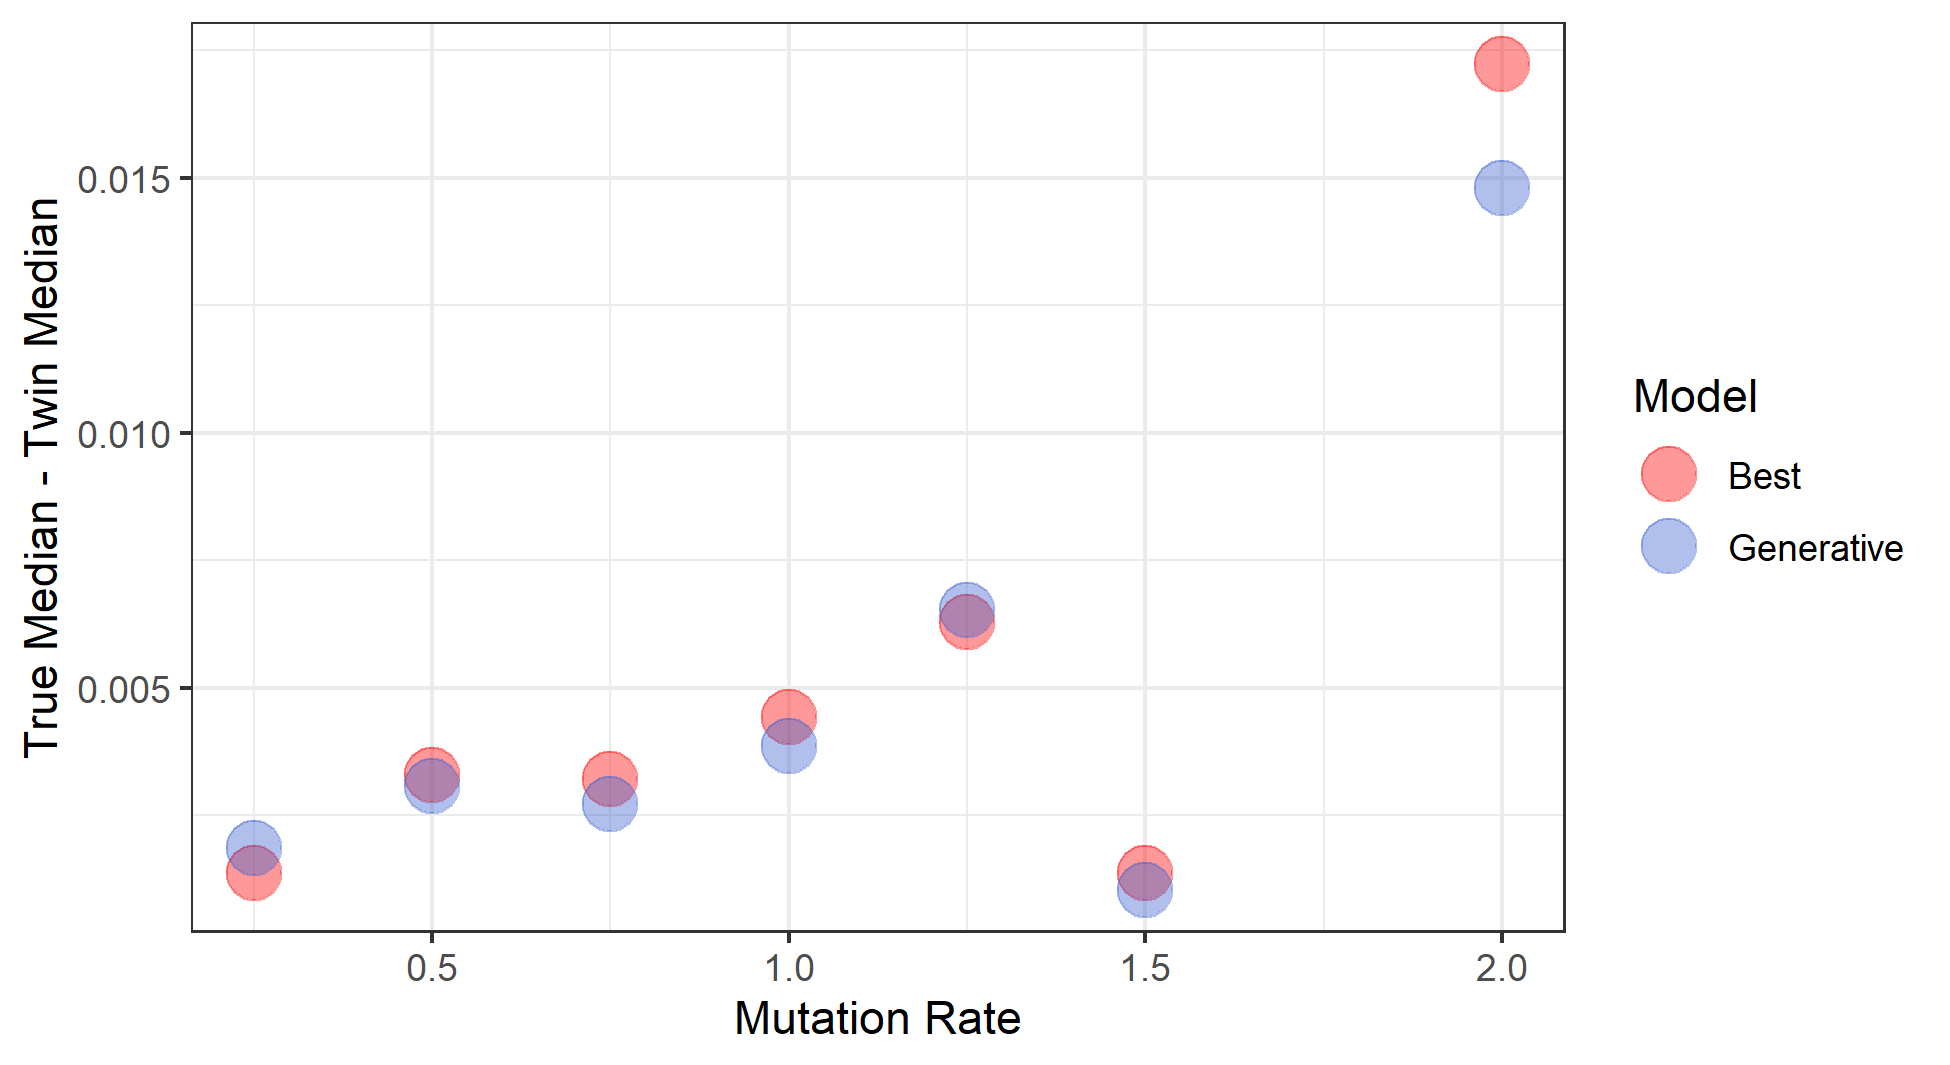
\includegraphics[width=0.98\textwidth]{supplementary_figures/plot_error_vs_mutation_rate.png}
  \caption{Difference between median true error and median twin error for different values of mutation rate.}
  \label{fig:error_vs_mutationrate}
\end{figure}

%%%%%%%%%%%%%%%%%%%%%%%%%%%%%%%%%%%%%%%%%%%%%%%%%%%%%%%%%%%%%%%%%%%%%%%%%%%%%%%%
\section{Acknowledgments}
\label{subsec:acknowledgments}
%%%%%%%%%%%%%%%%%%%%%%%%%%%%%%%%%%%%%%%%%%%%%%%%%%%%%%%%%%%%%%%%%%%%%%%%%%%%%%%%

We thank the Center for Information Technology of the University 
of Groningen for its support and for providing access to the Peregrine 
high performance computing cluster. 
We thank the Netherlands 
Organization for Scientific Research (NWO) for financial support 
through a VICI grant awarded to RSE.

%%%%%%%%%%%%%%%%%%%%%%%%%%%%%%%%%%%%%%%%%%%%%%%%%%%%%%%%%%%%%%%%%%%%%%%%%%%%%%%%
\section{Data accessibility}
\label{subsec:data_accessibility}
%%%%%%%%%%%%%%%%%%%%%%%%%%%%%%%%%%%%%%%%%%%%%%%%%%%%%%%%%%%%%%%%%%%%%%%%%%%%%%%%

All code is archived at 
\url{http://github.com/richelbilderbeek/pirouette_article},
with DOI \url{https://doi.org/12.3456/zenodo.1234567}.

%%%%%%%%%%%%%%%%%%%%%%%%%%%%%%%%%%%%%%%%%%%%%%%%%%%%%%%%%%%%%%%%%%%%%%%%%%%%%%%%
\section{Author contributions}
\label{subsec:author_contributions}
%%%%%%%%%%%%%%%%%%%%%%%%%%%%%%%%%%%%%%%%%%%%%%%%%%%%%%%%%%%%%%%%%%%%%%%%%%%%%%%%

RJCB, GL and RSE conceived the idea for the package. 
RJCB created, tested and revised the package.
GL provided major contributions to the package.
RJCB wrote the first draft of the manuscript, 
GL and RSE contributed to revisions.

%%%%%%%%%%%%%%%%%%%%%%%%%%%%%%%%%%%%%%%%%%%%%%%%%%%%%%%%%%%%%%%%%%%%%%%%%%%%%%%%
% Bibliography
%%%%%%%%%%%%%%%%%%%%%%%%%%%%%%%%%%%%%%%%%%%%%%%%%%%%%%%%%%%%%%%%%%%%%%%%%%%%%%%%
% MEE style
%\bibliographystyle{pirouette_mee}
% \bibliography{pirouette_supplement}
%\bibliography{pirouette_article}
%%%%%%%%%%%%%%%%%%%%%%%%%%%%%%%%%%%%%%%%%%%%%%%%%%%%%%%%%%%%%%%%%%%%%%%%%%%%%%%%



\end{document}
